%%% The main file. It contains definitions of basic parameters and includes all other parts.

%% Settings for single-side (simplex) printing
% Margins: left 40mm, right 25mm, top and bottom 25mm
% (but beware, LaTeX adds 1in implicitly)
\documentclass[12pt,a4paper]{report}
\setlength\textwidth{145mm}
\setlength\textheight{247mm}
\setlength\oddsidemargin{15mm}
\setlength\evensidemargin{15mm}
\setlength\topmargin{0mm}
\setlength\headsep{0mm}
\setlength\headheight{0mm}
% \openright makes the following text appear on a right-hand page
\let\openright=\clearpage

%% Settings for two-sided (duplex) printing
% \documentclass[12pt,a4paper,twoside,openright]{report}
% \setlength\textwidth{145mm}
% \setlength\textheight{247mm}
% \setlength\oddsidemargin{14.2mm}
% \setlength\evensidemargin{0mm}
% \setlength\topmargin{0mm}
% \setlength\headsep{0mm}
% \setlength\headheight{0mm}
% \let\openright=\cleardoublepage

%% Generate PDF/A-2u
\usepackage[a-2u]{pdfx}

%% Character encoding: usually latin2, cp1250 or utf8:
% \usepackage[utf8]{inputenc}

%% Prefer Latin Modern fonts
\usepackage{lmodern}

%% Further useful packages (included in most LaTeX distributions)
\usepackage{amsmath}        % extensions for typesetting of math
\usepackage{amsfonts}       % math fonts
\usepackage{amsthm}         % theorems, definitions, etc.
\usepackage{bbding}         % various symbols (squares, asterisks, scissors, ...)
\usepackage{bm}             % boldface symbols (\bm)
\usepackage{graphicx}       % embedding of pictures
\usepackage{fancyvrb}       % improved verbatim environment
\usepackage{natbib}         % citation style AUTHOR (YEAR), or AUTHOR [NUMBER]
\usepackage[nottoc]{tocbibind} % makes sure that bibliography and the lists
			    % of figures/tables are included in the table
			    % of contents
\usepackage{dcolumn}        % improved alignment of table columns
\usepackage{booktabs}       % improved horizontal lines in tables
\usepackage{paralist}       % improved enumerate and itemize
\usepackage[usenames]{xcolor}  % typesetting in color
\usepackage{float}
\usepackage{subcaption}
\usepackage{caption}
\usepackage{wrapfig}
\usepackage{fontspec}
\usepackage{multirow}
\usepackage{longtable}
\usepackage{xunicode} %% loading this first to avoid clash with bidi/arabic
\usepackage{polyglossia}
\usepackage{algorithmic}
% \usepackage{algcompatible}
\usepackage{algorithm}
\usepackage{siunitx}
\usepackage{multicol}
\usepackage{soul}
\setlength{\columnsep}{5mm}
\usepackage{tikz}
\usepackage{mathtools}
\usetikzlibrary{shapes,arrows,fit,calc}

\tikzstyle{decision} = [diamond, draw=black, thick, fill=blue!20, 
    text width=5em, text centered, node distance=3cm, inner sep=0pt]
\tikzstyle{block} = [rectangle, draw=black, thick, fill=blue!20, 
    text width=5em, text centered, rounded corners, minimum height=4em]
\tikzstyle{line} = [draw, thick, -latex']


\renewcommand{\algorithmicrequire}{\textbf{Input:}}
\renewcommand{\algorithmicensure}{\textbf{Output:}}

\setdefaultlanguage[]{english}
\setotherlanguages{russian,hindi,hebrew,arabic}
\newfontfamily\devanagarifont[Script=Devanagari]{BABEL Unicode}
\newfontfamily\cyrillicfont[Script=Cyrillic]{Charis SIL}
\newfontfamily\hebrewfont[Script=Hebrew]{Noto Sans Hebrew}
\newfontfamily\arabicfont[Script=Arabic]{Noto Naskh Arabic}
% \setkeys{hindi}{numerals=Western}
%%% Basic information on the thesis

% Thesis title in English (exactly as in the formal assignment)
\def\ThesisTitle{Consistency of Linguistic Annotation}

% Author of the thesis
\def\ThesisAuthor{Akshay Aggarwal}

% Year when the thesis is submitted
\def\YearSubmitted{2020}

% Name of the department or institute, where the work was officially assigned
% (according to the Organizational Structure of MFF UK in English,
% or a full name of a department outside MFF)
\def\Department{Institute of Formal and Applied Linguistics}

% Is it a department (katedra), or an institute (ústav)?
\def\DeptType{Institute}

% Thesis supervisor: name, surname and titles
\def\Supervisor{RNDr. Daniel Zeman, PhD}
\def\CoSupervisor{Koldo Gojenola, PhD}

% Supervisor's department (again according to Organizational structure of MFF)
\def\SupervisorsDepartment{Institute of Formal and Applied Linguistics}
\def\CoSupervisorsDepartment{Computer Languages and Systems, University of Basque Country (UPV-EHU), Spain}

% Study programme and specialization
\def\StudyProgramme{Computer Science}
\def\StudyBranch{Computational Linguistics}

% An optional dedication: you can thank whomever you wish (your supervisor,
% consultant, a person who lent the software, etc.)
\def\Dedication{%

I would like to express my gratitude to my supervisors, Daniel Zeman from Charles University for his dedicated guidance as well as his recommendation of the thesis topic; and Koldo Gojenola from UPV/EHU for his valuable remarks and the much needed push to allow me to keep things structured.

I am very thankful to Prof. Mark\'eta Lopatkov\'a and Prof. Vladislav Kubo\v n from Charles University, Prague and also Dr. Bobbye Pernice from Universit\"at des Saarlandes for their immense help in handling all the difficulties encountered during the two years of studying in LCT programme.

A very special note of thanks is extended to Chiara Alzetta of ItaliaNLP Lab for her constant help in an experiment. From the discussion about the algorithm, to actually running it, the experiment on lisca tools would not have been possible without her valuable inputs.

A very sincere vote of thanks is also extended to Charles University in Prague for the university's provision of computing and storage resources. A very heartfelt thanks is also due, to the brilliant researchers and teachers therein. The thesis would not have been possible without their brilliant shaping of the foundations of the subject within me.

Computational resources were supplied by the Ministry of Education, Youth and Sports of the Czech Republic under the Projects CESNET (Project No. LM2015042) and CERIT-Scientific Cloud (Project No. LM2015085) provided within the program Projects of Large Research, Development and Innovations Infrastructures.

Finally, I would like to thank all the people who supported me during the two and a half years, my family and friends. Special thanks are due to my friends in Prague for helping me keep my sanity in place.}

% Abstract (recommended length around 80-200 words; this is not a copy of your thesis assignment!)
\def\Abstract{%
This research attempts at identification and correction of inconsistencies in different treebanks. The inconsistencies might be related to linguistic constructions, failure of the guidelines of annotation, failure to understand the guidelines on annotator's part, or random errors caused by annotators, among others. The work also proposes a metric to test the similarity of different treebanks in the same language, when the annotation guidelines remain the same. We offer solutions to some previously identified inconsistencies in the scope of the Universal Dependencies Project in a language neutral manner, the solutions being reliable enough to not need a human annotator in the pipeline.
}

% 3 to 5 keywords (recommended), each enclosed in curly braces
\def\Keywords{%
{Annotation Consistency} {Annotation Inconsistency} {Error Mining} {Language Independent} {Universal Dependencies} {UD Project} {Syntax} {Morphology}
}

%% The hyperref package for clickable links in PDF and also for storing
%% metadata to PDF (including the table of contents).
%% Most settings are pre-set by the pdfx package.
\hypersetup{unicode}
\hypersetup{breaklinks=true}

% Definitions of macros (see description inside)
%%% This file contains definitions of various useful macros and environments %%%
%%% Please add more macros here instead of cluttering other files with them. %%%

%%% Minor tweaks of style

% These macros employ a little dirty trick to convince LaTeX to typeset
% chapter headings sanely, without lots of empty space above them.
% Feel free to ignore.
\makeatletter
\def\@makechapterhead#1{
  {\parindent \z@ \raggedright \normalfont
   \Huge\bfseries \thechapter. #1
   \par\nobreak
   \vskip 20\p@
}}
\def\@makeschapterhead#1{
  {\parindent \z@ \raggedright \normalfont
   \Huge\bfseries #1
   \par\nobreak
   \vskip 20\p@
}}
\makeatother

% This macro defines a chapter, which is not numbered, but is included
% in the table of contents.
\def\chapwithtoc#1{
\chapter*{#1}
\addcontentsline{toc}{chapter}{#1}
}

% Draw black "slugs" whenever a line overflows, so that we can spot it easily.
\overfullrule=1mm

%%% Macros for definitions, theorems, claims, examples, ... (requires amsthm package)

\theoremstyle{plain}
\newtheorem{thm}{Theorem}
\newtheorem{lemma}[thm]{Lemma}
\newtheorem{claim}[thm]{Claim}

\theoremstyle{remark}
\newtheorem*{cor}{Corollary}
\newtheorem*{rem}{Remark}
\newtheorem{example}{Example}

\theoremstyle{definition}
\newtheorem{definition}{Definition}

%%% An environment for typesetting of program code and input/output
%%% of programs. (Requires the fancyvrb package -- fancy verbatim.)

\DefineVerbatimEnvironment{code}{Verbatim}{fontsize=\small, frame=single}

%%% The field of all real and natural numbers
\newcommand{\R}{\mathbb{R}}
\newcommand{\N}{\mathbb{N}}

%%% Useful operators for statistics and probability
\DeclareMathOperator{\pr}{\textsf{P}}
\DeclareMathOperator{\E}{\textsf{E}\,}
\DeclareMathOperator{\var}{\textrm{var}}
\DeclareMathOperator{\sd}{\textrm{sd}}

%%% Various math goodies
\newcommand{\goto}{\rightarrow}
\newcommand{\gotop}{\stackrel{P}{\longrightarrow}}
\newcommand{\maon}[1]{o(n^{#1})}
\newcommand{\abs}[1]{\left|{#1}\right|}
\newcommand{\dint}{\int_0^\tau\!\!\int_0^\tau}
\newcommand{\isqr}[1]{\frac{1}{\sqrt{#1}}}

%%% Various table goodies
\newcommand{\pulrad}[1]{\raisebox{1.5ex}[0pt]{#1}}
\newcommand{\mc}[1]{\multicolumn{1}{c}{#1}}

\newenvironment{reusefigure}[2][htbp]
  {\addtocounter{figure}{-1}%
   \renewcommand{\theHfigure}{dupe-fig}% If you're using hyperref
   \renewcommand{\thefigure}{\ref{#2}}% Figure counter is \ref
   \renewcommand{\addcontentsline}[3]{}% Avoid placing figure in LoF
   \begin{figure}[#1]}
  {\end{figure}}

% Title page and various mandatory informational pages
\begin{document}

%%% Title page of the thesis and other mandatory pages

%%% Title page of the thesis

\pagestyle{empty}
\hypersetup{pageanchor=false}
\begin{center}

\centerline{\mbox{
\includegraphics[width=166mm]{img/logo-en.pdf}}}

\vspace{-8mm}
\vfill

{\bf\Large MASTER THESIS}

\vfill

{\LARGE\ThesisAuthor}

\vspace{15mm}

{\LARGE\bfseries\ThesisTitle}

\vfill

\Department

\vfill

\begin{tabular}{rl}

Supervisor of the master thesis: & \Supervisor \\
& \CoSupervisor \\
\noalign{\vspace{2mm}}
Study programme: & \StudyProgramme \\
\noalign{\vspace{2mm}}
Study branch: & \StudyBranch \\
\end{tabular}

\vfill

% Zde doplňte rok
Prague \YearSubmitted

\end{center}

\newpage

%%% Here should be a bound sheet included -- a signed copy of the "master
%%% thesis assignment". This assignment is NOT a part of the electronic
%%% version of the thesis. DO NOT SCAN.

%%% A page with a solemn declaration to the master thesis

\openright
\hypersetup{pageanchor=true}
\pagestyle{plain}
\pagenumbering{roman}
\vglue 0pt plus 1fill

\noindent
I declare that I carried out this master thesis independently, and only with the cited
sources, literature and other professional sources.

\medskip\noindent
I understand that my work relates to the rights and obligations under the Act No.~121/2000 Sb.,
the Copyright Act, as amended, in particular the fact that the Charles
University has the right to conclude a license agreement on the use of this
work as a school work pursuant to Section 60 subsection 1 of the Copyright Act.

\vspace{10mm}

\hbox{\hbox to 0.5\hsize{%
In ........ date ............	% FIXME!
\hss}\hbox to 0.5\hsize{%
signature of the author
\hss}}

\vspace{20mm}
\newpage

%%% Dedication

\openright

\noindent
\Dedication

\newpage

%%% Mandatory information page of the thesis

\openright

\vbox to 0.5\vsize{
\setlength\parindent{0mm}
\setlength\parskip{5mm}

Title:
\ThesisTitle

Author:
\ThesisAuthor

\DeptType:
\Department

Supervisors:
\Supervisor, \SupervisorsDepartment; \CoSupervisor, \CoSupervisorsDepartment

Abstract:
\Abstract

Keywords:
\Keywords

\vss}

\newpage

\openright
\pagestyle{plain}
\pagenumbering{arabic}
\setcounter{page}{1}


%%% A page with automatically generated table of contents of the master thesis

\tableofcontents

%%% Abbreviations used in the thesis, if any, including their explanation
%%% In mathematical theses, it could be better to move the list of abbreviations to the beginning of the thesis.
\chapwithtoc{List of Abbreviations}
\begin{itemize}
    \item \textbf{CLAS}- Content-based Labelled Attachment Score
    \item \textbf{GS}- Gold Standard
    \item \textbf{LTR}- Left To Right written order language
    \item \textbf{MWE}- Multi-Word Entity
    \item \textbf{NER}- Named Entity Recognition
    \item \textbf{PCA}- Principal Component Analysis
    \item \textbf{POS}- Part Of Speech
    \item \textbf{RTL}- Right To Left written order language
    \item \textbf{sd}- Standard Deviation
    \item \textbf{SOTA}- State Of The Art
    \item \textbf{TAME}- Time, Aspect, Modality, Evidentiality
    \item \textbf{UD}- Universal Dependencies
\end{itemize}

%%% Each chapter is kept in a separate file
% the pages count refers to experiments completed, in the document


    \chapter{Introduction}

According to Wikipedia definition of the word\footnote{\url{https://en.wikipedia.org/wiki/Treebank}}, a treebank is a parsed text corpus, which annotates syntactic or semantic structure. Built usually (but not always) on top of a POS-annotated corpus, a treebank might seek to include phrase structure (Example- PennTreebank \citep{PennTreebank}), dependency structure (Example- Prague Dependency Treebank \citep{PDT}) or semantic information (Example- FrameNet \citep{framenet}).

A treebank can be constructed manually, by linguists spending a considerable time developing the treebank; or semi-automatically, wherein the data is automatically annotated, and then checked for consistency. Regardless of the method used for its creation, a treebank is an essential element in the field of computational linguistics. A treebank can be used to study linguistic structures, find out features associated with a language, or to understand the constructional peculiarities within a language, among others. 

In this work, our main focus is on syntactic treebanks and especially dependency treebanks, rather than semantic ones. Therefore, the term `treebank' shall be used to refer to a syntactic (dependency) treebank henceforth, unless specified otherwise.

\section{Inter-conversion of Treebanks}

There exist a multitude of treebanks for different languages as they can be seen on Wikipedia\footnote{\url{https://en.wikipedia.org/wiki/Treebank\#Syntactic_treebanks}}, for example. As noted by \cite{kakkonen2006}, there exist a variety of formats and annotation schemes even for the treebanks for the same language. A well known example to this is the case of distinctive POS tagging schemes for PennTreebank\footnote{\url{https://www.ling.upenn.edu/courses/Fall_2003/ling001/penn_treebank_pos.html}} and for British National Corpus\footnote{\url{http://www.natcorp.ox.ac.uk/docs/c5spec.html}}, both of which are meant for annotation of English language. \citeauthor{kakkonen2006}, in his work also notices that there exist tools which are meant to work for a particular tagset/annotation scheme. Given enough similarities in annotation schemes, a (automatic) conversion process can be drafted from one annotation schema to another.

This conversion process of a treebank from one annotation scheme to another can be either 1:1 (one-to-one mapping) or n:m (many-to-many mapping). As in Machine Translation, the approach can also be pivot-based, i.e. conversion to an intermediate set, and then from the intermediate set to the desired set. For example, Interset \citep{interset}  uses the pivot-based approach, implemented in form of a Perl library. More often than not, the conversion between different schemes can be applied deterministically, making use of rule-based approach whenever needed.

It is important to note that not all the conversions are deterministic. If we consider an example of a dependency treebank where the dependency structure is changed from function-word head to content-word head structure, the entire dependency structures need to be modified. An attempt to approach such indeterministic conversion in a deterministic manner would introduce problems in the resulting annotation. Such problems can be characterized by loss of information, loss of language-specific patterns, and induced inconsistencies in the data, among others.

Knowing the downside of fully-automatic conversion techniques, one can argue that we could do the task of treebank conversion manually, rather than automatically. This is not an ideal proposition because of multiple reasons as listed:
\begin{enumerate}
    \item The treebanks differ in size, ranging from thousands to millions of tokens. An example would be WikiText-2 dataset \citep{Wikitext2}, which contains around 2 million words, extracted from Wikipedia articles. The manual annotation on data as large as this requires time, money and significant human effort.
    \item In case of multiple annotators for a given data, the different annotators may not always agree on the annotation principles for the same amount of data. This is especially the case when the guidelines are not specific enough, or in cases where the local grammatical tradition differs from the guidelines.
    \item In case of low-resource languages, it might be difficult to find a knowledgeable annotator for the language, thus rendering the process to be painfully slow, and in some cases inaccurate.
\end{enumerate}

To combat this problem, an approach of semi-automatic conversion is preferred over manual or fully-automatic conversion. The semi-automated conversion procedure can be done by converting the data from one annotation style to another automatically, followed by a human annotator verifying the results and correcting them if needed. A trade-off between the fully-automatic and manual techniques, the semi-automatic approach is considerably faster than its manual counterpart, and allows the conversion process to be controlled for a higher degree of quality-check as compared to a fully-automatic approach (cf. \cite{preannotation}). In practice, there can be a significant number of iterations (or revisions) of the treebanks that might be needed before the converted data is again available at par with or better than the data quality in the original scheme. Since the research breakthroughs and improvements don't wait for the data to be perfect, the task of checking for consistency, and/or quality of the treebanks has gained momentum in recent years as a research problem.

\section{Universal Dependencies (UD) Project}

A rather more detailed history of UD Project can be accessed online\footnote{\url{https://universaldependencies.org/introduction.html\#history}}. This section deals with a shorter version thereof.

As elaborated in the previous section, there are multiple and (possibly) conflicting annotation styles, even for the treebanks for the same language. Like any other measurement criteria where the standardized unit (in form of SI unit, or ISO standards) was needed to be defined, the different annotation styles required a similar form of standardization.

Although there already existed annotation schemes that were used as de facto standards, with the example of The Stanford dependencies \citep{Standford}, Google universal tagset \citep{google}, HamleDT \citep{HamleDT}, among others. However, there was still the problem of which annotation style to go for. \cite{UDv1} in their Universal Dependency Treebank (UDT) Project tried to provide with a universal annotation language, covering 6 languages in 2013, and expanding to 11 languages the following year.

With the modifications resulting in development of HamleDT 2.0 \citep{HamleDT2}, and Universal Stanford Dependencies (USD) \citep{USD}, the Universal Dependencies (UD) Project was thus born in 2014 as a means of unifying all the novel features of different annotation formats as a universal annotation scheme consistent among different languages.

The version 1.0 of UD (also referred to as UDv1.0) \citep{UDv1.0} was launched in January 2015, and covered 10 treebanks in 10 different languages. With the iterative methodology, the project evolved to contain 146 treebanks in 83 languages in UDv2.4 \citep{UDv2.4}, and 157 treebanks in 90 languages in UDv2.5 \citep{UDv2.5}. It is worth noting that not all the treebanks in UD are manually annotated. Rather, most treebanks are semi-automatically converted from the original source to the UD format according to a set of guidelines\footnote{\url{https://universaldependencies.org/guidelines.html}}.

\section{Motivation for the Problem}

Since the introduction of UD, it has fast become a standard reference to compare scores relating to parser performance (\cite{parser-performance1}, \cite{parser-performance2}), study of language-specific features \citep{language-study}, and for Shared Tasks on UD \citep{ud-shared-task}. Given how different UD treebanks are being considered as benchmarks for comparison of different scores, it only makes sense to be considered them as Gold Standard (GS) data.

We discussed earlier how many of the UD treebanks are generated through a semi-automatic process, and thus are liable to contain a significant amount of errors. Such errors are detrimental in a GS, because of multiple reasons. Some of the reasons are listed as follows:

\begin{enumerate}
    \item In the case of parser evaluation, the parser learns errors from the data as well, replicating them when used on test data. While this affects parser evaluation scores, it also means that the parser does not learn the features of the language correctly, thus causing increasingly more errors on unseen data.
    \item Since semi-automatic conversion is also likely to introduce more errors, this can result in inflating/deflating already known errors/features. These patterns can become a nuisance on the treebank-level or might disappear altogether. Consider the case of a language-feature \(F\) which is a rare phenomenon in language \(L\), with the relative occurrence of \(x_0 \%\) in the original data. Due to conversion process, it is possible that the relative occurrence might change to \(x_1 \%\), where \(x_1 \neq x_0\).
    \begin{itemize}
        \item In case of the inflation of error (\(x_1 > x_0\)), the data which otherwise did not exhibit \(F\) suddenly starts displaying the pattern, thus affecting the quality of the data.
        \item In case of the deflation of pattern (\(x_1 < x_0\)), the data might not exhibit \(F\) at all, increasing its rarity. Considering the case of parser evaluation as above, the parser might decide to overlook this feature in entirety, thus losing out on essential data.
    \end{itemize}
    \item With respect to identification of language-specific features, it is very possible that a lot of features might start getting wrongly associated with a language (the case of inflation as above) or they might be deemed a rare status (the case of deflation as above). Such instances, while seemingly harmless for high/medium resource languages, can pose serious problems with respect to low-resource languages, impacting the way the given language is studied.
\end{enumerate}

The problems as mentioned above are but a subset of multiple problems associated with an erroneous GS, and how they affect UD and the research around it. As such, these problems need to be minimized as much as possible, with attempts at their elimination in an ideal case. However, doing the task (of correcting the GS) manually is again a difficult one and the automatic methods are not always 100\% reliable and/or effective. While the methods often work well for individual languages or a language family, they often fail to generalize in a language-neutral sense. This is because of the different properties of languages, different language families, among others.

\section{Formal Problem Statement}

Having learned about the UD project, problems concerning semi-automatic conversions, and possible effects of these problems within the scope of UD, we can now formulate our problem statement for the scope of the thesis as follows:

Given the different treebanks in UD, the thesis aims to identify inconsistencies in treebanks, and provide corresponding automated correction tools for them. The inconsistencies might be related to linguistic annotation, improper adherence to guidelines, lack of guidelines related to an observed phenomenon, annotator caused error, among others. The proposed methods should ideally not require a human annotator for verification, and should be as language-neutral as possible. However, language-specific methods can also be investigated and reported.

\section{Data Source}

When the work on the present thesis document was started in February 2019, UDv2.3 \citep{UDv2.3} was the latest release. Most of the experiments contained within this document were first developed for UDv2.3. However, with the release of UDv2.4 and subsequently UDv2.5, the experiments were carried forward to the newer dataset. The results throughout the length of the document are reported over UDv2.4 and UDv2.5 data.

There are some experiments that work well for UDv2.4 and UDv2.5 throughout, and there are some that work better for only one of the releases, mainly owing to the error instance being fixed in iterative format, and/or continuously evolving guidelines. To facilitate the understanding of individual experiments better, each experiment shall contain a note specifying the dataset (which also mentions the release version of UD) on which the experiment was conducted.

\section{Organizational Layout of the Document}

This subsection deals with organization structure of the rest of the document. We first continue the preface of the document by very quickly noting a few conventions that are used throughout this document. In Chapter \ref{sec:problems}, we take a look at the different categorisation of errors, and then the typology of different problems identified in UD treebanks. We continue the document with Chapter \ref{chap:prev_research}, containing the background on the research pertaining to the problems from Chapter \ref{sec:problems}. In the subsequent chapters (Chapters \ref{chap:pos-harmony} - \ref{chap:failures}), we layout the individual problems, and elaborate on the method/approach undertaken to solve the problem(s). In Chapter \ref{chap:future}, we discuss on some of the open problems as identified by the other authors, which were not undertaken in the current work. We officially conclude the document with a chapter on Conclusions.

Attached to the document are also a series of Appendices. The appendices contain the data meant to help the reader understand some of the terms used through out the document, with an example being a list of ISO language codes used throughout.

\section{A Brief Overview of Conventions Used}
\label{conventions}

This section is an overview on some of the important conventions used throughout the length of the document.

\begin{enumerate}
    \item The following conventions hold with respect to the UD terminology. A short introduction to different terms associated with UD can be accessed in Appendix \ref{app:UDterminology}.
    \begin{itemize}
        \item Unless otherwise mentioned, part-of-speech (POS) refers to `UPOS' field in the CONLL-U format (Appendix \ref{app:conlluformat}). The two terms are used interchangeably, unless mentioned otherwise.
        \item Syntactic Relations in UD can be referred to by either of `relation(s)', `deprel', or `dependency relation'. Unless otherwise mentioned, the instances refer to the `udeprel' field in CONLL-U format (Appendix \ref{app:conlluformat}).
    \end{itemize}
    
    \item The POS tags, as well as dependency relations are formatted in the same formatting style, with one essential difference. Both the categories are marked orthographically using a separate tag in \LaTeX. We refer to this formatting style as `tag' category. \\
    Table \ref{tab:formats} shows the difference in formatting as below:

        \begin{table}[H]
            \centering
            \begin{tabular}{|l|l|}
            \hline
            Text Format & Output \\
            \hline \hline
            % heading
            Regular & Lorem ipsum \\
            Italic & \textit{Lorem ipsum}\\
            Bold & \textbf{Lorem ipsum}\\
            Tag & \verb|Lorem ipsum| \\
            \hline
        \end{tabular}
        \caption{Illustration of Formatting styles}
        \label{tab:formats}
        \end{table}

    \item The POS tags are always capitalized (written in upper-case), while the deprels are always non-capitalized (written in lower-case).
    
    \item When referring to specific files that are part of the standard release of the accompanying module, the filename is referred to with `Tag' category formatting.
    
    \item The use of `Tag' category is also reserved for nomenclature of problems. Thus, a problem identified as \verb|ProblemX| will act as the unique identifier for the problem across the length of the document.
    
    \item The languages are referred to by their language-identification codes whenever possible.
    \begin{itemize}
        \item A complete list of languages in UDv2.5, with their identification codes can be seen in Appendix \ref{app:lang_codes}.
        \item The language codes are also formatted using `Tag' category as defined above. Given the nature of the dependency relations, it should be easily possible to disambiguate the language code from the former.
        \item In case of an unclear distinction, the language name corresponding to the language-code shall follow in parentheses. 
    \end{itemize}
    
    \item The name of the different treebanks are written in the format of\\ \verb|LanguageCode|-treebank\_name. The truecasing in the name of the treebank is optional.\\
    For example, the SynTagRus treebank for \verb|ru| can be referred to by either of \verb|ru|-syntagrus or \verb|ru|-SynTagRus.
    
    \item The tokens taken from a language other than \verb|en| follow a pattern when mentioned inline:
    \begin{itemize}
        \item For the tokens with Latin based orthography, the token is marked in bold, followed by a literal translation in parenthesis. Consider the following example from \verb|nl|, written inline in text with \verb|en|.
        \begin{example}
            Lorem ipsum text \textbf{hier} (here).
        \end{example}
        \item For the tokens with non-Latin based orthography, the token is again marked in bold, followed by the transliteration of the token in italics, and the literal translation of the token in regular case, separated by a semi-colon. The transliteration, and the translation are mentioned in the parenthesis following the token. Consider the following example from \verb|ru|, written inline in text with \verb|en|.
        \begin{example}
            \textrussian{да} (\textit{da}; yes), this is Lorem ipsum text here.
        \end{example}
        \item For the case where LTR (Left-To-Right) languages are mentioned inline with RTL (Right-To-Left) languages, the transliteration and translation are written for the tokens in the order of utterance. Consider the following example, assuming \textbf{A, B and C} is written in RTL as \textbf{C and B ,A}. The example would be written inline with \verb|en| in the following way:
        \begin{example}
            This is the Lorem Ipsum for RTL language- \textbf{C and B ,A} (\textit{A, B and C}; A, B and C)
        \end{example}
    \end{itemize}
    
\end{enumerate}    %     08 pages
    \chapter{Problems Identified in UD Treebanks}
\label{sec:problems}

Ever since the UD project was introduced in 2014, and since the revision of guidelines in UDv2, there have been multiple publications that highlight the problems in UD treebanks. Some of the problems highlighted in these publications have been found to be global in nature (i.e. they occur in almost all treebanks, regardless of the language), while the others are related to a specific group of languages. Before we start discussing the problems, we shall specify the general kind of errors.

\cite{error-types} define different kinds of errors that can be found in a treebank. The first kind are the random errors, characterised by the inconsistencies introduced by the annotators owing to the distractions while undertaking the annotation procedure. The systematic and recurrent errors are introduced not in isolated scenarios as random errors, but can be found across the treebank in a consistent manner. These errors are usually related to the guidelines of the treebank, in either of two ways. The guidelines could be misunderstood by the annotator(s), and/or the guidelines might themselves be unclear (or not appropriate to handle some cases), leaving the annotator(s) in a jeopardy. \cite{alzetta2017dangerous} extend the definition of systemic and recurrent errors to also include the cases of conversion errors, caused by improper mapping of original annotation scheme to a new scheme. Throughout the length of this document, we focus on the errors of the second kind (systemic and recurrent errors), and propose corrective measures.

It is worth pointing out why the experiments listed in this thesis were chosen to work on, and not others. As we will see, apart from the first problem listed in next few sections, almost all of the error typologies were pointed out from a common source \citep{alzetta2017dangerous}. The authors of the paper note that the mined patterns were found to be common across different sections of the \verb|it| treebank, and across different languages as well. We therefore work on the set of error types as identified by \cite{alzetta2017dangerous}, and work on them, given that the error types are common across different treebanks.

\section{Annotation Consistency in Different Treebanks}
\label{sec:harmony}

UDv2.5 \citep{UDv2.5}, as mentioned earlier, contains 157 treebanks in 90 languages. As such, there are multiple languages with more than one treebank, with some containing up to 6 treebanks. A list of languages in UDv2.5 such that they contain more than one treebank is listed in Appendix \ref{app:multi_trees}. Regardless of the differences in genre or the teams involved for building the treebank, the different treebanks for a language should be consistent with respect to the annotation guideline(s), both intra and inter treebanks. However, this is often not the case, primarily because of the different sources of origin of the individual treebanks.

The problem of determining the degree to which the different treebanks differ from each other has been studied in some detail over multiple years, but is not yet entirely solved. We discuss the different solutions proposed over time regarding this problem in Sections \ref{ssec:inconsistency-detection-pos} and \ref{ssec:inconsistency-detection-deprel}.

We return to this problem in Chapter \ref{chap:pos-harmony}, when we try to devise a metric to compare the different treebanks on basis of their POS annotation.

\section{Problems Caused by Change of Guidelines in UDv2}
\label{ssec:guidelines}

A summarized version of changed guidelines from UDv1 to UDv2 can be accessed online\footnote{\url{https://universaldependencies.org/v2/summary.html}}. Most of the changes in guidelines could be processed in an automatic manner. For example the renaming of particular POS tags or dependency relations could be implemented across the different treebanks in a deterministic manner. However, there were some changes that could not be applied deterministically, and those form the majority of the problems in this section.

It is important to note that the changes had to be applied to 64 treebanks in 47 languages as they moved from UDv1.4 to UDv2.0, and so the analysis might be limited to these 64 treebanks only in this case. However, it is worth scouting for these patterns in the newer treebanks, given how some (if not all) of them might be a cause of concern therein.

The dependency tree structures shown throughout the length of this document are generated as per Parsito format \citep{Parsito}.

\subsection{Conversion Errors in Conjunctions}
\label{sssec:conj_head}

In the changed guidelines, there were two changes with respect to conjunction tags \verb|CCONJ| and \verb|SCONJ|; and the dependency relations, \verb|cc| and \verb|conj|. The changes are listed as follows:

\begin{enumerate}
    \item The POS tag \verb|CONJ| in UDv1 was changed to \verb|CCONJ| in UDv2, to make it more parallel to \verb|SCONJ|.
    \item The conjunctions are attached to the immediately succeeding conjunct in UDv2, as opposed to UDv1 where they were attached to the first conjunct.
\end{enumerate}

Of the two changes in guidelines, the first one (renaming of tag) can be applied deterministically, and automatically throughout the treebank(s). The second change, however, can be classified as head identification error. The pattern in question (referred to as \texttt{conj\_head} henceforth) was also identified by \cite{alzetta2017dangerous} in their paper, where they note that it contributes to 24.65 \% of total discovered error instances and is major error category. Keeping this in consideration, we take a look at this error type in Chapter \ref{chap:conj_head} in detail.

\subsection{\texttt{AUX} and \texttt{VERB} Distinctions}
\label{ssec:AuxVERB}

The following is a list of changes for the category of auxiliaries from UDv1.4 to UDv2:

\begin{enumerate}
    \item The definition of \verb|AUX| was extended to include copula verbs, and non-verbal TAME (Time, Aspect, Mood, Evidentiality. Might/might not include Voice and Polarity) particles.
    \item The \verb|aux| relation was also expanded to include non-verbal TAME particles, as in the case of \verb|AUX|.
    \item The relation \verb|auxpass| was removed from UDv2.0, making it as a subcategory of the larger \verb|aux| relation, in the form of \verb|aux:pass|. Essentially speaking, \verb|auxpass| was demoted to a sub-category of \verb|aux| relation.
\end{enumerate}

Considering the changes that the auxiliaries went under with the change in guidelines, the line of distinction between the POS \verb|VERB| and \verb|AUX| became fuzzier. At the time of writing this document, the distinction between the two is not always explicit. For a given language, this is also governed by the definition of the terms in UD, and how those definitions agree with the traditional language-grammar. This is noted in part in the guidelines for UDv2 as well, where the following point is noted, with reference to the definition\footnote{\url{https://universaldependencies.org/u/pos/all.html\#aux-auxiliary}} of \verb|AUX|:

\begin{verbatim}
[AUX] is often a verb (which may have non-auxiliary uses as 
well) but many languages have nonverbal TAME markers and
these should also be tagged AUX.
\end{verbatim}

One of the proposed change in guidelines was to get rid of \verb|AUX| altogether\footnote{\url{https://github.com/UniversalDependencies/docs/issues/275}}. However, as per findings of \cite{de2016should}, a parser is not able to learn the distinction between the two categories, when they are merged together. The authors observe a decrease in parsing scores when the two categories are not explicitly separated. This was the principal motivation behind keeping the two separate. However, there still exist problems with respect to the differentiation between the two categories, as can be seen in the list of open issues on the subject\footnote{\url{https://github.com/universaldependencies/docs/issues?utf8=\%E2\%9C\%93&q=is\%3Aopen+aux}}.

In UDv2.4, it was proposed to limit the \verb|AUX| of each language by a list. The list would essentially identify all auxiliaries by a common definition, and thus would be able to create a better distinction between the two conflicting categories of \verb|AUX| and \verb|VERB|. This could be realized just in part though, principally because of the conflicts between traditional grammar-based definitions of the two categories, and the definitions as per UD.

With respect to this particular error type, we tried to segregate the classes of \verb|AUX| and \verb|VERB| in our experiments in Chapter \ref{chap:failures}, without using the aforementioned list. 

\section{Non-projective Structures}
\label{ssec:nonproj}

While non-projectivity is not tackled as an issue in the scope of the current research, it is nonetheless an important linguistic phenomenon that warrants attention. In this section, we cover the concept as a primer, such that the reader is not lost about the topic when it is referred to in future chapters. We discuss an open problem about non-projective structures later in Section \ref{future:nonproj}. 

Let us understand non-projectivity through the following example from LinES treebank in \verb|en| data, and the tree structure as shown in Figure \ref{fig:nonprojdemo}.

\begin{figure}[h]
    \centering
    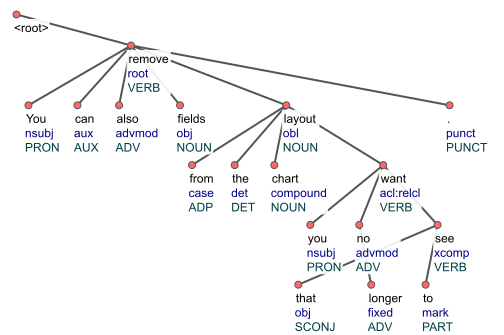
\includegraphics[scale=0.75]{img/nonproj-demo}
    \caption{Sample Non-projective Tree}
    Note: \textit{that} should be tagged as \texttt{PRON}, and not as \texttt{SCONJ}
    \label{fig:nonprojdemo}
\end{figure}

In the graph, notice the edge going from \textit{see} to \textit{that}. We can see that the edge crosses over another edge in order to link the two tokens. Informally, presence of such crossing edges in a tree makes it non-projective in nature.

\subsection{Related Terms and Formal Definition}

To define the concept of non-projective structures in a formal manner, we need to define a few notations. We use the same notations as used by \cite{mambriniNonProj}.

If a node \(j\) depends on a node \(i\), we call node \(j\) as a child node of \(i\) (also, \(i\) is parent node of \(j\)), represented as \(i \xrightarrow{} j\). We use \(i < j\) to denote the node \(i\) precedes node \(j\) in the word-order in tree \(T\). A node \(v\) lying in between the nodes \(i\) and \(j\) in the tree can be represented as \(v \in (i,j)\). Also, we use the notation \(v \in Subtree_{i}\) if node \(v\) is part of the subtree rooted at node \(i\). 

From \cite{Havelka}, we can define the condition of projectivity of a tree as follows:

\theoremstyle{definition}
\begin{definition}
\label{def:projectivity}
A given tree \(T\) is projective in nature iff
\begin{equation}
\label{eqn:projectivity}
    i \xrightarrow{} j \And v \in (i, j) \implies v \in Subtree_{i} \qquad \forall i, j, v \in T 
\end{equation}

If a given tree does not satisfy the above condition, it is said to be non-projective in nature. Furthermore, in case of non-projectivity, node \(v\) is said to be in gap, represented as \(v \in Gap_{i\leftrightarrow j}\). The double headed arrow signifies the nodes being considered irrelevant of their order of occurrence in the tree.
\end{definition}

\cite{mambriniNonProj}, in their work on \verb|grc|, highlight that the distribution of non-projective structures might be affected by genre distribution. In particular, poetic style is liable to contain more non-projective structures than prose. The claim about genre distribution affecting projectivity is also supported by \cite{nonprojgenre}, where they look at different genres (news and conversations) using different parameters to account for lack of non-projective structures in the conversational genre, than in news genre. %Although more research is needed on the topic, we try to base our experiments while restricting ourselves to the genre distributions that are more or less alike (cf. Section \ref{sec:nonproj_dataset} and discussion of \texttt{support treebanks}).

\subsection{Punctuation Induced Non-Projectivity}
\label{ssec:punct-nonproj}

A punctuation node can induce non-projectivity in either of the two ways as mentioned below:

\begin{enumerate}
    \item Non-projective attachment of a punctuation node.
    \item Non-projectivity caused by only punctuation node(s) in gap.
\end{enumerate}

According to UD guidelines, a punctuation node should be attached to the surrounding dependent unit. However, it is not always possible to identify the correct dependent where the node should be attached. Consider the following example from \verb|en|-lines UD v2.5 treebank, and the associated dependency tree in Figure \ref{fig:punct-nonproj}, with specific reference to the punctuation mark immediately following the token marked in bold. While the punctuation token could have been correctly marked to either of \textit{right} or \textit{said}, it is attached to \textit{'s} causing non-projectivity.

\begin{example}
That's \textbf{right}, said Quinn.
\end{example}

\begin{figure}[H]
    \centering
    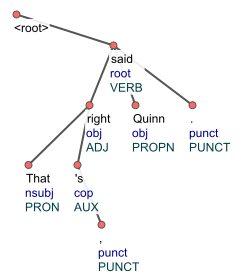
\includegraphics{img/punct-nonproj.png}
    \caption{Punctuation Node Attached Non-Projectively}
    \label{fig:punct-nonproj}
\end{figure}

Similarly, the punctuation node(s) can induce non-projectivity, by attaching itself to the wrong node. Consider the following example from \verb|en|-EWT UDv2.5 treebank, and the associated dependency tree in Figure \ref{fig:punct-nonproj2}, with specific reference to the punctuation mark immediately following the token in bold. A faulty association of this punctuation induces non-projectivity in another node.

\begin{example}
Analyst Team 1 : \textbf{Coach} : Lisa Gilette
\end{example}

\begin{figure}[H]
    \centering
    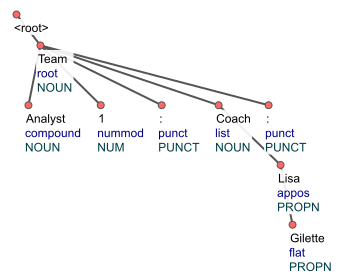
\includegraphics{img/punct-nonproj2.png}
    \caption{Punctuation Node Causing Non-Projectivity}
    \label{fig:punct-nonproj2}
\end{figure}

To summarise, we can say that a non-projective edge \(i \rightarrow j\) is a case of Punctuation Induced non-projectivty if any of the following conditions are met:

\begin{enumerate}
    \item Either of head (node \(i\)), or dependent (node \(j\)) is a punctuation node.
    \item The nodes in \(Gap(i, j)\) consist of \textbf{only} punctuation node(s).
\end{enumerate}

Projectivity in itself is a strict constraint for a multitude of natural languages. Therefore, there have been multiple relaxations that have been suggested over time on the strict constraint of projectivity. Appendix \ref{app:nonproj-relaxations} discusses some of these relaxations, and then lists in tabular form the statistics related to non-projectivity in different treebanks in UDv2.5 data.    % 06 pages
    \chapter{Related Work on Solutions to Identified Problems}
\label{chap:prev_research}

In this chapter, we discuss some of the solutions that have been proposed or used by the different researchers. The solutions discussed here are limited in the scope of the problems identified in the last chapter. It is important to note that there have been numerous papers studying the different treebanks in UD, and the set of problems encountered while changing the annotation from the guidelines for UDv1 to UDv2. While such research is helpful in pointing out cases where the annotating teams had difficulties during the conversion procedure, we do not discuss those references here, unless needed.

Before proceeding further, it is imperative to understand a subtle difference between error detection and inconsistency detection. If the errors are consistent in their distribution across the data, an inconsistency detection tool would fail in the discovery of such errors. In such case, the non erroneous part of the annotation would be the inconsistency and might be flagged as a false negative, provided the tool is biased towards the erroneous annotation. Any tool that tries to discover inconsistencies need not find such consistent error patterns. This is the major difference between error detection and inconsistency detection. Error mining methods are primarily based on detecting deviations from a standard clean reference (usually gold or platinum standard), and should be able to provide an analysis of the error patterns regardless of whether or not the error is present consistently. In this chapter, we use error mining and error detection interchangeably.

The rest of the chapter is organised as follows. We first discuss existing literature on inconsistency detection in Section \ref{sec:inconsistency-detection}, and the relevance of the literature to the problem identified in Section \ref{sec:harmony} on Annotation Consistency in Different Treebanks. We then focus on the literature relevant to error detection in Section \ref{sec:error-mining}.

\section{Annotation Consistency across Treebanks}
\label{sec:inconsistency-detection}

Owing to different annotation schemes for the different treebanks of a given language, there is no standard evaluation metric to compare the consistency of treebanks' annotation to each other to the best of our knowledge. 

One of the most commonly used approaches to find the inconsistencies in the annotation is to train a high quality parser or a tagger model on a given training data, and evaluating the cases where the prediction from the trained model differs from the annotation of the test data. This approach can also be extended by bootstrapping different trained models, with the majority consensus being compared against the available annotation. While this approach can point to individual inconsistencies, it does not say anything about the errors in the treebank. Furthermore, the different treebanks of the same language can have different annotation inconsistencies with the errors being consistent in their presence throughout. Additionally, the consistent errors in the different treebanks can be vastly different from each other as well.

To ascertain annotation quality of one or more treebanks, both inconsistency detection and error detection should be used. In case of individual treebanks, UD website\footnote{\url{universaldependencies.org}} shows against each treebank a metric score that is an approximation of the quality of the treebank. The metric is calculated heuristically\footnote{For more details on the associated heuristics, refer to \url{https://github.com/UniversalDependencies/tools/blob/master/evaluate_treebank.pl}}, depending on multiple factors like the number of genres present in the treebank, the score as provided by official UD validator\footnote{refer to \url{https://github.com/UniversalDependencies/tools/blob/master/validate.py}}, among others. When it comes to comparing annotation quality among multiple treebanks, there exist no metrics or tools to the best of our knowledge. However, some techniques have been used more often than others for such comparisons.

\subsection{Consistency in POS Annotation}
\label{ssec:inconsistency-detection-pos}

\cite{dickinson03a, dickinson03b} are the most well known pieces of work in detecting inconsistency in POS annotation, essentially forming the base of majority of inconsistency detection. The work focuses on finding a n-gram of tokens in the corpus that occurs in the same context (referred to as a variation nucleus) such that the different occurrences of the variation nucleus are annotated differently. Originally coined for continuous annotation\footnote{The annotation of the current token is based on the annotation of a contiguous token in word order. Discontinuous annotation implies the annotation of current token is dependent on another token that might not be contiguous in the word order, as in the case of dependency parsing.}, the method was eventually adapted to look for inconsistencies in discontinuous annotation as well \citep{dickinson05}.

\cite{korean} compare the POS annotation consistency for different treebanks in \verb|ko| by using the relative frequency of the individual POS tags. The authors also briefly mention the cause of the variation in distribution of the individual POS tags. While such analysis is slightly helpful in terms of drawing a comparison, it does not consider the interaction of different POS tags with each other. To illustrate such interactions, a n-gram based approach might be utilised. Even so, absence of \verb|SCONJ| tag in one treebank prevents the analysis with respect to other treebanks.

\subsection{Consistency in Dependency Annotation}
\label{ssec:inconsistency-detection-deprel}

The original method of using variation nuclei for continuous annotation as proposed by \cite{dickinson03a, dickinson03b} was extended for discontinuous annotation in \cite{dickinson05}, as mentioned earlier. By extending the method to discontinuous annotations, \citeauthor{dickinson05} were able to look at more patterns in TIGER corpus. Moreover, this meant that instead of looking at plain POS tags and identifying the variations therein, the words could now be looked at in order to generalize the context.

\cite{alonso2016universal} compared the treebanks for \verb|es| in UDv1.3 \citep{UDv1.3}. They assess the similarity of the different treebanks using dependency parsing. A high-efficiency parser was trained on one of the treebanks, and then tested on another. The idea was to notice the drop in LAS scores, and if the difference in scores was more than what was intuitive, the treebanks were marked as not similar enough. The same technique of evaluating the different treebanks for \verb|ru| against each other was also used in \cite{RussianTreebanks}. In their work spanning the different \verb|ru| treebanks in UD, \citeauthor{RussianTreebanks} also point out problems with individual treebanks. The problems pointed out therein can be used as a starting point to scout for patterns that are present across the different treebanks for the language. 

\cite{CLAS} proposed an evaluation metric called CLAS (Content-based LAS) score that disregard the punctuation and other functional nodes, evaluating LAS based on content words only. The change of evaluation metric from LAS to CLAS was meant as a way to give equal treatment to the languages with weak morphology and languages with strong morphology. For example, a single inconsistency in \verb|fi| will affect the parsing score more than a single inconsistency in \verb|en| owing to the differences in the extent of morphology used by the languages. The metric was evaluated as a secondary measure in CoNLL 2017 Shared Task \citep{CLAS_test}. The primary metric for the Shared Task was macro-averaged LAS score for the different languages. It was reported that there is no significant performance difference in parser performances when the evaluation metric was changed from macro-averaged LAS score to CLAS score.

An important point to note here is that the metrics LAS and CLAS are associated with the performance of parsers. The metric scores would be lower in case even when the parser is able to parse the data better than the manual annotation. The two metrics (and also unlabelled attached score or UAS) therefore cannot be relied upon for detection of the inconsistencies.

\cite{korean} compare the dependency annotation consistency among different treebanks in \verb|ko| by again focusing on the relative frequency of the dependency labels, offering reasons for the variation in distribution of the individual label. A dependency label is determined by the choice of the parent label as well, and thus the method of \citeauthor{korean} is of little help in flagging any inconsistencies.

\subsection{LISCA}
\label{ssec:lisca_soln}

\cite{lisca} used an unsupervised algorithm which attempts to find the inconsistencies in dependency annotation by building a statistical model on the data from a given reference corpus (ideally, a gold standard). This algorithm, called LISCA, creates a language model for the given dependency arcs, learning for each arc its probability of occurrence based on a subset of local and global attributes associated with the arc. The eventually created language model can then be used to rank the dependency arcs in another parsed corpus by their probability of occurrence. Figure \ref{fig:lisca_stats} shows graphically some of the features used by LISCA to calculate score for an arc.

\begin{figure}[H]
    \centering
    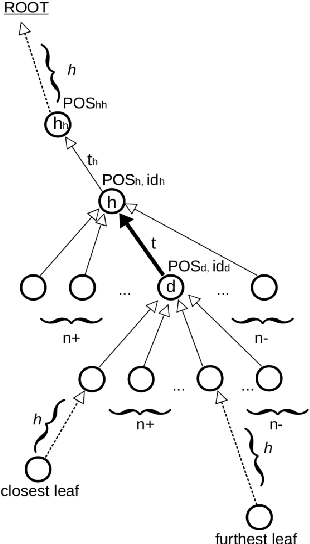
\includegraphics[scale=0.5]{img/lisca_stats.png}
    \caption[Features Used by LISCA to Calculate Plausibility Score for an Arc]{Features Used by LISCA to Calculate Plausibility Score for an Arc (marked in bold). Figure borrowed from \cite{alzetta2017dangerous}}
    \flushleft{Local Feature: Distance in terms of tokens between $d$ and $h$\\
    Local Feature: Associative strength linking grammatical categories $POS_{d}$ and $POS_{h}$\\
    Local Feature: POS of the head governor and type of syntactic dependency connecting it to $h$\\
    Global Feature: Distance of $d$ from the root of the tree\\
    Global Feature: Distance of $d$ from the closest or the most distant leaf node\\
    Global Feature: Number of siblings to the right of node $d$ in the linear order of the sentence\\
    Global Feature: Number of children to the left of node $d$ in the linear order of the sentence}
    \label{fig:lisca_stats}
\end{figure}

LISCA was used to identify the errors in newspaper section of Italian UD Treebank in \cite{alzetta2017dangerous}. In their work, they narrow the search space for the errors by binning the arcs according to the scores into 10 bins of equal size and an extra bin to include the extra cases. The bins were then manually inspected for errors, while concentrating on the last two (and the extra) bins containing the arcs with lowest scores. Analysing the data, 36\% of the arcs in the low ranking bins consisted of random errors, while the remaining ones were found to be systemic and recurrent errors (even in treebanks of different languages).

While the algorithm mentioned above successfully points out the arcs that are inconsistent in their annotation in the different datasets, it is sensitive to the genre of the data. The authors note that the data should ideally belong to the same register or genre for the algorithm to function at its best. While this is problematic because in some treebanks it is not possible to separate the data from different genres, there is also a possibility of unavailability of enough data in a particular genre (i.e. a single genre contributing in a very small manner to the size of the treebank).

Added to these difficulties is the difficulty of training the algorithm. The algorithm essentially needs to be trained on a gold standard data, from which it builds a statistical model that is used to generate the probability scores of a dependency arc. In case of languages with no high-quality parsers available or for low-resource languages, this poses a cold-start problem where we do not have the data to train the algorithm, and so the algorithm cannot be used at all.

We tried solving this problem of cold-start by using the method of \(k\)-fold cross validation (with varying values of \(k\)) in training the algorithm. We discuss the experiment in more detail in Chapter \ref{chap:lisca}.

\section{Error Mining Methods}
\label{sec:error-mining}

Error mining in treebanks can be done in multiple ways. There is a possibility of using hand-written rules, and scouting for the patterns in the relevant treebank. This manual approach works well for finding error typologies that are known beforehand. The other approach is to combine the statistical approach, with the manually defined rules \citep{ambati}. This method is referred to as heuristics-based search since it identifies a lot of patterns, which can then be used to look for errors in the data (in some cases, this can be done automatically). The last approach is automatic scouting for error patterns within the scope of the treebank, also known as automatic error mining.

\subsection{Automatic Error Mining Based on n-gram Approach}

\cite{boyd} first introduced the idea of error mining methods in dependency treebanks using variation nuclei, expanding on the idea of using n-grams based variation nuclei for discontinuous annotations from \cite{dickinson05}. This is often referred to as the first automatic error mining method in dependency treebanks.

\cite{de2017assessing} extended and evaluated the method proposed by \citeauthor{boyd}, in context of UD Treebanks for three languages (\verb|en|, \verb|fi|, \verb|fr|). The authors further extended the method to use word lemmas instead of simply using word forms, and also evaluate on the automatically annotated treebanks to identify more inconsistencies. The first extension of using lemmas works well for languages that are not too morphologically-rich (\verb|en|, \verb|fr|), but fails otherwise. The second extension is done at the cost of a drop in precision, but without a significant gain in recall.

The method proposed by \citeauthor{boyd} has an inherent problem instance of data sparseness. \cite{kook} implemented an algorithm based on n-grams and suspicion sharing across the n-grams by extending the methods of \cite{sagot} and \cite{noord}. Their approach however, relies on classifying each sentence within the results of a parsed corpus as a parsable or unparsable sentence. This classification of individual sentence needs to be done manually, and is therefore not optimal for large treebanks.

\newpage   % 04 pages
    \chapter{Estimating POS Annotation Consistency of Different Treebanks in a Language (Experiment 1)}
\label{chap:pos-harmony}

We introduced the problem of inter treebank POS annotation quality in Section \ref{sec:harmony} earlier, followed by a discussion of the literature relevant to the problem in Section \ref{ssec:inconsistency-detection-pos}. 

In this chapter, we propose a metric based on $KL_{cpos^3}$ metric \citep{klcpos3}, which in turn is based upon Kullback-Liebler Divergence (KL Divergence). 

We start by a short introduction to $KL_{cpos^3}$ metric and a definition of the proposed metric in Section \ref{sec:pos-harmony-definition}. We define our dataset for the experiments in this chapter in Section \ref{sec:pos-harmony-dataset}, followed by the metric values being listed for different treebanks in UDv2.5 \citep{UDv2.5} in Section \ref{sec:pos-harmony-scores}. The experiments are detailed in Section \ref{sec:pos-harmony-size} and Section \ref{sec:pos-harmony-genre}, with their results summarised in Section \ref{sec:pos-harmony-calculations}. We mark the treebanks as consistent or inconsistent in their POS annotation in Section \ref{sec:theta_pos_annotations}. The chapter concludes with a discussion on the metric in Section \ref{sec:pos-harmony-conclusion}.

\section{\texorpdfstring{$KL_{cpos^3}$}{KLcpos3} and Metric Definition}
\label{sec:pos-harmony-definition}

\cite{klcpos3} show that KL-Divergence score of POS trigrams can be effectively used for source selection for POS Tagging in a delexicalised cross-language model transfer scenario. In their approach, they are able to select effectively not just a singular source, but are also able to rank multiple sources by specifying weights to individual source in a multi-source transfer scenario. Computing the KL-Divergence on POS trigrams, they call the measure as $KL_{cpos^3}$, defined as follows:

\begin{definition}
\label{def:klcpos3}

\textbf{ }\\

\begin{equation}
\label{eqn:klcpos3}
\small KL_{cpos^3}(tgt, src) = \sum_{\forall cpos^3 \in tgt}^{}f_{tgt}(cpos^3)\log\frac{f_{tgt}(cpos^3)}{f_{src}(cpos^3)}
\end{equation}
where $cpos^3$ is a coarse POS tag trigram, and \\

\begin{align}
\label{eqn:cpos}
f(cpos^3) & = \nonumber f(cpos_{i-1}, cpos_{i}, cpos_{i+1}) \\ &= \frac{count(cpos_{i-1}, cpos_{i}, cpos_{i+1})}{\sum_{\forall cpos_{a,b,c}}{count(cpos_{a}, cpos_{b}, cpos_{c})}}
\end{align}
with $count_{src}(cpos^3) = 1$ for each unseen trigram.

\end{definition}

Intuitively, treebanks of the same language (despite the differences in the genres covered) should be better fit for single-source transfer than a treebank from another language. This is the primary motivation for using $KL_{cpos^3}$ (as defined for a single-source transfer scenario) to assess the annotation consistency among the treebanks of a language. However, $KL_{cpos^3}$ is a variant of KL-Divergence, and thus asymmetric, making it unfit in its original form for assessing annotation consistency symmetrically. We refer to the symmetric variant of the metric as $\theta_{pos}$ defined for the treebanks $A$ and $B$ as follows:

\begin{equation}
    \boxed{\theta_{pos}(A, B) = KL_{cpos^3}(A,B) + KL_{cpos^3}(B,A)}
\end{equation}
where $KL_{cpos^3}(P,Q)$ indicates $KL_{cpos^3}$ score of $Q$ as an estimator for $P$.

Since $KL_{cpos^3}$ is a non-negative divergence metric, so is $\theta_{pos}$. While either metric is numeric in nature, the $KL_{cpos^3}$ scores can be used as an estimator of quality in presence of an absolute gold standard. However, in absence of an absolute gold standard, the scores for the metric in different treebanks can not be compared directly. In such case (of lack of absolute gold standard), there should be an upper bound that needs to be placed on the $\theta_{pos}$ scores. As long as the $\theta_{pos}$ scores are lower than this upper bound, the considered pair of treebanks can be considered as harmonious in terms of their POS annotation. We call this upper bound as $\Theta_{pos}$. The metrics $\theta_{pos}$ and $\Theta_{pos}$ are linked together in the following definition.

\begin{definition}
\label{def:harmony}
Given two treebanks $A$ and $B$, we say the treebanks are in harmony with (or, are harmonious to) each other in terms of POS annotation, if the symmetric measure of their mutual divergence (given by $\theta_{pos}$) is less than or equal to a threshold (given by $\Theta_{pos}$). \\
    Mathematically, it can be represented as:
    \begin{align}
    \label{eq:pos_harmony}
        \Aboxed{\theta_{pos}(A, B) & = \nonumber KL_{cpos^3}(A,B) + KL_{cpos^3}(B,A)} \\
        &\leq \Theta_{pos}(A, B)
    \end{align}
    where $KL_{cpos^3}(P,Q)$ indicates $KL_{cpos^3}$ score of $Q$ as an estimator for $P$.
\end{definition}

Even though $\Theta_{pos}$ is a bound on the $\theta_{pos}$ metric, the former is essentially a property of the latter. For a given set of guidelines, and a given set of data, the upper bound value would need to be estimated often, albeit using the same technique. In the remaining chapter, we try to estimate the upper bound in a language-independent manner by looking at the influence of size of data, and the POS distribution in individual genres on $\theta_{pos}$ metric. While the methods that we shall discuss shortly can be applied for estimations across different guidelines and different set of data, care must be taken while estimating the upper bound for a new guideline (or even on different iterations of UD data). If the estimated value of $\Theta_{pos}$ is too large, we run the risk of saying the treebanks are harmonious even when they might not be. Also, if the value is too small, we could be overlooking at the effect of domain change and dataset size, to mistakenly announce the pair of treebanks as being non-harmonious to each other.

\section{Dataset}
\label{sec:pos-harmony-dataset}

UDv2.5 \citep{UDv2.5} contains 157 treebanks in 90 languages. There are multiple languages with more than one treebank, with some containing up to 6 treebanks. A list of all such languages, with the associated treebanks can be seen in Appendix \ref{app:multi_trees}. We list $\theta_{pos}$ scores of the different treebanks in different languages in the next section. In the listing of scores, small treebanks where the total number of sentences is less than 1 000 are not included.

As mentioned earlier, the treebanks in UD are assigned a score based on the system of checks run by the official UD validator. We want to estimate the $\Theta_{pos}$ scores to the best of our ability, and so, working with a pair of low quality treebanks would be the worst approach that can be undertaken. To that effect, we estimate the bounding score on treebanks with the ratings of at least 3.5 stars (out of 5 stars). The treebanks selected in this manner can be considered to be of high quality. The selection of high quality treebanks also enforces an important assumption, that the data within a singular treebank has been annotated consistently or that there are considerably lower number of annotation inconsistencies within the data in a treebank. The assumption would also imply that in a pair of considered treebanks, while the treebanks might not be annotated consistently with respect to each other, the individual treebanks are assumed to be internally consistent with respect to their annotation.

The assumption as mentioned above is a strict constraint, and might not always hold. An alternative assumption can be used in cases where the stricter version is not expected to hold. The relaxed version of the assumption assumes that the data belonging to one particular genre in a treebank would be annotated consistently throughout. This is a relaxation in the sense that given multiple genres in a treebank, the entire treebank might not be annotated consistently. However, the data in individual genres is annotated consistently. The experiments listed in this chapter work within the bound of these assumptions. 

\section{\texorpdfstring{$\theta_{pos}$}{theta\_pos} Scores for UDv2.5}
\label{sec:pos-harmony-scores}

\begin{minipage}{0.50\textwidth}
\subsection*{Languages with 2 Treebanks}
\begin{table}[H]
    \scalebox{0.90}{\begin{tabular}{|l|l|l|}
    \hline
    \textbf{Treebank1} & \textbf{Treebank2} & \textbf{$\theta_{pos}$} \\
    \hline
    \texttt{ar}-NYUAD & \texttt{ar}-PADT & 2.497\\
    \hline
    \texttt{es}-AnCora & \texttt{es}-GSD & 0.352\\
    \hline
    \texttt{et}-EDT & \texttt{et}-EWT & 0.413 \\
    \hline
    \texttt{fi}-FTB & \texttt{fi}-TDT & 1.195 \\
    \hline
    \texttt{gl}-CTG & \texttt{gl}-TreeGal & 0.714 \\
    \hline
    \texttt{grc}-Perseus & \texttt{grc}-PROIEL & 4.641 \\
    \hline
    \texttt{ja}-GSD & \texttt{ja}-BCCWJ & 0.951 \\
    \hline
    \texttt{ko}-GSD & \texttt{ko}-Kaist & 2.56 \\
    \hline
    \texttt{nl}-Alpino & \texttt{nl}-LassySmall & 0.664 \\
    \hline
    \texttt{pl}-LFG & \texttt{pl}-PDB & 0.623 \\
    \hline
    \texttt{pt}-Bosque & \texttt{pt}-GSD & 0.678 \\
    \hline
    \texttt{ro}-Nonstandard & \texttt{ro}-RRT & 1.233 \\
    \hline
    \texttt{sl}-SSJ & \texttt{sl}-SST & 2.405 \\
    \hline
    \texttt{sv}-LinES & \texttt{sv}-Talbanken & 0.443 \\
    \hline
    \texttt{tr}-GB & \texttt{tr}-IMST & 1.477 \\
    \hline
    \texttt{zh}-GSD & \texttt{zh}-HK & 1.958\\
    \hline
    \end{tabular}}
    \end{table}
    
    \subsection*{Languages with 3+ Treebanks}
    
    \begin{table}[H]
    \scalebox{0.90}{\begin{tabular}{|l|l|l|l|}
    \hline
    \texttt{cs} & \textbf{CAC} & \textbf{CLTT} & \textbf{FicTree} \\
    \hline
    \textbf{CLTT} & 1.453 & - & - \\
    \hline
    \textbf{FicTree} & 1.138 & 2.657 & - \\
    \hline
    \textbf{PDT} & 0.373 & 1.935 & 1.006 \\
    \hline 
    \end{tabular}}
    \end{table}
    
    % \vspace{1cm}
    \end{minipage}
    \hfill
    \begin{minipage}{0.48\textwidth}
    \subsection*{Languages with 3 Treebanks}
    \begin{table}[H]
    \begin{tabular}{|l|l|l|}
    \hline
    \texttt{de} & \textbf{GSD} & \textbf{HDT} \\
    \hline
    \textbf{HDT} & 0.49 & - \\
    \hline
    \textbf{LIT} & 1.383 & 1.1 \\
    \hline
    \end{tabular}
    \end{table}
    
    \begin{table}[H]
    \begin{tabular}{|l|l|l|}
    \hline
    \texttt{la} & \textbf{ITTB} & \textbf{Perseus} \\
    \hline
    \textbf{Perseus} & 1.106 & - \\
    \hline
    \textbf{PROIEL} & 3.763 & 3.901 \\
    \hline
    \end{tabular}
    \end{table}
    
    \begin{table}[H]
    \scalebox{0.90}{\begin{tabular}{|l|l|l|}
    \hline
    \texttt{no} & \textbf{Bokmaal} & \textbf{Nynorsk} \\
    \hline
    \textbf{Nynorsk} & 0.095 & - \\
    \hline
    \textbf{NynorskLIA} & 2.291 & 2.375 \\
    \hline
    \end{tabular}}
    \end{table}
    
    \begin{table}[H]
    \begin{tabular}{|l|l|l|}
    \hline
    \texttt{ru} & \textbf{GSD} & \textbf{SynTagRus} \\
    \hline
    \textbf{SynTagRus} & 0.567 & - \\
    \hline
    \textbf{Taiga} & 1.027 & 0.631 \\
    \hline
    \end{tabular}
    \end{table}
    \end{minipage}
    
    \begin{table}[H]
    \scalebox{0.80}{\begin{tabular}{|l|l|l|l|l|}
    \hline
    \texttt{en} & \textbf{EWT} & \textbf{GUM} & \textbf{LinES} & \textbf{ParTUT}\\
    \hline
    \textbf{GUM} & 0.26 & - & - & -\\
    \hline
    \textbf{LinES} & 0.407 & 0.455 & - & -\\
    \hline 
    \textbf{ParTUT} & 0.62 & 0.432 & 0.581 & -\\
    \hline 
    \textbf{ESL} & 0.592 & 0.799 & 0.564 & 0.823\\
    \hline 
    \end{tabular}}
    \end{table}
    
    \begin{table}[H]
    \scalebox{0.80}{\begin{tabular}{|l|l|l|l|l|l|}
    \hline
    \texttt{fr} & \textbf{FQB} & \textbf{GSD} & \textbf{ParTUT} & \textbf{Sequoia} & \textbf{Spoken}\\
    \hline
    \textbf{GSD} & 1.582 & - & - & - & -\\
    \hline
    \textbf{ParTUT} & 1.942 & 0.683 & - & - & -\\
    \hline
    \textbf{Sequoia} & 1.693 & 0.248 & 0.524 & - & -\\
    \hline
    \textbf{Spoken} & 3.644 & 3.089 & 2.599 & 2.732 & -\\
    \hline
    \textbf{FTB} & 2.226 & 0.379 & 0.7 & 0.272 & 3.507\\
    \hline
    \end{tabular}}
    \end{table}
    
    \begin{table}[H]
    \scalebox{0.80}{\begin{tabular}{|l|l|l|l|l|}
    \hline
    \texttt{it} & \textbf{ISDT} & \textbf{ParTUT} & \textbf{VIT} & \textbf{PoSTWITA}\\
    \hline
    \textbf{ParTUT} & 0.133 & - & - & - \\
    \hline
    \textbf{VIT} & 0.121 & 0.194 & - & -\\
    \hline
    \textbf{PoSTWITA} & 1.67 & 1.478 & 1.764 & - \\
    \hline
    \textbf{TWITTIRO} & 1.501 & 1.376 & 1.594 & 0.347 \\
    \hline
    \end{tabular}}
    \end{table}

\section{Dataset Size and \texorpdfstring{$\theta_{pos}$}{theta\_pos}}
\label{sec:pos-harmony-size}

$KL_{cpos^{3}}(tgt, src)$ is defined on distributions of trigrams found in $tgt$ and $src$. The calculated metric scores should therefore be affected by the presence or absence of the POS trigrams. The presence/absence of POS trigrams can similarly affect the calculations of $\theta_{pos}$ metric scores. In this part of the experiment, we use k-fold cross validation to check the effect of presence/absence of POS trigrams in the data. We use k-fold cross validation here as it allows us to check how the calculated scores are affected based on the size of the data alone, and also to frame an association of the scores with the presence/absence of POS trigrams, if any. 

The presence/absence of data from different genres can affect the calculation of $\theta_{pos}$ scores. In order to discount such effect, the entire data used for the analysis should belong to the same genre. For this experiment, we used \verb|cs|-PDT (rated 4.5/5 stars) and \verb|et|-EDT (rated 4/5 stars) treebanks. The motivation behind the selection of languages is primarily the difference in their language families. Additionally, the two treebanks contain a large number of sentences belonging to the \textit{news} genre, making it easier for the data to be studied across multiple k-fold runs with different k-values. Table \ref{tab:pos-harmony-size-datasize} lists the sentences counts associated to the considered genres in either treebank.

\begin{table}[H]
    \centering
    \begin{tabular}{|c|l|l|}
        \hline
        \textbf{Language} & \textbf{Genre} & \textbf{Sentences}\\
        \hline
        \texttt{cs} & News & 53 075 \\
        \hline
        \texttt{et} & News & 13 557 \\
        \hline
    \end{tabular}
    \caption{Sentence Counts in \texttt{cs}-PDT and \texttt{et}-EDT Treebanks}
    \label{tab:pos-harmony-size-datasize}
\end{table}


To check the effect of data size on $\theta_{pos}$ metric, we ran k-fold cross validation on the data from the aforementioned treebank in the following manner:

\begin{enumerate}
    \item Concatenate the different splits of the treebank together before downsampling the concatenated data to a fixed number of instances.
    \item For different predetermined k-values, the downsampled data is split into k folds. In each fold, the $\theta_{pos}$ scores are calculated between the fold's splits.
    \item In each fold, we try to estimate the projection of trigram distribution from the test set for the fold, onto the training set for the fold. Essentially, the training set in a fold corresponds to $src$, while the test set corresponds to $tgt$. We try to calculate coverage of different POS trigrams in each fold. The coverage is calculated by counting the number of trigrams common to both $src$ and $tgt$, expressed as a percentage of the total number of trigrams in $tgt$.
\end{enumerate}

The methodology as stated above is listed for a single repetition over a single treebank. To get a better estimation of the values, the method was repeated 100 times each for both the treebanks. In each repetition, the seed values were uniquely selected so as to get different downsamples every time. Table \ref{tab:pos-harmony-size} lists the number of instances the treebank was downsampled to, and the considered k values for the downsampled data. The table also lists the $\theta_{pos}$ scores and coverage scores for each fold. The scores are averaged over the 100 repetitions for each k-value, with the standard deviation (sd) also mentioned therein.

\begin{table}[H]
    \centering
    \begin{tabular}{|c|c||c|l|l|}
        \hline
        \textbf{Language} & \textbf{Downsample} & \textbf{k value} & \textbf{$\theta_{pos}$ Score} & \textbf{Coverage (in \%)}\\
        \hline
        \hline
        \multirow{7}{*}{\texttt{cs}} & \multirow{7}{*}{50000} & 5 & 0.021 $\pm$ 0.001 & 83.904 $\pm$ 0.563\\
        & & 10 & 0.037 $\pm$ 0.001 & 75.457 $\pm$ 0.602\\
        & & 20 & 0.069 $\pm$ 0.002 & 66.138 $\pm$ 0.656\\
        & & 50 & 0.161 $\pm$ 0.005 & 52.754 $\pm$ 0.832\\
        & & 100 & 0.304 $\pm$ 0.011 & 42.368 $\pm$ 0.843\\
        & & 250 & 0.663 $\pm$ 0.03 & 29.353 $\pm$ 0.864\\
        & & 500 & 1.092 $\pm$ 0.063 & 20.802 $\pm$ 1.021\\
        \hline
        \hline
        \multirow{8}{*}{\texttt{et}} & \multirow{8}{*}{12000} & 4 & 0.064 $\pm$ 0.002 & 76.15 $\pm$ 0.807\\
        & & 6 & 0.087 $\pm$ 0.003 & 69.739 $\pm$ 0.957\\
        & & 8 & 0.109 $\pm$ 0.004 & 65.237 $\pm$ 0.83\\
        & & 12 & 0.155 $\pm$ 0.006 & 58.667 $\pm$ 1.032\\
        & & 16 & 0.2 $\pm$ 0.007 & 54.124 $\pm$ 1.029\\
        & & 24 & 0.286 $\pm$ 0.012 & 47.77 $\pm$ 1.046\\
        & & 48 & 0.52 $\pm$ 0.02 & 37.096 $\pm$ 0.947\\
        & & 120 & 1.038 $\pm$ 0.053 & 24.485 $\pm$ 1.151\\
        \hline
    \end{tabular}
    \caption[$\theta_{pos}$ and Coverage of POS Trigram Scores ($\pm$ sd) Averaged over 100 Different Runs to Highlight the Effect of Size Disparity]{$\theta_{pos}$ and Coverage of POS Trigram Scores ($\pm$ sd) Averaged over 100 Different Runs to Highlight the Effect of Size Disparity. The values in the $\theta_{pos}$ and Coverage columns are the representative scores for the k-value, selected from the scores of individual runs such that the score is statistically equal to scores of more than 50\% of the runs in the fold. The statistical value is calculated at 95\% confidence using One Sampled t-test.}
    \label{tab:pos-harmony-size}
\end{table}

Looking at the scores for the two languages, there is a clear negative correlation between coverage and $\theta_{pos}$ score. Coverage of different POS trigrams is, however, dependent upon the size of the datasets being compared. In case of a really small dataset, the number of different POS trigrams or even the total number of POS trigrams is not comparable.

Figures \ref{fig:trigram-PDT} and \ref{fig:trigram-EDT} consist of two graphs each. The graphs show how the number of (i) distinct POS trigrams, and (ii) total number of POS trigrams is affected by a change in the dataset size. While the first graph in each figure shows the variability across the entire downsampled data (50000 sentences in \texttt{cs} in Figure \ref{fig:trigram-PDT}, and 12000 sentences in \texttt{et} in Figure \ref{fig:trigram-EDT}); the second graph zooms in on the progression over 2000 sentences.

\begin{figure}[H]
    \centering
    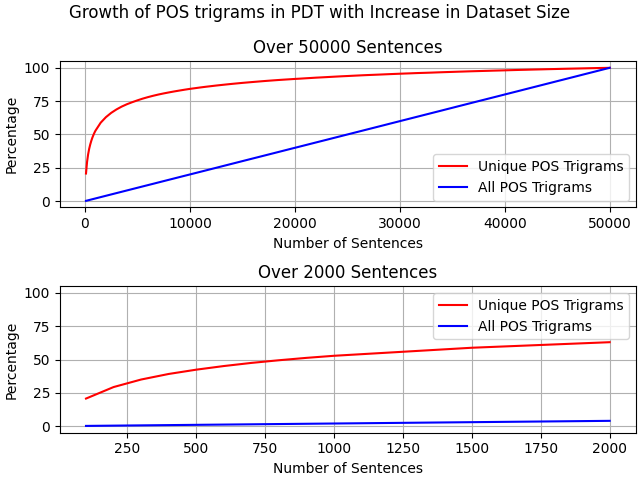
\includegraphics[scale=0.75]{img/trigram-stats-PDT.png}
    \caption{Growth of POS Trigrams in PDT with Increase in Dataset Size}
    \label{fig:trigram-PDT}
\end{figure}

\begin{figure}[H]
    \centering
    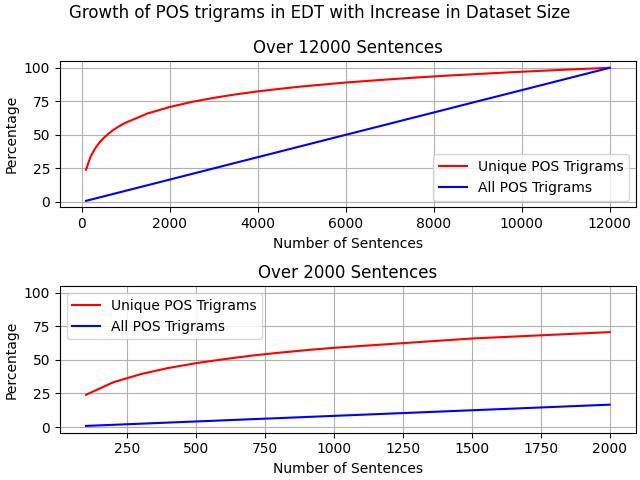
\includegraphics[scale=0.75]{img/trigram-stats-EDT.png}
    \caption{Growth of POS Trigrams in EDT with Increase in Dataset Size}
    \label{fig:trigram-EDT}
\end{figure}

As can be seen from the figures, the growth pattern is similar across both the languages. We can see that in case of a considerably small dataset size, the POS trigrams can not be considered as representative of those present in the entire dataset. We claim that for a proper estimation of the annotation consistency in two datasets belonging to the same genre, either dataset requires at least 400 sentences ($\approx 40\%$ of unique POS trigrams) for the estimation to be reliable. The minimum limitation on the size of the datasets ensures that the distribution of POS trigrams in either dataset is not skewed because of a small size.

\begin{claim}
Data across two datasets $A, B$ can be compared iff \\
\begin{equation*}
    \boxed{size(A) \geq 400 \And size(B) \geq 400}
\end{equation*}
\label{claim:pos_size_init}
\end{claim}

where $size(X)$ refers to the size of dataset $X$ in terms of the number of sentences

Table \ref{tab:counts-ar} shows the average sentence length of sentences in different treebanks for \verb|ar|. If we consider equal number of sentences from either of \verb|ar|-NYUAD or \verb|ar|-PADT treebanks and compare the POS annotation consistency with \verb|ar|-PUD treebanks, the total number of syntactic words differ by a factor of almost 2. 

\begin{table}[H]
    \centering
    \begin{tabular}{|l|l|l|l|}
    \hline
    \textbf{Counts} & \texttt{ar}-NYUAD & \texttt{ar}-PADT & \texttt{ar}-PUD \\
    \hline
    Syntactic Words & 738889 & 282384 & 20751 \\
    Sentences & 19738 & 7664 & 1000\\
    \hline
    \textbf{Average} & 37.434 & 36.845 & 20.751\\
    \hline
    \end{tabular}
    \caption[Average Sentence Lengths in \texttt{ar} Treebanks]{Average Sentence Lengths in \texttt{ar} Treebanks. In \texttt{es}, the token \textbf{v\'amonos} (Let's go) is split into 2 syntactic words \textbf{vamos} (go-\textit{1P-Pl.}) and \textbf{nos} (\textit{1P.-Pl.}) for annotation.}
    \label{tab:counts-ar}
\end{table}

When calculating the $\theta_{pos}$ scores for a set of treebanks, the average sentence length in either treebank should also be taken into account. It makes sense to limit the size of the datasets in consideration not in absolute terms, but also in reference to each other. Keeping this in mind, we update Claim \ref{claim:pos_size_init} to account for the average sentence length in Claim \ref{claim:pos_size}.

\begin{claim}
Data across two datasets $A, B$ can be compared iff \\
\begin{equation}
\label{eqn:size_constraint}
    \boxed{size(A) \geq 400 \And Avg(A) \geq Avg(B) \implies size(B) \cdot \frac{Avg(B)}{Avg(A)} \geq 400}
\end{equation}
\label{claim:pos_size}
\end{claim}

where 
\begin{enumerate}
    \item $Avg(X) = \frac{Total Syntactic Words(X)}{size(X)}$ is the average sentence length in dataset $X$
    \item $size(X)$ refers to the number of sentences in dataset $X$
\end{enumerate}

From the results of the data in Table \ref{tab:pos-harmony-size}, when the test split is composed of 500 instances ($k=100$ for \texttt{cs}; $k=24$ for \texttt{et}), the $\theta_{pos}$ metric is $\approx 0.3$. Considering that the larger $k$-values in either dataset do not satisfy the condition in Equation \ref{eqn:size_constraint}, we use the values as per the aforementioned $k$-values to estimate the maximal value for $\theta_{pos}$ when there is a size variance in the datasets.

As mentioned earlier, the treebanks in the consideration are ranked high in their quality check. Considering that some treebanks might not have such high quality of annotation, we allow some room for the change in $\theta_{pos}$ metric. 

If the datasets $A$, $B$ contain data from the same genre, and the size of the datasets is comparable (as per Equation \ref{eqn:size_constraint}), the upper limit on the $\theta_{pos}$ score can be specified as per Equation \ref{eqn:theta_pos_size_limit}.

\begin{equation}
    \boxed{\theta_{pos}(A,B) \leq \Theta_{pos}(A,B) = 0.5}
\label{eqn:theta_pos_size_limit}
\end{equation}

\section{Genre Distribution and \texorpdfstring{$\theta_{pos}$}{theta\_pos}}
\label{sec:pos-harmony-genre}

There can be significant difference(s) between genres in terms of syntactic annotations that are typical of the genre. While this difference is best exhibited across treebanks containing data from different genres, it can also be exhibited within a given treebank. The problem of music genre classification in speech data has been studied in detail, with different audio similarity metrics being proposed as well (cf. \cite{music1, music2}, among others). In the written data, while there has been some research on the study of inter-genre variations for language acquisition \citep{genre-acquisition1}, the classification of genres in textual corpus is identified mainly by the source of data.

\subsection{Relevant Literature on Textual Genres and Their Similarity}

In \cite{biber2}, a line of distinction is drawn between between text type and genre as the basis of classification of texts. While the former is `defined and distinguished on the basis of systematic nonlinguistic criteria', the latter is `defined on the basis of strictly linguistic criteria (similarities in the use of cooccuring linguistic features)' \cite[p.~39]{biber2}. In \cite{biber}, the different genres in \verb|en| are studied in different dimensions, focusing on one dimension at a time. The dimensions are a group of factors that associate the different features of a discourse, and are as listed in Table \ref{tab:dimensions-genres}. In the same work, the author notes that a given genre can contain multiple sub-genres which may or may not be internally coherent to each other \cite[p.~170]{biber}, and that no dimension in itself can attribute to the similarity or dissimilarity of the genres. In a later study that seeked to understand the variations of the genres based on these identified dimensions across 4 languages, the author notes that `even when defined at a high level of generality, parallel registers are more similar cross-linguistically than are disparate registers within a single language' \cite[p.~279]{biberbook}.

\begin{table}[H]
    \scalebox{0.9}{\begin{tabular}{|c|l|l|}
    \hline
    \textbf{S.No.} & \textbf{Dimension Name} & \textbf{Characteristic of Dimension} \\
    \hline
    \hline
    1. & \textbf{Involved vs Informational Production} & interactional, affective, involved \\
     & & purposes, associated with \\
     & & strict real-time production and \\
     & & comprehension constraints\\
    \hline
    2. & Narrative vs Non-Narrative Concerns & primary narrative purpose\\
    \hline
    3. & \textbf{Explicit vs Situation-Dependent} & identifies referents fully and \\
     & \textbf{Reference} & explicitly through relativization\\
    \hline
    4. & Overt Expression of Persuasion & speaker's expression of own \\
     & & point of view or with\\
     & & argumentative styles \\
     & & to persuade the addressee\\
    \hline
    5. & Abstract vs Non-Abstract Information & highly abstract and technical \\
    & & informational focus\\
    \hline
    6. & \textbf{On-Line Information Elaboration} & production under highly \\
    & & constrained conditions where \\
    & & information is presented \\
    & & in relatively loose, fragmented\\
    & & manner\\
    \hline
    \end{tabular}}
    \caption[Identified Dimensions for Comparison of Genres in \cite{biber}]{Identified Dimensions for Comparison of Genres. The characteristic of individual dimensions is as found in \cite[p.~115]{biber}. Dimension 5 on `Abstract vs Non-Abstract Information' is noted to be not universal across all languages \cite[p.~278]{biberbook}}
    \label{tab:dimensions-genres}
\end{table}

The dimensions marked in bold in Table \ref{tab:dimensions-genres} can be summarised under the notion of \textit{deep formality}, as coined in \cite{formality1}. \citeauthor{formality1} are able to classify linguistic constructions into different genres according to the measurement of their formality, based on a numerical measure of formality. The numerical measure, however doesn't account for all the dimensions marked in bold, but mainly to the first dimension on `Involved vs Informational Production'. The formality of a construction was numerically calculated in terms of F-measure (formality measure), as defined in Equation \ref{eqn:formality}. \cite{formality2} discovered that a numerical I-measure (informality measure, needed for working with Web2.0 data, given in Equation \ref{eqn:informality}) combined with F-measure worked better in identification of formality levels in data than when either of the measure was used on its own.

\begin{align}
    \text{F-measure} &= \textstyle{\frac{f_{noun} + f_{adjective} + f_{preposition} + f_{article} - f_{pronoun} - f_{verb} - f_{adverb} - f_{interjection} + 100}{2}} \label{eqn:formality}\\
    \text{I-measure} &= (f_{mistyped} + f_{interjection} + f_{emoticon}) * 100 \label{eqn:informality}
\end{align}
where $f_{A}$ represents frequency of $A$.

In our experiment, we tried to experiment with a combination of F-measure and I-measure, as well as with the measures by themselves. Considering that the absolute frequency would be dependent on the size of the database, the measure scores were computed in terms of relative frequencies. However, we found no correlation between $\theta_{pos}$ scores between two genres, with their F-measure or I-measure scores or a combination of the two. % 05 pages on Preface to theta_POS
    \section{Dataset Size and \texorpdfstring{$\theta_{pos}$}{theta\_pos}}
\label{sec:pos-harmony-size}

$KL_{cpos^{3}}(tgt, src)$ is defined on distributions of trigrams found in $tgt$ and $src$. The calculated metric scores should therefore be affected by the presence or absence of the POS trigrams. The presence/absence of POS trigrams can similarly affect the calculations of $\theta_{pos}$ metric scores. In this part of the experiment, we use k-fold cross validation to check the effect of presence/absence of POS trigrams in the data. We use k-fold cross validation here as it allows us to check how the calculated scores are affected based on the size of the data alone, and also to frame an association of the scores with the presence/absence of POS trigrams, if any. 

The presence/absence of data from different genres can affect the calculation of $\theta_{pos}$ scores. In order to discount such effect, the entire data used for the analysis should belong to the same genre. For this experiment, we used \verb|cs|-PDT (rated 4.5/5 stars) and \verb|et|-EDT (rated 4/5 stars) treebanks. The motivation behind the selection of languages is primarily the difference in their language families. Additionally, the two treebanks contain a large number of sentences belonging to the \textit{news} genre, making it easier for the data to be studied across multiple k-fold runs with different k-values. Table \ref{tab:pos-harmony-size-datasize} lists the sentences counts associated to the considered genres in either treebank.

\begin{table}[H]
    \centering
    \begin{tabular}{|c|l|l|}
        \hline
        \textbf{Language} & \textbf{Genre} & \textbf{Sentences}\\
        \hline
        \texttt{cs} & News & 53 075 \\
        \hline
        \texttt{et} & News & 13 557 \\
        \hline
    \end{tabular}
    \caption{Sentence Counts in \texttt{cs}-PDT and \texttt{et}-EDT Treebanks}
    \label{tab:pos-harmony-size-datasize}
\end{table}


To check the effect of data size on $\theta_{pos}$ metric, we ran k-fold cross validation on the data from the aforementioned treebank in the following manner:

\begin{enumerate}
    \item Concatenate the different splits of the treebank together before downsampling the concatenated data to a fixed number of instances.
    \item For different predetermined k-values, the downsampled data is split into k folds. In each fold, the $\theta_{pos}$ scores are calculated between the fold's splits.
    \item In each fold, we try to estimate the projection of trigram distribution from the test set for the fold, onto the training set for the fold. Essentially, the training set in a fold corresponds to $src$, while the test set corresponds to $tgt$. We try to calculate coverage of different POS trigrams in each fold. The coverage is calculated by counting the number of trigrams common to both $src$ and $tgt$, expressed as a percentage of the total number of trigrams in $tgt$.
\end{enumerate}

The methodology as stated above is listed for a single repetition over a single treebank. To get a better estimation of the values, the method was repeated 100 times each for both the treebanks. In each repetition, the seed values were uniquely selected so as to get different downsamples every time. Table \ref{tab:pos-harmony-size} lists the number of instances the treebank was downsampled to, and the considered k values for the downsampled data. The table also lists the $\theta_{pos}$ scores and coverage scores for each fold. The scores are averaged over the 100 repetitions for each k-value, with the standard deviation (sd) also mentioned therein.

\begin{table}[H]
    \centering
    \begin{tabular}{|c|c||c|l|l|}
        \hline
        \textbf{Language} & \textbf{Downsample} & \textbf{k value} & \textbf{$\theta_{pos}$ Score} & \textbf{Coverage (in \%)}\\
        \hline
        \hline
        \multirow{7}{*}{\texttt{cs}} & \multirow{7}{*}{50000} & 5 & 0.021 $\pm$ 0.001 & 83.904 $\pm$ 0.563\\
        & & 10 & 0.037 $\pm$ 0.001 & 75.457 $\pm$ 0.602\\
        & & 20 & 0.069 $\pm$ 0.002 & 66.138 $\pm$ 0.656\\
        & & 50 & 0.161 $\pm$ 0.005 & 52.754 $\pm$ 0.832\\
        & & 100 & 0.304 $\pm$ 0.011 & 42.368 $\pm$ 0.843\\
        & & 250 & 0.663 $\pm$ 0.03 & 29.353 $\pm$ 0.864\\
        & & 500 & 1.092 $\pm$ 0.063 & 20.802 $\pm$ 1.021\\
        \hline
        \hline
        \multirow{8}{*}{\texttt{et}} & \multirow{8}{*}{12000} & 4 & 0.064 $\pm$ 0.002 & 76.15 $\pm$ 0.807\\
        & & 6 & 0.087 $\pm$ 0.003 & 69.739 $\pm$ 0.957\\
        & & 8 & 0.109 $\pm$ 0.004 & 65.237 $\pm$ 0.83\\
        & & 12 & 0.155 $\pm$ 0.006 & 58.667 $\pm$ 1.032\\
        & & 16 & 0.2 $\pm$ 0.007 & 54.124 $\pm$ 1.029\\
        & & 24 & 0.286 $\pm$ 0.012 & 47.77 $\pm$ 1.046\\
        & & 48 & 0.52 $\pm$ 0.02 & 37.096 $\pm$ 0.947\\
        & & 120 & 1.038 $\pm$ 0.053 & 24.485 $\pm$ 1.151\\
        \hline
    \end{tabular}
    \caption[$\theta_{pos}$ and Coverage of POS Trigram Scores ($\pm$ sd) Averaged over 100 Different Runs to Highlight the Effect of Size Disparity]{$\theta_{pos}$ and Coverage of POS Trigram Scores ($\pm$ sd) Averaged over 100 Different Runs to Highlight the Effect of Size Disparity. The values in the $\theta_{pos}$ and Coverage columns are the representative scores for the k-value, selected from the scores of individual runs such that the score is statistically equal to scores of more than 50\% of the runs in the fold. The statistical value is calculated at 95\% confidence using One Sampled t-test.}
    \label{tab:pos-harmony-size}
\end{table}

Looking at the scores for the two languages, there is a clear negative correlation between coverage and $\theta_{pos}$ score. Coverage of different POS trigrams is, however, dependent upon the size of the datasets being compared. In case of a really small dataset, the number of different POS trigrams or even the total number of POS trigrams is not comparable.

Figures \ref{fig:trigram-PDT} and \ref{fig:trigram-EDT} consist of two graphs each. The graphs show how the number of (i) distinct POS trigrams, and (ii) total number of POS trigrams is affected by a change in the dataset size. While the first graph in each figure shows the variability across the entire downsampled data (50000 sentences in \texttt{cs} in Figure \ref{fig:trigram-PDT}, and 12000 sentences in \texttt{et} in Figure \ref{fig:trigram-EDT}); the second graph zooms in on the progression over 2000 sentences.

\begin{figure}[H]
    \centering
    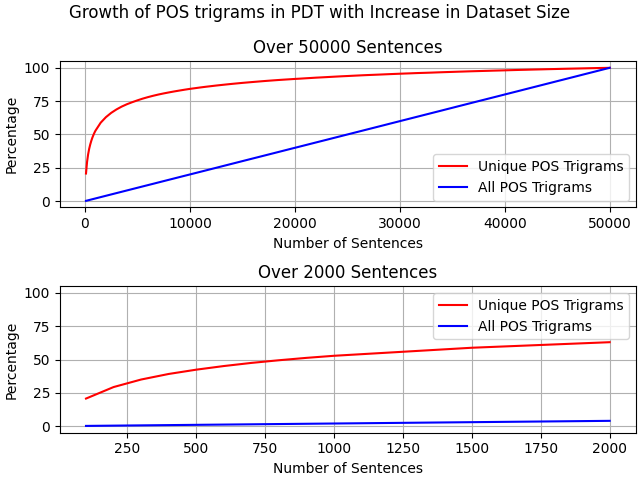
\includegraphics[scale=0.75]{img/trigram-stats-PDT.png}
    \caption{Growth of POS Trigrams in PDT with Increase in Dataset Size}
    \label{fig:trigram-PDT}
\end{figure}

\begin{figure}[H]
    \centering
    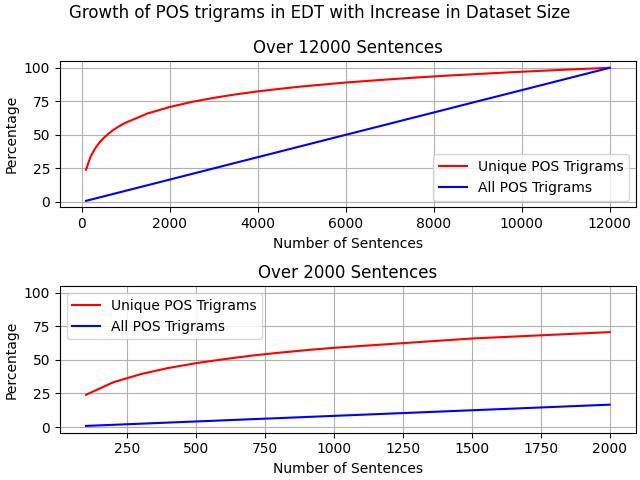
\includegraphics[scale=0.75]{img/trigram-stats-EDT.png}
    \caption{Growth of POS Trigrams in EDT with Increase in Dataset Size}
    \label{fig:trigram-EDT}
\end{figure}

As can be seen from the figures, the growth pattern is similar across both the languages. We can see that in case of a considerably small dataset size, the POS trigrams can not be considered as representative of those present in the entire dataset. We claim that for a proper estimation of the annotation consistency in two datasets belonging to the same genre, either dataset requires at least 400 sentences ($\approx 40\%$ of unique POS trigrams) for the estimation to be reliable. The minimum limitation on the size of the datasets ensures that the distribution of POS trigrams in either dataset is not skewed because of a small size.

\begin{claim}
Data in a given genre can be compared across two datasets $A, B$ iff \\
\begin{equation*}
    \boxed{size(A) \geq 400 \And size(B) \geq 400}
\end{equation*}
\label{claim:pos_size_init}
\end{claim}

where $size(X)$ refers to the size of dataset $X$ in terms of the number of sentences

Table \ref{tab:counts-ar} shows the average sentence length of sentences in different treebanks for \verb|ar|. If we consider equal number of sentences from either of \verb|ar|-NYUAD or \verb|ar|-PADT treebanks and compare the POS annotation consistency with \verb|ar|-PUD treebanks, the total number of syntactic words differ by a factor of almost 2. 

\begin{table}[H]
    \centering
    \begin{tabular}{|l|l|l|l|}
    \hline
    \textbf{Counts} & \texttt{ar}-NYUAD & \texttt{ar}-PADT & \texttt{ar}-PUD \\
    \hline
    Syntactic Words & 738889 & 282384 & 20751 \\
    Sentences & 19738 & 7664 & 1000\\
    \hline
    \textbf{Average} & 37.434 & 36.845 & 20.751\\
    \hline
    \end{tabular}
    \caption[Average Sentence Lengths in \texttt{ar} Treebanks]{Average Sentence Lengths in \texttt{ar} Treebanks. In \texttt{es}, the token \textbf{v\'amonos} (Let's go) is split into 2 syntactic words \textbf{vamos} (go-\textit{1P-Pl.}) and \textbf{nos} (\textit{1P.-Pl.}) for annotation.}
    \label{tab:counts-ar}
\end{table}

When calculating the $\theta_{pos}$ scores for a set of treebanks, the average sentence length in either treebank should also be taken into account. It makes sense to limit the size of the datasets in consideration not in absolute terms, but also in reference to each other. Keeping this in mind, we update Claim \ref{claim:pos_size_init} to account for the average sentence length in Claim \ref{claim:pos_size}.

\begin{claim}
Data in a given genre can be compared across two datasets $A, B$ iff \\
\begin{equation}
\label{eqn:size_constraint}
    \boxed{size(A) \geq 400 \And Avg(A) \geq Avg(B) \implies size(B) \geq Avg(A) \cdot 400}
\end{equation}
\label{claim:pos_size}
\end{claim}

where 
\begin{enumerate}
    \item $Avg(X) = \frac{Total Syntactic Words(X)}{size(X)}$ is the average sentence length in dataset $X$
    \item $size(X)$ refers to the size of dataset $X$ in terms of the number of sentences
\end{enumerate}

From the results of the data in Table \ref{tab:pos-harmony-size}, when the test split is composed of 500 instances ($k=100$ for \texttt{cs}; $k=24$ for \texttt{et}), the $\theta_{pos}$ metric is $\approx 0.3$. Considering that the larger $k$-values in either dataset do not satisfy the condition in Equation \ref{eqn:size_constraint}, we use the values as per the aforementioned $k$-values to estimate the maximal value for $\theta_{pos}$ when there is a size variance in the datasets.

As mentioned earlier, the treebanks in the consideration are ranked high in their quality check. Considering that some treebanks might not have such high quality of annotation, we allow some room for the change in $\theta_{pos}$ metric. We can set up the limit on the $\theta_{pos}$ metric with respect to dataset size change as in Equation \ref{eqn:theta_pos_size_limit}, with datasets $A$, $B$ containing data from same genre, and subjected to condition as in Equation \ref{eqn:size_constraint}.

\begin{equation}
    \boxed{\theta_{pos}(A,B) \leq \Theta_{pos}(A,B) = 0.5}
\label{eqn:theta_pos_size_limit}
\end{equation}

\newpage % 05 pages on tuning theta_POS for size variation
\subsection{Inter-Genre Similarity}

\verb|pl|-LFG treebank in UDv2.5 (rated 4 stars on a scale of 5 stars) contains data from 8 different genres\footnote{For understanding of what genre category involves exactly what kind of data, refer to the github page of the treebank at \url{https://github.com/UniversalDependencies/UD_Polish-LFG}}. The sentence counts of different genres are shown in Table \ref{tab:genre_pl}. We club together the different kind of data in \textit{spoken} genre, as one. We remove \textit{academic}, \textit{blog} and \textit{legal} data from our consideration owing to a considerably low number of sentences. Table \ref{tab:genre_fi} shows the genre distribution in UDv2.5 \texttt{fi}-TDT data. In this case, the data with source as \textit{europarl} and university articles (\textit{uni\_articles}) is kept separate from other categories. The genres we work with are marked in bold in the table. 

\begin{table}[H]
    \centering
    \begin{tabular}{|l|c|l|}
        \hline
        \textbf{Genre} & \textbf{Sentence Count} & \textbf{Avg()}\\
        \hline
        \hline
        \textbf{fiction} & 7 252 & 7.124 \\
        \textbf{news} & 6 744 & 8.401\\
        \textbf{nonfiction} & 1 273 & 7.719\\
        \textbf{social} & 526 & 6.977\\
        \textbf{spoken} & 1253 & 6.047\\
        academic & 51 & 8.118\\
        blog & 136 & 7.772\\
        legal & 11 & 9.273\\ 
        \hline
    \end{tabular}
    \caption{Genre Distribution in UDv2.5 \texttt{pl}-LFG treebank}
    \label{tab:genre_pl}
\end{table}

\begin{table}[H]
    \centering
    \begin{tabular}{|l|c|l|}
        \hline
        \textbf{Genre} & \textbf{Sentence Count} & \textbf{Avg()}\\
        \hline
        \hline
        \textbf{fiction} & 2739 & 11.981\\
        \textbf{wiki} & 2269 & 14.049\\
        \textbf{grammar} & 2002 & 8.48\\
        \textbf{blog} & 1781 & 12.533\\
        \textbf{legal} & 1141 & 20.968\\
        \textbf{news} & 3064 & 13.026\\ 
        europarl & 1082 & 18.441\\
        uni\_articles & 1058 & 13.261\\
        \hline
    \end{tabular}
    \caption{Genre Distribution in UDv2.5 \texttt{fi}-TDT treebank}
    \label{tab:genre_fi}
\end{table}

In order to establish that the different genres are annotated consistently within themselves, we downsample the dataset for each genre in \texttt{fi}-TDT treebank to 900 sentences. On this downsampled data, we perform 2-fold cross validation split, and calculate the $\theta_{pos}$ score for the splits. We repeat this calculation 100 times, such that the data is downsampled differently each time, as per a different seed value. Table \ref{tab:genre_all_kfold} shows the calculated $\theta_{pos}$ scores averaged over 100 different runs.

\begin{table}[H]
    \centering
    \begin{tabular}{|l|l|l|}
        \hline
        \textbf{Genres} & \textbf{$\theta_{pos}$} ($\pm$ sd) & $\Theta_{pos}$\\
        \hline
        \textbf{fiction} & 0.316 $\pm$ 0.015 & 0.5\\
        \textbf{wiki} & 0.3 $\pm$ 0.017 & 0.5\\
        \textbf{grammar} & 0.427 $\pm$ 0.021 & 0.5\\
        \textbf{blog} & 0.332 $\pm$ 0.017 & 0.5\\
        \textbf{legal} & 0.216 $\pm$ 0.035 & 0.5\\
        \textbf{news} & 0.286 $\pm$ 0.015 & 0.5\\
        europarl & 0.233 $\pm$ 0.017 & 0.5\\
        uni\_articles & 0.3 $\pm$ 0.014 & 0.5\\
        \hline
    \end{tabular}
    \caption{$\theta_{pos}$ ($\pm$ sd) Scores Averaged Over 100 Different Runs for Different Genres in UDv2.5 \texttt{fi}-TDT Treebank To Show Intra-Genre Annotation Consistency}
    \label{tab:genre_all_kfold}
\end{table}

As can be seen from Table \ref{tab:genre_all_kfold}, the different genres in the treebank are internally consistent in their annotation, as per the constraint in Equation \ref{eqn:size_constraint}.

We start the inter-genre analysis by downsampling the datasets for different genres in the dataset. Table \ref{tab:downsample_genre} shows the count of sentences in the downsampled data from each genre. Each genre is downsampled to the number of instances such that the condition as specified in Equation \ref{eqn:size_constraint} is satisfied.

\begin{table}[H]
    \centering
    \begin{tabular}{|c|l|c|c|}
        \hline
        \textbf{Language} & \textbf{Genre (X)} & \textbf{Downsampled To} & \textbf{$size(X) \cdot \frac{Avg(X)}{Avg(A)}$}\\
         \hline
         & fiction & 500 & 424 \\
         & \textbf{news} & 500 & 500 \\
        \texttt{pl} & nonfiction & 500 & 459 \\
         & social & 500 & 415 \\
         & spoken & 600 & 432 \\
        \hline
         & fiction & 1000 & 571 \\
         & wiki & 1000 & 670 \\
        \texttt{fi} & grammar & 1000 & 404 \\
         & blog & 1000 & 598 \\
         & \textbf{legal} & 1000 & 1000 \\
         & news & 1000 & 621 \\
        \hline
    \end{tabular}
    \caption[Counts of Sentences for Different Genres in Downsampled Data from UDv2.5 \texttt{fi}-TDT and \texttt{pl}-LFG Treebanks]{Counts of Sentences for Different Genres in Downsampled Data from UDv2.5 \texttt{fi}-TDT and \texttt{pl}-LFG Treebanks. $A$ in $Avg(A)$ in the third column refers to the genre with the highest number of average words per sentence in each language, marked in bold.}
    \label{tab:downsample_genre}
\end{table}

For downsampled data from each genre, we compute the $\theta_{pos}$ scores. We present the scores for \texttt{pl} data in Table \ref{tab:inter_genre-pl} and for \texttt{fi} data in Table \ref{tab:inter_genre-fi}. It is worth noting that for most genres, the $\Theta_{pos}$ constraint as employed in Equation \ref{eqn:size_constraint} isn't enough, as $\theta_{pos}$ frequently surpasses the imposed limit of $0.5$.

\begin{table}[H]
\centering
\scalebox{1.0}{
    \begin{tabular}{|l|l|l|l|l|}
    \hline
    \textbf{Genres} & \textbf{news} & \textbf{nonfiction} & \textbf{social} & \textbf{spoken}\\
    \hline
    \textbf{fiction} & 0.754 $\pm$ 0.047 & 0.556 $\pm$ 0.028 & 0.726 $\pm$ 0.032 & 1.059 $\pm$ 0.047\\
    \textbf{news} & - & 0.55 $\pm$ 0.032 & 0.906 $\pm$ 0.044 & 1.53 $\pm$ 0.071\\
    \textbf{nonfiction} & - & - & 0.624 $\pm$ 0.027 & 1.285 $\pm$ 0.046\\
    \textbf{social} & - & - & - & 1.178 $\pm$ 0.033\\
    \hline
\end{tabular}}
\caption{$\theta_{pos}$ Scores ($\pm$ sd) Averaged over 100 runs for Inter-Genre Analysis in Downsampled UDv2.5 \texttt{pl}-LFG Data}
\label{tab:inter_genre-pl}
\end{table}

\begin{table}[H]
\centering
\scalebox{0.85}{
    \begin{tabular}{|l|l|l|l|l|l|}
    \hline
    \textbf{Genres} & \textbf{blog} & \textbf{grammar} & \textbf{wiki} & \textbf{legal} & \textbf{news}\\
    \hline
    \textbf{fiction} & 0.356 $\pm$ 0.014 & 0.47 $\pm$ 0.019 & 1.552 $\pm$ 0.041 & 1.559 $\pm$ 0.04 & 1.323 $\pm$ 0.044\\
    \textbf{blog} & - & 0.504 $\pm$ 0.018 & 1.307 $\pm$ 0.042 & 1.328 $\pm$ 0.026 & 1.113 $\pm$ 0.043\\
    \textbf{grammar} & - & - & 1.166 $\pm$ 0.041 & 1.554 $\pm$ 0.036 & 0.888 $\pm$ 0.035\\
    \textbf{wiki} & - & - & - & 1.229 $\pm$ 0.032 & 0.473 $\pm$ 0.021\\
    \textbf{legal} & - & - & - & - & 1.078 $\pm$ 0.026\\
    \hline
\end{tabular}}
\caption{$\theta_{pos}$ Scores ($\pm$ sd) Averaged over 100 runs for Inter-Genre Analysis in Downsampled UDv2.5 \texttt{fi}-TDT Data}
\label{tab:inter_genre-fi}
\end{table}

We attempted to associate the $\theta_{pos}$ scores across two genres based on if the genre belonged to spoken discourse, or from textual medium. However, as can be seen from the tables above, the scores can not be estimated on the basis of such distinction.

Looking at the data in the tables above, the maximal $\theta_{pos}$ score of $1.559$ is computed between \textit{legal} and \textit{fiction} categories. We hypothesise that a combination of F-score metric with a metric on `Narrative vs Non-Narrative Concerns' can be used to explain such high score. However, there exists no numeric metric to compute a genre's score on its `Narrative vs Non-Narrative Concerns' to the best of our knowledge. We therefore, are unable to associate the upper limit on $\theta_{pos}$ scores with respect to individual genres.

However, we can estimate a general upper bound. We allow some room for change in $\theta_{pos}$ score owing to high quality of annotation as while accounting for variability of dataset size change. With that in mind, we frame the general upper bound on $\theta_{pos}$ scores between genre $x$ in dataset $A$ (written as $A_{x}$) and genre $y$ in dataset $B$ (written as $B_{y}$) as in Equation \ref{eqn:theta_pos_genre_limit}, given below:

\begin{equation}
    \boxed{\theta_{pos}(A_{x}, B_{y}) \leq \Theta_{pos}(A_{x}, B_{y}) = 2.0}
\label{eqn:theta_pos_genre_limit}
\end{equation}
\newpage
\subsection{Combination of Genres}
\label{ssec:genres_combo}

In the previous section, we looked at how the $\theta_{pos}$ score changes when data from one genre is compared against another. In this subsection, we study how the different genres in combination with each other affect the $\theta_{pos}$ scores.

We denoted the set of genres in treebank $X$ as $G_{X}$. Given two treebanks $A$ and $B$ with at least one different genre, the different genres in the two treebanks $G_{A}$ and $G_{B}$ can be either of the three cases as shown in Figure \ref{fig:GA and GB interactions}.


\begin{figure}[H]
    \begin{subfigure}{.45\textwidth}
        \centering
        \begin{tikzpicture}[]
            \def\firstcircle{(-1.2,0) coordinate (a) circle (2cm)}
            \def\secondcircle{(-1.2,0) coordinate (b)  circle (1.5cm)}
                \begin{scope}
            \clip \secondcircle;
                \end{scope}
            \draw \firstcircle node[text=black,above] {$G_{A}$};
            \draw \secondcircle;
            \node (c) [above] at (current bounding box.north -| b) {$G_{B}$};
            % \node at (c -| b) {$G_{B}$};
        \end{tikzpicture}
        \caption{Case 1: $G_{A} \subseteq G_{B}$}
        \label{fig:case 1 ga gb}
    \end{subfigure}
    \begin{subfigure}{.5\textwidth}
        \centering
        \begin{tikzpicture}[]
            \def\firstcircle{(-1.2,0) coordinate (a) circle (2cm)}
            \def\secondcircle{(1.2,0) coordinate (b)  circle (2cm)}
                \begin{scope}
            \clip \secondcircle;
                \end{scope}
            \draw \firstcircle;
            \draw \secondcircle;
            \node (c) [above] at (current bounding box.north -| a) {$G_{A}$};
            \node at (c -| b) {$G_{B}$};
        \end{tikzpicture}
        \caption{Case 2: $G_{A} \not \subseteq G_{B}$; $G_{A} \cap G_{B} \neq \phi$}
        \label{fig:case 2 ga gb}
    \end{subfigure}
    \newline
    \begin{subfigure}{\textwidth}
        \centering
        \begin{tikzpicture}[]
            \def\firstcircle{(-3,0) coordinate (a) circle (2cm)}
            \def\secondcircle{(3,0) coordinate (b)  circle (2cm)}
                \begin{scope}
            \clip \secondcircle;
                \end{scope}
            \draw \firstcircle;
            \draw \secondcircle;
            \node (c) [above] at (current bounding box.north -| a) {$G_{A}$};
            \node at (c -| b) {$G_{B}$};
        \end{tikzpicture}
        \caption{Case 3: $G_{A} \not \subseteq G_{B}$; $G_{A} \cap G_{B} = \phi$}
        \label{fig:case 3 ga gb}
    \end{subfigure}
    \caption{Interaction of Genres in Treebanks $A$ and $B$, such that $\vert G_{A} \vert \leq \vert G_{B} \vert$}
    \label{fig:GA and GB interactions}
\end{figure}

To see how the $\theta_{pos}$ scores are affected in either of the cases, we perform the following experiment on UDv2.5 \texttt{pl}-LFG data.

\begin{enumerate}
    \item Downsample the number of sentences in \textit{fiction} and \textit{news} genres to 2000 sentences each. Using 2-fold cross-validation, split the downsampled into 2 halves. We refer to one half as \textit{base} set for the genre, and the other as the \textit{test} set for the genre, each containing 1000 sentences.
    \item Downsample the number of sentences in \textit{spoken} genre to 1000 sentences.
    \item Concatenate the downsampled \textit{spoken} data and the \textit{test} set from the other genres. Refer to this dataset as \textit{all\_genres}.
        \begin{equation*}
            \textit{all\_genres} = \textit{spoken} + \textit{fiction\_test} + \textit{news\_test}
        \end{equation*}
    \item Combine the \textit{test} sets to result in \textit{news\_fiction\_test} set.
        \begin{equation*}
            \textit{news\_fiction\_test} = \textit{news\_test} + \textit{fiction\_test}
        \end{equation*}
    \item Combine the \textit{base} sets to result in \textit{news\_fiction\_base} set.
        \begin{equation*}
            \textit{news\_fiction\_base} = \textit{news\_base} + \textit{fiction\_base}
        \end{equation*}
    \item Combine the downsampled \textit{spoken} data with either \textit{test} set to result in \textit{spoken\_genre\_test} data, where \textit{genre} is a placeholder for either of \textit{fiction} or \textit{news}.
        \begin{align*}
            \textit{spoken\_news\_test} & = \textit{spoken} + \textit{news\_test}\\
            \textit{spoken\_fiction\_test} &= \textit{spoken} + \textit{fiction\_test}
        \end{align*}
    \item For Case 1, we study the change in $\theta_{pos}$ score when the data as mentioned in Table \ref{tab:case1_genre} are compared against each other.
        \begin{table}[H]
            \centering
            \begin{tabular}{|c|c|}
                \hline
                \textbf{$G_{A}$} & \textbf{$G_{B}$} \\
                \hline
                $G_{news\_base} = \{news\}$ & $G_{news\_fiction\_test} = \{news, fiction\}$\\
                $G_{news\_base} = \{news\}$ & $G_{spoken\_news\_test} = \{spoken, news\}$\\
                $G_{news\_base} = \{news\}$ & $G_{all\_genres} = \{news, fiction, spoken\}$\\
                \hline
                $G_{fiction\_base} = \{fiction\}$ & $G_{news\_fiction\_test} = \{news, fiction\}$\\
                $G_{fiction\_base} = \{fiction\}$ & $G_{spoken\_fiction\_test} = \{spoken, fiction\}$\\
                $G_{fiction\_base} = \{fiction\}$ & $G_{all\_genres} = \{news, fiction, spoken\}$\\
                \hline
                $G_{news\_fiction\_base} = \{news, fiction\}$ & $G_{all\_genres} = \{news, fiction, spoken\}$\\
                \hline
            \end{tabular}
            \caption{Datasets Compared when $G_{A} \subset G_{B}$ and $\vert G_{A} \vert < \vert G_{B} \vert$}
            \label{tab:case1_genre}
        \end{table}
    \item For Case 2, we study the change in $\theta_{pos}$ score when the data as mentioned in Table \ref{tab:case2_genre} are compared against each other.
        \begin{table}[H]
            \centering
            \begin{tabular}{|c|c|}
                \hline
                \textbf{$G_{A}$} & \textbf{$G_{B}$} \\
                \hline
                $G_{news\_fiction\_base} = \{news, fiction\}$ & $G_{spoken\_news\_test} = \{spoken, news\}$\\
                $G_{news\_fiction\_base} = \{news, fiction\}$ & $G_{spoken\_fiction\_test} = \{spoken, fiction\}$\\
                \hline
            \end{tabular}
            \caption{Datasets Compared when $G_{A} \not \subseteq G_{B}$; $G_{A} \cap G_{B} \neq \phi$ and $\vert G_{A} \vert \leq \vert G_{B} \vert$}
            \label{tab:case2_genre}
        \end{table}
    \item For Case 3, we study the combinations as listed in Table \ref{tab:case3_genre}.
        \begin{table}[H]
            \centering
            \begin{tabular}{|c|c|}
                \hline
                \textbf{$G_{A}$} & \textbf{$G_{B}$} \\
                \hline
                $G_{news\_base} = \{news\}$ & $G_{spoken\_fiction\_test} = \{spoken, fiction\}$\\
                $G_{fiction\_base} = \{fiction\}$ & $G_{spoken\_news\_test} = \{spoken, news\}$\\
                $G_{spoken} = \{spoken\}$ & $G_{news\_fiction\_test} = \{news, fiction\}$\\
                \hline
            \end{tabular}
            \caption{Datasets Compared when $G_{A} \not \subseteq G_{B}$; $G_{A} \cap G_{B} = \phi$ and $\vert G_{A} \vert \leq \vert G_{B} \vert$}
            \label{tab:case3_genre}
        \end{table}
    \item We also calculate $\theta_{pos}$ scores for each \textit{base} and \textit{test} sets with each other, and with \textit{spoken} data, to better know how the scores are being impacted.
    \item We repeat all the above steps 100 times, each with a different seed value to result in differently downsampled data. We present the calculated scores averaged over 100 runs for different cases in Tables \ref{tab:case1_genre-results} - \ref{tab:case3_genre-results}. In the tables, the `Average' column contains the average of means from the preceding columns.
\end{enumerate}

\begin{table}[H]
    \centering
    \begin{tabular}{|c|c|c|c|c|}
        \hline
         & \textit{news\_test} & \textit{fiction\_test} & Average & \textit{news\_fiction\_test}\\
        \hline
        \textit{news\_base} & 0.257 ± 0.01 & 0.646 ± 0.034 & 0.452 & 0.304 ± 0.016 \\
        \textit{fiction\_base} & 0.64 ± 0.034 & 0.278 ± 0.013 & 0.46 & 0.348 ± 0.019 \\
        \hline
    \end{tabular}%
    \vspace{5mm}
    \begin{tabular}{|c|c|c|c|c|}
        \hline
         & \textit{news\_test} & \textit{spoken} & Average & \textit{spoken\_news\_test}\\
        \hline
        \textit{news\_base} & 0.257 ± 0.01 & 1.503 ± 0.049 & 0.88 & 0.489 ± 0.022\\
        \hline
    \end{tabular}%
    \vspace{5mm}
    \begin{tabular}{|c|c|c|c|c|}
        \hline
         & \textit{fiction\_test} & \textit{spoken} & Average & \textit{spoken\_fiction\_test}\\
        \hline
        \textit{fiction\_base} & 0.278 ± 0.013 & 0.99 ± 0.036 & 0.63 & 0.41 ± 0.018\\
        \hline
    \end{tabular}%
    \vspace{5mm}
    \scalebox{0.8}{\begin{tabular}{|c|c|c|c|c|c|}
        \hline
         & \textit{news\_test} & \textit{fiction\_test} & \textit{spoken} & Average & \textit{all\_genres}\\
        \hline
        \textit{news\_base} & 0.257 ± 0.01 & 0.646 ± 0.034 & 1.503 ± 0.049 & 0.802 & 0.463 ± 0.022\\
        \textit{fiction\_base} & 0.64 ± 0.034 & 0.278 ± 0.013 & 0.99 ± 0.036 & 0.64 & 0.351 ± 0.014\\
        \textit{news\_fiction\_base} & 0.3 ± 0.015 & 0.351 ± 0.021 & 1.144 ± 0.035 & 0.6 & 0.247 ± 0.011\\
        \hline
    \end{tabular}}
    \caption{Case 1}
    \label{tab:case1_genre-results}
\end{table}

\begin{table}[H]
    \centering
    \scalebox{0.9}{\begin{tabular}{|c|c|c|c|c|}
        \hline
         & \textit{spoken} & \textit{news\_test} & Average & \textit{spoken\_news\_test}\\
        \hline
        \textit{news\_base} & 1.503 ± 0.049 & 0.257 ± 0.01 & 0.88 & 0.489 ± 0.022\\
        \textit{fiction\_base} & 0.99 ± 0.036 & 0.64 ± 0.034 & 0.81 & 0.499 ± 0.02\\
        \textit{news\_fiction\_base} & 1.144 ± 0.035 & 0.3 ± 0.015 & 0.7 & 0.498 ± 0.023\\
        \hline
    \end{tabular}}%
    \vspace{5mm}
    \scalebox{0.9}{\begin{tabular}{|c|c|c|c|c|}
        \hline
         & \textit{spoken} & \textit{fiction\_test} & Average & \textit{spoken\_fiction\_test}\\
        \hline
        \textit{news\_base} & 1.503 ± 0.049 & 0.646 ± 0.034 & 1.075 & 0.854 ± 0.036\\
        \textit{fiction\_base} & 0.99 ± 0.036 & 0.278 ± 0.013 & 0.63 & 0.41 ± 0.018\\
        \textit{news\_fiction\_base} & 1.144 ± 0.035 & 0.351 ± 0.021 & 0.747 & 0.498 ± 0.023\\
        \hline
    \end{tabular}}
    \caption{Case 2}
    \label{tab:case2_genre-results}
\end{table}

\begin{table}[H]
    \centering
    \begin{tabular}{|c|c|c|c|c|}
        \hline
         & \textit{spoken} & \textit{fiction\_test} & Average & \textit{spoken\_fiction\_test}\\
        \hline
        \textit{news\_base} & 1.503 ± 0.049 & 0.646 ± 0.034 & 1.075 & 0.854 ± 0.036\\
        \hline
    \end{tabular}%
    \vspace{5mm}
    \begin{tabular}{|c|c|c|c|c|}
        \hline
         & \textit{spoken} & \textit{news\_test} & Average & \textit{spoken\_news\_test}\\
        \hline
        \textit{fiction\_base} & 0.99 ± 0.036 & 0.64 ± 0.034 & 0.81 & 0.499 ± 0.02\\
        \hline
    \end{tabular}%
    \vspace{5mm}
    \begin{tabular}{|c|c|c|c|c|}
        \hline
         & \textit{news\_test} & \textit{fiction\_test} & Average & \textit{news\_fiction\_test}\\
        \hline
        \textit{spoken} & 1.493 ± 0.048 & 0.987 ± 0.034 & 1.24 & 1.138 ± 0.03\\
        \hline
    \end{tabular}
    \caption{Case 3}
    \label{tab:case3_genre-results}
\end{table}

From the tables, it can be observed that the decomposition of a treebank into its constituent genres forms the first basis for the combination of the different genres. Once the individual genres have been identified and checked for the inter-generic $\theta_{pos}$ scores, the overall metric score is less than the average of the metric scores calculated for individual pair of genres in the treebank(s). Upon a closer inspection, it was discovered that when there are multiple genres present in the treebank, the $\theta_{pos}$ metric score is dominated by the POS trigrams that are typical of the language, and the genre-specific POS trigrams become more and more obscure.

Assuming treebanks $A$ and $B$ can be split into their constituent genres such that $G_{A} = \{A_{1}, A_{2}, ... , A_{i}\}$ and $G_{B} = \{B_{1}, B_{2}, ... , B_{j}\}$, the overall limit on the $\theta_{pos}(A, B)$ score can be specified as in Equation \ref{eqn:theta_pos_combo_limit}.

\begin{equation}
    \boxed{\theta_{pos}(A, B) \leq \Theta_{pos}(A, B) = Average(\theta_{pos}(A_{x}, B_{y}))} \hspace{5mm} \forall [A_{x} \in G_{A}; B_{y} \in G_{B}]
\label{eqn:theta_pos_combo_limit}
\end{equation}

\section{Framing Overall \texorpdfstring{$\Theta_{pos}$}{Theta\_pos} Limit}
\label{sec:pos-harmony-calculations}

We studied the effects of size and genre variation in treebanks in the previous sections. It was stated earlier that in order for two datasets to be compared, they should satisfy the condition as mentioned in Equation \ref{eqn:size_constraint} (restated below).

\begin{equation}
\boxed{size(A) \geq 400 \And Avg(A) \geq Avg(B) \implies size(B) \cdot \frac{Avg(B)}{Avg(A)} \geq 400} \tag{\ref{eqn:size_constraint}}
\end{equation}

 where

\begin{enumerate}
    \item $Avg(X) = \frac{Total Syntactic Words(X)}{size(X)}$ is the average sentence length in dataset $X$
    \item $size(X)$ refers to the number of sentences in dataset $X$
\end{enumerate}

For given datasets of the same genre such that the datasets satisfy the condition in Equation \ref{eqn:size_constraint} above, the upper limit on the $\theta_{pos}$ metric score for the datasets to be deemed as consistent in their annotation is specified in Equation \ref{eqn:theta_pos_size_limit} (restated below).

\begin{equation}
\boxed{\theta_{pos}(A,B) \leq \Theta_{pos}(A,B) = 0.5}  \tag{\ref{eqn:theta_pos_size_limit}}
\end{equation}

The different genres possible in a treebank can be analysed in two aspects. The first aspect looks at the formality and informality level within a genre, given by the genre's F-measure and I-measure respectively. While the original terms were defined on the basis of the frequency of the different POS tags, we worked with normalised frequency counts of the different POS tags to make the measures comparable against different treebanks, irrespective of their size. 

\textbf{Add stuff here}

For the different treebanks that are present in two treebanks, the limit on the $\theta_{pos}$ metric can be determined by the average score of the $\theta_{pos}$ scores calculated by Equation ref{eqn:theta-limit-genre} between different genres present in the treebanks, such that the dataset from the genres satisfy the equation \ref{eqn:theta_pos_combo_limit}.
% There are a large number of genres that are not covered in our approach. However, we can come up with a theoretical limit nonetheless. We can describe our coverage of genres in 3 broad categories, viz. print media (\textit{fiction}, \textit{news}, \textit{nonfiction}), social media (\textit{blog}, \textit{social}) and spoken data (\textit{spoken}). There exists an overlap between the categories. However, any genre that is not included can almost always be classified within the realm of the categories defined above. It is important to note that the categories should be considered as points in the continuous range, and not as discreet ones in themselves. From there, we can establish the upper limits on the variability of \(\theta_{POS}\) score as in Table \ref{tab:thetapos_genre}.

% \begin{table}[h]
%     \centering
%     \begin{tabular}{|c|c|c|}
%     \hline
%     \textbf{Category 1} & \textbf{Category 2} & \textbf{Limit} \\
%     \hline
%     Print & Social & 0.8 \\
%     Print & Spoken & 1.4 \\
%     Social & Spoken & 1.4 \\
%     \hline
%     \end{tabular}
%     \caption{Limits on \(\theta_{POS}\) for Genre-based Disparity}
%     \label{tab:thetapos_genre}
% \end{table}

% \section{Discussion and Conclusion}
% \label{sec:pos-harmony-conclusion}

% \subsection{Unaccounted Factors}
% \subsubsection{Out of Vocabulary Words}

% The metric \(\theta_{pos}\) uses POS trigrams to compute the divergence of the annotation. Since the metric is delexicalised, the concept of out-of-vocabulary (OOV) words does not make sense in the calculation of the metric score. In case of either treebank being annotated (semi-)automatically by a POS tagger, the improper annotation of OOV words can affect the scores negatively.

% In UD tagset, \verb|X| tag is reserved for words such that they can not be categorised under any of the other POS. While it is recommended to be used in a restricted manner\footnote{\url{https://universaldependencies.org/u/pos/X.html}}, the tag can exhibit itself abundantly depending on the origin source of the data, with the genres containing Web2.0 data being especially susceptible.

% For most treebanks, the influence of OOV words should be minimal. Nonetheless, care must be taken when the \verb|X| tag is present in the trigrams of either of the treebanks.

% \subsection{Conclusion}

% In practice, it is not always possible to get an estimate of the annotation quality of individual treebanks. Neither of the aforementioned assumptions can be made in such cases. If either of the treebanks in a considered pair can be estimated for quality, the other treebank can be compared for a similar annotation quality. However, like in the x 
% \textbf{ELABORATE}
% \textbf{blah}
    \chapter{\texttt{conj\_head}: Head Identification Error in Coordinating Conjunctions (Experiment 2)}
\label{chap:conj_head}

As discussed in Section \ref{sssec:conj_head}, \texttt{conj\_head} refers to the head identification error for a given coordinating conjunction. This error is characterized by the coordinating conjunction being linked to the previous conjunct (in UDv1), rather than by the next conjunct (in UDv2). We define the problem statement as identification of correct head for a given coordinating conjunction. In our treatment of the problem in this section, we start with a glance through some of the observations on the problem in Section \ref{ssec:conj_head_observations}, allowing us to define our effective dataset in Section \ref{ssec:conj_head_dataset}. We elaborate on our proposed solution to the problem, and the explanation of the algorithm used in the experiment in Section \ref{ssec:conj_head_experiment} and \ref{ssec:conj_head_algorithm} respectively. We finally evaluate the experiment in Section \ref{ssec:conj_head-results}.

\section{Observations About Problem Statement}
\label{ssec:conj_head_observations}

Identification of coordinating conjunctions, and separating them from subordinating conjunctions is a problem in itself and warrants a separate discussion of its own. Combined with the possible association of multiple deprels to a particular POS tag (cf. Section \ref{sssec:conj_deprels_association}), it is necessary to explicitly put a constraint on the instances to be considered during the scope of this experiment. To that effect, we identify coordinating conjunctions with their POS tag marked as \verb|CCONJ|, and the deprel as \verb|cc|. We disregard other deprels associated with the POS \verb|CCONJ| in the current context, effectively limiting the number of instances to be considered. In other words, we assume that any token that is POS tagged as \verb|CCONJ| and with deprel as \verb|cc| is a coordinating conjunction and that every coordinating conjunction is tagged in this manner, without exceptions. While the assumption is not fool proof and is not guaranteed to always hold, a deviation from this assumption would be a parsing/tagging error, and is therefore not relevant to this experiment.

In the following subsections, we take a look at some of the quirks associated with the problem. Through these quirks, we seek to (i) discover triggers that can help us in identification of problematic instances; and (ii) identify possible problems that we can run into while handling the aforementioned problematic instances. Throughout the rest of the experiment, we shall employ the following terminology:

\begin{enumerate}
    \item The terms ``coordinating conjunction", and ``conjunction" are used interchangeably.
    \item The term ``coordination" refers to the entire construction that consists of conjuncts, and (typically one) conjunction.
    \item In the following example, the coordination (\textit{Jack and Jill}) is marked in bold, while the conjunction (\textit{and}) is marked in italic.
    \begin{example}
    \textbf{Jack \textit{and} Jill} went up the hill to fetch a pail of water.
    \end{example}
\end{enumerate}

\subsection{Direction of Dependency}

Owing to the change in associated dependency from right-headed to left-headed\footnote{\url{https://universaldependencies.org/v2/coordination.html\#left--vs-right-headed-coordination}}, the intuitive approach to the problem at hand is to first look for the direction of dependency for a given coordinating conjunction token, identifying the instances where the attachment is right-headed. However, the identification of the correct direction can be non-trivial if worked in a language-independent manner. Consider the case of \verb|sa|, and how it differs from \verb|en|, as in Example \ref{examp:conj_sa}. In \verb|en|, the coordinating conjunction occurs in between the different conjuncts. In the given example for \verb|sa|, the conjunction is linked with the last conjunct in a form that is typical of the language. The word of interest in the example is marked explicitly in bold. Referred to as monosyndentic postposing by \cite{stassen}, he observes that the phenomenon is relatively common in languages around the world. In the same article, the author also observes that the case of syndentic preposition (as opposed to postposition in the given example) is unattested for the the first conjunct. A brief typology of monosyndetic coordinations is listed in Table \ref{tab:syndetion}. We do not discuss other types of coordination like polysyndetic, asyndetic, or coordination by juxtaposition in the table. While polysyndetic coordination would essentially require the same treatment as monosyndetic coordination, the others are not relevant to the problem owing to the lack of a defined conjunction.

\begin{example}
\label{examp:conj_sa}
\textbf{ }\\
\textbf{Text (\texttt{sa}):} \texthindi{तस्य त्रयः पुत्राः परमदुर्मेधसः वसुशक्तिः उग्रशक्तिः \textbf{अनन्तशक्तिश्च} इति बभूवुः ।} \\
\textbf{Translit:} \textit{tasya trayaḥ putrah paramadurmedhasah vasushakti ugrashaktih \textbf{anantashaktishca} iti babhuvuh .}\\
\textbf{Lit.:} His three sons extremely-stupid Vasushakti Ugrashakti \textbf{Anantashakti-and} known-by-these-names there-were .\\
\textbf{Translated:} There were his three extremely stupid sons, called Vasushakti, Ugrashakti, \textbf{and} Anantashakti.
\end{example}

\begin{table}[H]
    \centering
    \begin{tabular}{|l|l|l|}
    \hline
    \textbf{Syndetion Type} & \textbf{Structure Variations} & \textbf{Rarity}\\
    \hline
    Coordination as a token & \textit{A} \textit{co} \textit{B} & Common\\
    Postposing on Conjunct 1 & \textit{A-co} \textit{B} & Common\\
    Postposing on Conjunct 2 & \textit{A} \textit{B-co} & Common\\
    Postposing on Conjuncts & \textit{A-co} \textit{B-co} & Common\\
    Preposing on Conjunct 1 & \textit{co-A} \textit{B} & Unattested\\
    Preposing on Conjunct 2 & \textit{A} \textit{co-B} & Common\\
    Preposing on Conjuncts & \textit{co-A} \textit{co-B} & Rare\\
    \hline
    \end{tabular}
    \caption{Possible Syndetion Typologies across Languages}
    \textit{A}, \textit{B}- conjuncts\\
    \textit{co}- conjunction\\
    \textit{Z-co}, \textit{co-Z}- conjunction attached to \textit{Z}\\
    \label{tab:syndetion}
\end{table}

In the example, note that the coordinating conjunction \texthindi{च} (\textit{ca}; and) appears postposed on the last conjunct, unlike in English. It is also worth pointing out that a given language can exhibit multiple kind of syndetion typologies as listed in Table \ref{tab:syndetion}, without restricting itself to just one. For example, a conjunction can also appear as a separate token in \verb|sa|. Similarly in \verb|he|, the conjunctions can occur in preposed form on the second conjunct, or as a separate token on its own. However, given the possibility of inflectional affixes, a singular word can have multiple prefixes which may or may not imply a case of coordination.

The above cases exhibit two problematic instances. Nonetheless, they can easily be handled similarly as follows:

\begin{enumerate}
\item A conjunction may be conventionally written as an affix of the neighboring word (as in case of \verb|he| and \verb|sa| as above). We rely on the word segmentation of the CoNLL-U file\footnote{For details on CoNLL-U format, refer Appendix \ref{app:conlluformat}} (assuming it is correct), so we only work with conjunctions that are either written separately or have been separated during word segmentation.

\item The directions ``left" and ``right" in left-headedness (right-headedness) are to be understood logically, disregarding the right-to-left writing systems of languages like \verb|he|. Therefore, the head is said to be to the left of the dependent, if its numeric position (ID in the CoNLL-U file) is lower than the position of the dependent. 

\item For a language that showcases only left-headed conjunctions, a right-headed conjunction is an erroneous annotation, and vice-versa for languages showing only right-headed conjunctions. This reversed direction of dependency (or reversed headedness of the conjunction head) forms the basis for mining of the problematic instance.
\end{enumerate}

Table \ref{tab:conjunctions_all} shows the total count of instances of coordinating conjunctions (tokens with \verb|CCONJ| as POS tag, and \verb|cc| as deprel), along with the number of instances that have reverse direction of dependency in different treebanks of UDv2.4 \citep{UDv2.4}. The different PUD treebanks\footnote{Appendix \ref{app:pud} mentions in detail about how the different PUD treebanks were created, and how they are recommended to be used.} contain the same sentences, translated into the corresponding language from \verb|en|. Keeping this in mind, PUD treebanks are analysed separately in Table \ref{tab:conjunctions_pud}. The tables also show the number of instances where a case of misdirected dependency of conjunction head causes a non-projectivity in the sentence.

It must be stressed here that the problem at hand is not about detecting the cases of misdirected dependencies, but rather the selection of a more relevant head for the dependency. However, the identification of misdirected dependencies can be the first step towards detection of such cases, as discussed earlier. Notice that the notion of misdirected dependency can be defined only for languages such that the conjunctions in the language are either of left-headed or right-headed, but not both (as in the case of \verb|sa| from before). From earlier discussion, the language's characteristic of whether it showcases conjunctions as left-headed, or right-headed, or both should be included in language-specific documentation. In our work, we focus on languages where the conjunctions are only right-headed, i.e. the correct head should be located towards the logical right of the conjunction. Tables \ref{tab:conjunctions_pud} and \ref{tab:conjunctions_all} mark languages that show either of left-headed conjunctions or a mix of left and right-headed conjunctions with an asterisk superscript. However, the marking should not be considered exhaustive.

\begin{table}[h]
\centering
\begin{tabular}{|l|l|c|l|}
\hline
\textbf{Treebank} & \textbf{Total} & \textbf{Misdirected} & \textbf{Non-Proj}\\
 & & \textbf{(\% Total)} & \\
\hline
\texttt{ar}\_pud & 651 & 5 (0.768) & 2\\
\texttt{cs}\_pud & 626 & 5 (0.799) & -\\
\texttt{de}\_pud & 733 & 8 (1.091) & -\\
\texttt{en}\_pud & 575 & - & -\\
\texttt{es}\_pud & 553 & - & -\\
\texttt{fi}\_pud & 596 & 1 (0.168) & -\\
\texttt{fr}\_pud & 537 & - & -\\
\texttt{hi}\_pud & 789 & 25 (3.169) & -\\
\texttt{id}\_pud & 545 & 3 (0.550) & -\\
\texttt{it}\_pud & 576 & 1 (0.174) & -\\
\texttt{ja}\_pud & - & - & -\\
\texttt{ko}\_pud & 79 & - & -\\
\texttt{pl}\_pud & 571 & 5 (0.876) & -\\
\texttt{pt}\_pud & 533 & 2 (0.375) & -\\
\texttt{ru}\_pud & 588 & - & -\\
\texttt{sv}\_pud & 593 & 6 (1.012) & -\\
\texttt{th}\_pud & 588 & 3 (0.510) & -\\
\texttt{tr}\_pud & 490 & 2 (0.408) & -\\
\texttt{zh}\_pud & 283 & 3 (1.060) & -\\
\hline
\end{tabular}
\caption{Misdirected Coordinating Conjunctions in UDv2.4 PUD Treebanks}
\label{tab:conjunctions_pud}
\end{table}

The PUD treebanks contain the same set of sentences, therefore allowing for a parallel comparison. From Table \ref{tab:conjunctions_pud}, notice that while the \verb|en|-PUD treebank contains 575 instances of coordinating conjunctions, PUD treebanks for \verb|ja|, and \verb|ko| have less than 100 instances each. Similarly, there are other treebanks with 700+, as well as those with less than 300 instances of coordinating conjunctions. It is also interesting to note that the number of misdirected dependencies expressed as a percentage of total number of coordinating conjunctions also ranges widely from 0\% (\verb|en|, \verb|es|, \verb|fr|, \verb|ko|, \verb|ru|) to 3.169\% (\verb|hi|). 

\begin{table}[H]
\centering
\scalebox{0.66}{
\begin{tabular}{|l|l|l|l|}
\hline
\textbf{Treebank} & \textbf{Total} & \textbf{Misdirected} & \textbf{Non-Proj}\\
\hline
\textbf{\texttt{af}\_afribooms} & \textbf{1832} & \textbf{1829} & \textbf{130}\\
\textbf{\texttt{aii}\_as} & \textbf{25} & \textbf{8} & \textbf{-}\\
\texttt{akk}\_pisandub & 100 & - & -\\
\textbf{\texttt{am}\_att} & \textbf{80} & \textbf{73} & \textbf{1}\\
\texttt{ar}\_nyuad & 48768 & 1532 & -\\
\textbf{\texttt{ar}\_padt} & \textbf{13855} & \textbf{1411} & \textbf{80}\\
\texttt{be}\_hse & 590 & 1 & -\\
\texttt{bg}\_btb & 4794 & 6 & -\\
\texttt{bm}\_crb & 64 & - & -\\
\texttt{br}\_keb & 204 & 6 & -\\
\texttt{bxr}\_bdt & 70 & 61 & 13\\
\texttt{ca}\_ancora & 14067 & 19 & -\\
\texttt{cop}\_scriptorium & 675 & 7 & -\\
\texttt{cs}\_cac & 21798 & 509 & 8\\
\texttt{cs}\_cltt & 1805 & 20 & -\\
\texttt{cs}\_fictree & 7410 & 108 & 3\\
\texttt{cs}\_pdt & 49302 & 1372 & 9\\
\textbf{\texttt{cu}\_proiel} & \textbf{4865} & \textbf{3263} & \textbf{124}\\
\texttt{cy}\_ccg & 305 & - & -\\
\texttt{da}\_ddt & 3097 & 177 & 61\\
\texttt{de}\_gsd & 8675 & 169 & 4\\
\texttt{de}\_hdt & 68917 & 1 & -\\
\texttt{de}\_lit & 1686 & 17 & -\\
\texttt{el}\_gdt & 2017 & 24 & -\\
\texttt{en}\_esl & 3189 & 2 & -\\
\texttt{en}\_ewt & 8197 & 8 & -\\
\texttt{en}\_gum & 3212 & 26 & 4\\
\texttt{en}\_lines & 2510 & 10 & -\\
\texttt{en}\_partut & 1647 & 6 & 1\\
\texttt{es}\_ancora & 14233 & 36 & -\\
\texttt{es}\_gsd & 12784 & 226 & 9\\
\texttt{et}\_edt & 15957 & 37 & -\\
\texttt{et}\_ewt & 1120 & 1 & -\\
\texttt{eu}\_bdt & 4620 & 318 & 56\\
\texttt{fa}\_seraji & 7653 & 101 & 5\\
\texttt{fi}\_ftb & 4726 & 32 & -\\
\texttt{fi}\_tdt & 8284 & 12 & -\\
\texttt{fo}\_oft & 296 & 1 & -\\
\texttt{fr}\_fqb & 97 & - & -\\
\texttt{fr}\_ftb & 11605 & 45 & 5\\
\texttt{fr}\_gsd & 10068 & 2 & -\\
\texttt{fr}\_partut & 853 & 4 & -\\
\texttt{fr}\_sequoia & 1621 & - & - \\
\texttt{fr}\_spoken & 1042 & - & -\\
\texttt{fro}\_srcmf & 10075 & 13 & -\\
\texttt{ga}\_idt & 640 & 1 & -\\
\textbf{\texttt{gl}\_ctg} & \textbf{4261} & \textbf{4127} & \textbf{-}\\
\texttt{gl}\_treegal & 700 & - & -\\
\(^{*}\)\textbf{\texttt{got}\_proiel} & \textbf{5017} & \textbf{3084} & \textbf{125}\\
\textbf{\texttt{grc}\_perseus} & \textbf{5316} & \textbf{5098} & \textbf{780}\\
\textbf{\texttt{grc}\_proiel} & \textbf{13980} & \textbf{10704} & \textbf{771}\\
\textbf{\texttt{gun}\_dooley} & \textbf{24} & \textbf{3} & \textbf{-}\\
\texttt{gun}\_thomas & 26 & 1 & -\\
\texttt{he}\_htb & 4724 & 21 & 2\\
\texttt{hi}\_hdtb & 6426 & 9 & 3\\
\texttt{hr}\_set & 7236 & 78 & -\\
\texttt{hsb}\_ufal & 419 & 5 & -\\
\textbf{\texttt{hu}\_szeged} & \textbf{1809} & \textbf{390} & \textbf{2}\\
\texttt{hy}\_armtdp & 1561 & 8 & -\\
\texttt{id}\_gsd & 3549 & 215 & 18\\
\texttt{it}\_isdt & 8131 & 2 & -\\
\texttt{it}\_partut & 1680 & 6 & -\\
\texttt{it}\_postwita & 2801 & 14 & -\\
\texttt{it}\_vit & 8120 & 284 & 2\\
\hline
\end{tabular}
\hspace{4mm}
\begin{tabular}{|l|l|l|l|}
\hline
\textbf{Treebank} & \textbf{Total} & \textbf{Misdirected} & \textbf{Non-Proj}\\
\hline
\textbf{\texttt{ja}\_bccwj} & \textbf{16120} & \textbf{11574} & \textbf{-}\\
\texttt{ja}\_gsd & - & - & -\\
\textbf{\texttt{ja}\_modern} & \textbf{479} & \textbf{271} & \textbf{-}\\
\texttt{kk}\_ktb & 180 & 6 & -\\
\textbf{\texttt{kmr}\_mg} & \textbf{355} & \textbf{41} & \textbf{1}\\
\textbf{\texttt{ko}\_gsd} & \textbf{223} & \textbf{52} & \textbf{4}\\
\texttt{ko}\_kaist & 5136 & 2 & -\\
\texttt{kpv}\_ikdp & 48 & 1 & -\\
\texttt{kpv}\_lattice & 56 & 2 & -\\
\texttt{krl}\_kkpp & 156 & - & -\\
\(^{*}\)\texttt{la}\_ittb & 16789 & 673 & 6\\
\(^{*}\)\textbf{\texttt{la}\_perseus} & \textbf{1255} & \textbf{960} & \textbf{65}\\
\(^{*}\)\textbf{\texttt{la}\_proiel} & \textbf{14575} & \textbf{10311} & \textbf{638}\\
\texttt{lt}\_alksnis & 1648 & 40 & -\\
\texttt{lt}\_hse & 287 & - & -\\
\texttt{lv}\_lvtb & 8043 & 9 & -\\
\texttt{lzh}\_kyoto & 923 & - & -\\
\texttt{mr}\_ufal & 62 & 1 & -\\
\texttt{mt}\_mudt & 1514 & 4 & -\\
\texttt{myv}\_jr & 314 & 3 & -\\
\texttt{nl}\_alpino & 3853 & 7 & -\\
\texttt{nl}\_lassysmall & 2501 & 6 & -\\
\texttt{no}\_bokmaal & 10709 & - & -\\
\texttt{no}\_nynorsk & 10847 & 4 & -\\
\texttt{no}\_nynorsklia & 2421 & 188 & 1\\
\texttt{orv}\_rnc & 1460 & - & -\\
\textbf{\texttt{orv}\_torot} & \textbf{13640} & \textbf{6683} & \textbf{453}\\
\texttt{pcm}\_nsc & 135 & - & -\\
\texttt{pl}\_lfg & 3227 & - & -\\
\texttt{pl}\_pdb & 10670 & 138 & -\\
\texttt{pt}\_bosque & 5153 & 57 & 9\\
\texttt{pt}\_gsd & 7717 & 82 & -\\
\texttt{qhe}\_hiencs & 493 & 3 & -\\
\texttt{ro}\_nonstandard & 14953 & 12 & -\\
\texttt{ro}\_rrt & 6275 & 155 & 8\\
\texttt{ru}\_gsd & 2952 & 44 & 2\\
\texttt{ru}\_syntagrus & 38914 & 86 & 1\\
\texttt{ru}\_taiga & 1712 & - & -\\
\textbf{\(^{*}\)\texttt{sa}\_ufal} & \textbf{32} & \textbf{17} & \textbf{-}\\
\texttt{sk}\_snk & 3162 & 29 & -\\
\texttt{sl}\_ssj & 4665 & - & -\\
\texttt{sl}\_sst & 1082 & 26 & 1\\
\textbf{\texttt{sme}\_giella} & \textbf{984} & \textbf{891} & \textbf{60}\\
\texttt{sr}\_set & 2900 & 18 & -\\
\texttt{sv}\_lines & 2941 & 11 & 1\\
\texttt{sv}\_talbanken & 3510 & 112 & -\\
\texttt{swl}\_sslc & 5 & - & -\\
\(^{*}\)\texttt{ta}\_ttb & 46 & 1 & -\\
\textbf{\texttt{te}\_mtg} & \textbf{11} & \textbf{4} & \textbf{-}\\
\texttt{tl}\_trg & - & - & -\\
\texttt{tr}\_gb & 160 & 6 & -\\
\texttt{tr}\_imst & 825 & 69 & 10\\
\texttt{ug}\_udt & 462 & 2 & -\\
\texttt{uk}\_iu & 4753 & - & -\\
\texttt{ur}\_udtb & 3248 & 10 & 1\\
\textbf{\texttt{vi}\_vtb} & \textbf{1177} & \textbf{340} & \textbf{-}\\
\texttt{wbp}\_ufal & - & - & -\\
\texttt{wo}\_wtb & 1365 & 1 & -\\
\texttt{yo}\_ytb & 148 & - & -\\
\texttt{yue}\_hk & 76 & 3 & -\\
\texttt{zh}\_cfl & 92 & - & -\\
\texttt{zh}\_gsd & 1739 & 21 & 1\\
\texttt{zh}\_hk & 71 & 2 & -\\
\hline
\end{tabular}
}
\caption{Misdirected Coordinating Conjunctions in UDv2.4 Treebanks}
Values in bold indicate treebanks with misdirected dependencies forming 10\%+ of the total coordinating conjunctions.
\label{tab:conjunctions_all}
\end{table}


\subsection{Identifying Correct Conjunct for Misdirected Dependencies}
\label{ssec:conjunct-search}

For a given token in a tree, we define the level of the token as the minimum number of dependency edges from the root of the tree to the token itself. For example, the node connected directly to the root of the tree is at level 1, since there is a single dependency link. Any token directly connected to this node would therefore be at level 2, and is referred to at a lower level than the node.

At this point, we shall also overtly state some of the assumptions that we work with during the course of the experiment. First, we assume that the conjuncts are attached correctly but only the conjunction is wrongly attached. For the experiment, we do not attempt to correct the cases where the wrong token is marked as a conjunct or where the conjuncts are wrongly attached to their corresponding heads. It is very likely that if there is an error in the annotation of conjuncts, the correction of the associated conjunction would not be the intended one. Second, we assume that the current head of a misdirected conjunction may/may not be a conjunct. Even when the conjunction is attached to a conjunct, the trivial solution of finding the next conjunct towards the logical right might not work as intended. This is best exhibited in cases where there are multiple coordination structures within a single sentence. Even if the conjunction is marked to a conjunct, it is possible for the conjunct to belong to a different coordination and therefore the conjunction in question would be falsely attached in the wrong coordination (as mentioned later in this section). In the event that the conjunction is attached not to the conjunct, but to a random node, the search for the correct conjunct that should be the head of the conjunction becomes more complex.

For conjunctions with misdirected dependencies, we distinguish between two kinds of attachments. Depending on whether or not the attachment (to the wrong conjunct) is projective in nature, we use different strategies for the identification of the correct head for the conjunction.

\subsubsection{Conjunction Attached Projectively}

For the misdirect conjunctions such that they are attached projectively, we limit our search for the more relevant head to a maximum of one level from the current head. If the difference in levels of the wrong head and the more relevant head differs by more than 1, we hypothesize that the annotation for the sentence is erroneous and therefore it cannot be corrected automatically. To limit the level change by 1, we try to find the correct conjunct from within the current head's siblings, parent or the children nodes. We do not look for a candidate node in the current head's extended family to accommodate for multiple coordination within a sentence wherein a search on similar level across the tree could have disastrous consequences. To that effect, we limit our search for a candidate head such that it is on the same level as the current head (Figure \ref{fig:conj-head1}), or is within the subtree of this head, implying a search at a lower level (Figure \ref{fig:conj-head2}). This works only for the cases where the current head is a conjunct itself. In cases where the current head is located within the subtree of the conjunct, we need to first climb to a higher level to locate the intended conjunct, and then locate a relevant head to the logical right (Figure \ref{fig:conj-head3}). 

\begin{figure}[H]
    \centering
    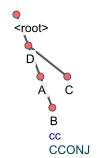
\includegraphics{img/nested1.png}
    \caption[Possible Wrong Attachments of a Coordinating Conjunction: Correct Conjunct as Wrong Head's Sibling]{Possible Wrong Attachments of a Coordinating Conjunction: Correct Conjunct as Wrong Head's Sibling.}
        Note: \textit{D} is the common ancestor of nodes \textit{A}, \textit{B} and \textit{C}\\
        Note: \textit{C} is the more relevant head that conjunction \textit{B} should be attached to, instead of the current misdirected attachment with node \textit{A}\\
        Note: \textit{A}, \textit{C} and \textit{D} might be the head of their own subtrees.
    \label{fig:conj-head1}
\end{figure}

\begin{figure}[H]
\begin{subfigure}{.45\textwidth}
  \centering
  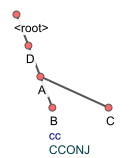
\includegraphics{img/nested2.png}
  \caption{Correct Conjunct as Conjunction's Sibling}
  \label{fig:conj-head2}
  \end{subfigure}
\begin{subfigure}{.5\textwidth}
  \centering
  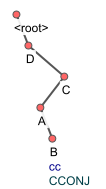
\includegraphics{img/nested3.png}
  \caption{Correct Conjunct as Conjunction's Grandparent}
  \label{fig:conj-head3}
\end{subfigure}
\caption[Possible Wrong Attachments of a Coordinating Conjunction]{Possible Wrong Attachments of a Coordinating Conjunction}
    Note: \textit{D} is the common ancestor of nodes \textit{A}, \textit{B} and \textit{C}\\
    Note: \textit{C} is the more relevant head that conjunction \textit{B} should be attached to, instead of the current misdirected attachment with node \textit{A}\\
    Note: \textit{A}, \textit{C} and \textit{D} might be the head of their own subtrees.
\label{fig:conj-head23}
\end{figure}

Notice that while the 3 cases as mentioned in Figures \ref{fig:conj-head1} and \ref{fig:conj-head23} are separate, there is no deterministic way of knowing what case an identified problematic instance might refer to. As such, we handle the 3 cases in decreasing order of priority, i.e. we try to handle the case as in Figure \ref{fig:conj-head1} first. In case the attempt fails, owing to multitude of reasons as explained later in Section \ref{ssec:conj_head_algorithm} (no siblings to attach to, lack of a candidate head in the siblings, for example), we try to solve it with respect to the case as in Figure \ref{fig:conj-head2}, and in case of a failure therein as well, eventually as in Figure \ref{fig:conj-head3}. If a particular instance is still not corrected after the consideration of the last case, we leave it unchanged.

\subsubsection{Conjunction Attached Non-Projectively}

In case of misdirected conjunctions that are attached non-projectively, the previous approach of limiting the level change with respect to the wrong head does not function well. The approach fails mainly because if the attachment is non-projective in nature, it is very likely that the conjunction is attached to a head in a different coordination. Consider the part of a sentence taken from UDv2.4 \verb|hi|-hdtb treebank in Example \ref{examp:conj_removed} and the tree for the corresponding example in Figure \ref{fig:conj_removed-wrong}. The token in bold is attached non-projectively because its current head is not a part of the same coordination structure as the conjunction itself.

\begin{example}
\label{examp:conj_removed}
\textbf{ }\\
\textbf{Text (\texttt{hi}):} \texthindi{वे सांसद \textbf{या} विधायक बनने के बाद लाभ के पद पर आसीन हैं या उससे पहले से हैं ।} \\
\textbf{Translit:} \textit{ve saamsad \textbf{yaa} vidhaayaka banane ke baada laabha ke pada para aasiin hain yaa usase pahale se hain .}\\
\textbf{Lit.:} they senator or legislator become-\textit{Inf.} \textit{Acc.} after power \textit{Poss.} position on situated are or therefrom before \textit{Dat.} are .\\
\textbf{Translated:} They have been in a position of power from before they became senator or legislator, or after.
\end{example}

\begin{figure}[H]
  \centering
  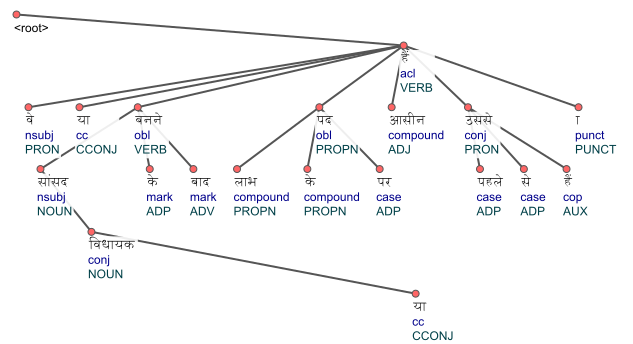
\includegraphics[scale=0.85]{img/removed-conj-wrong.png}
  \caption{Original Annotation for Example \ref{examp:conj_removed}}
  Note: First \texthindi{या} (\textit{yaa}, or) should be attached to \texthindi{विधायक} (\textit{vidhaayaka}; legislator), and not to \texthindi{हैं} (\textit{hain}; are)\\
  Note: Second \texthindi{या} (\textit{yaa}, or) should be attached to \texthindi{उससे} (\textit{usase}; therefrom), and not to \texthindi{विधायक} (\textit{vidhaayaka}; legislator)
  \label{fig:conj_removed-wrong}
\end{figure}

Since the conjunction is associated to a conjunct in the different coordination structure, the trivial approach to the problem is to look at the next available conjunct in the tree such that it satisfies the right-headedness criteria, and associate the conjunction to the said conjunct. In the previous example, the problem can simply be solved by associating the conjunction to the next available conjunct, marked by the deprel \verb|conj|. However, this might not be always possible if the next conjunct is not explicitly marked by the deprel. Consider the following example from UDv2.4 \verb|en|-EWT treebank and the associated dependency tree in Figure \ref{fig:nonconj}. The token of interest is marked in bold.

\begin{example}
\label{examp:nonconj}
\textbf{}\\
\textbf{But} other people do like the way they think he will vote, and the ones who favor him seem to outnumber the ones who oppose him .
\end{example}

\begin{figure}[H]
    \centering
    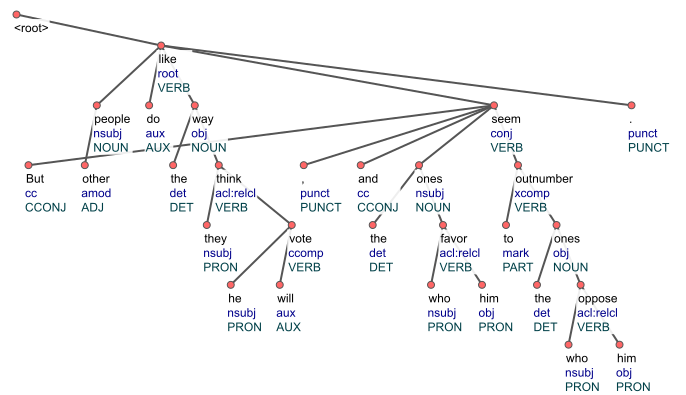
\includegraphics[scale=0.75]{img/nonconj.png}
    \caption{Dependency Tree for Example \ref{examp:nonconj}}
    Note: \textit{But} should be connected to \textit{like}, and not to \textit{seem}
    \label{fig:nonconj}
\end{figure}

In the example, the correct conjunct is not marked explicitly by the deprel \verb|conj|. Likewise in certain cases, the correct conjunct for the conjunction can not be found by the search for the deprel alone. However, based on the position of the content word token(s) that precede the conjunction in the word order, the correct conjunct can be determined to some extent. In the UDv2 guidelines, the dependencies that have a functional word as the head should be avoided (content-head dependency vs. function-head dependencies). Nonetheless, in some cases, the function words do form head of dependencies (when an auxiliary verb forms the root of a tree, for example). We treat the cases where the function word forms the head of a dependency as exceptional cases. As such, the correct conjunct position can be determined on the basis of the preceding content word token(s), including pronouns. The addition of pronouns is attributed to the fact that different pronouns can act as conjuncts in a sentence.

As can be seen in the last column in Tables \ref{tab:conjunctions_pud} and \ref{tab:conjunctions_all}, the misdirected dependencies such that they introduce non-projectivities are relatively uncommon. In our treatment of instances of the kind, we attempt to look for the next conjunct (if marked explicitly by the deprel) in the word order, such that the candidate conjunct follows the conjunction. In case the conjunct is not explicitly marked, we attempt to associate the conjunction to the immediately preceding content word in the word order. This ensures that the misdirection is not resolved, but the conjunction is now closer to the actual conjuncts and thus can be found in a process similar to the level-based analysis as done in previous subsection.

\subsection{Conjunction Sandwich}
\label{sec:conj-sand}

We have so far discussed only the cases where the problem can be identified by the wrong direction of dependency. However, when the direction of dependency is correct, mining for the problematic instances becomes troublesome. In Figure \ref{fig:conj_removed-wrong} reproduced below, notice that the first conjunction token \texthindi{या} (\textit{yaa}; or) is linked in the correct direction, but to the wrong head. This instance of the correct direction of attachment, albeit to wrong head can be present in the original annotation, or might be introduced after the tree has been corrected for the misdirected dependency. We refer to such cases as a Conjunction Sandwich, since the conjunction is sandwich-ed in between the conjuncts, with a wrong choice of head but with the direction of attachment being as expected (right-headed in our case). The problem of not being able to identify the correct conjunct as elaborated earlier in Example \ref{examp:nonconj} can manifest itself in such cases as well, making this problem significantly harder to detect.

\begin{reusefigure}[H]{fig:conj_removed-wrong}
    \centering
    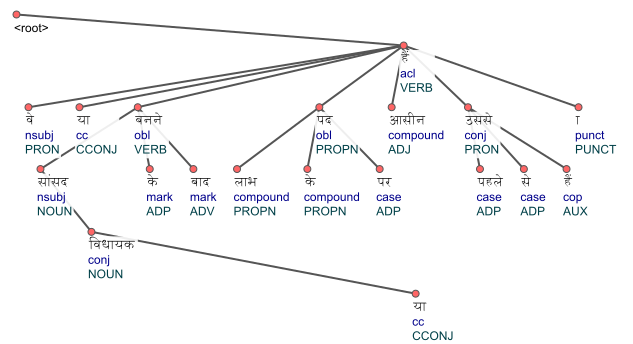
\includegraphics[scale=0.85]{img/removed-conj-wrong.png}
    \caption{Original Annotation for Example \ref{examp:conj_removed}}
    Note: First \texthindi{या} (\textit{yaa}; or) should be attached to \texthindi{विधायक} (\textit{vidhaayaka}; legislator), and not to \texthindi{हैं} (\textit{hain}; are)\\
  Note: Second \texthindi{या} (\textit{yaa}; or) should be attached to \texthindi{उससे} (\textit{usase}; therefrom), and not to \texthindi{विधायक} (\textit{vidhaayaka}; legislator)
\end{reusefigure}

In a given dependency tree, we can express node \(A\) being followed by node \(B\) in top-down ordering of tokens as \(A < B\). To establish node \(A\) is linked to node \(B\), such that \(A\) is the head of the relation, and \(B\) is the dependent, we can write \(A \rightarrow B\). In case where the direction of the relation is not important, we can express it by using double headed arrows as \(A \leftrightarrow B\). 

In a dependency tree, given two undirected edges \(i1 \leftrightarrow j1 \text{ and } i2 \leftrightarrow j2\), the edges are said to be overlapping if \(i1 < i2 < j1 < j2\) or \(i1 > i2 > j1 > j2\). In the example figure above, we can see that one of the ways in which a case of conjunction sandwich manifests itself is in the form of overlapping edges. However, this might not always be the case. The edges can overlap also because of the faulty annotation of other tokens in the tree, and that renders this check unreliable. In the example figure above, the edge containing the first conjunction also overlaps with the edge containing second conjunction, attached non-projectively. The constraint (of overlapping edges) was also tightened to look for a conjunction being the sole node in the gap of a non-projective attachment, but the number of cases that were flagged in the process remained very low (mostly less than 1\% of total number of conjunctions across different languages, depending on the language as some languages allow less number of non-projective structures than others). Of the total number of cases that were flagged by the tighter constraint, majority were false positives.

Consider the following example from UDv2.4 \verb|en|-lines treebank, and the associated dependency tree in Figure \ref{fig:unhandled-sandwich}. In this case, the edges do not overlap, but the conjunction is still attached to the wrong head.

\begin{example}
\label{examp:unhandled-sandwich}
\textbf{}\\
That was also mentioned by Mrs Oomen-Ruitjen \textbf{and} Mrs Glase.
\end{example}

\begin{figure}[H]
    \centering
    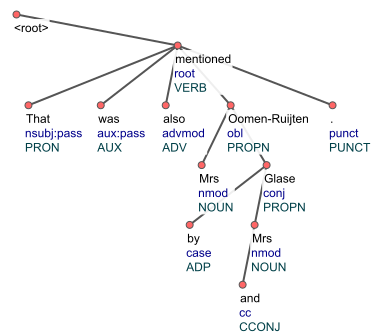
\includegraphics[scale=0.90]{img/unhandled-sandwich.png}
    \caption{Dependency Tree for Example \ref{examp:unhandled-sandwich}}
    Note: \textit{by} should be attached to \textit{Oomen-Ruitjen}, and not to \textit{Glase}\\
    Note: \textit{and} should be attached to \textit{Glase}, and not to \textit{Mrs}
    \label{fig:unhandled-sandwich}
\end{figure}

The trivial approach in the case of a Conjunction Sandwich would be to look for a conjunct explicitly marked by the \verb|conj| deprel, such that the said conjunct follows the conjunction in question. For example, in Figure \ref{fig:conj_removed-wrong}, the attachment for the first conjunction can be corrected by looking for the first explicitly marked conjunct that follows the current parent. This is an unreliable approach nonetheless, because (i) the conjunct needs to be explicitly marked by the deprel, which is not always the case; and (ii) the approach cannot work in the case of nested coordination, often picking up on a conjunct from another coordination structure.

Since none of the cases as discussed in this section could be reliably scouted for, we do not deal with identification and/or correction of Conjunction Sandwich in the current research.

\section{Dataset}
\label{ssec:conj_head_dataset}

The experiment was initially started on UDv2.3 \citep{UDv2.3}, but owing to the release of UDv2.4 \citep{UDv2.4} in May 2019, the experiment was transported entirely to UDv2.4. It is worth noting that there were far more cases of this problem being identified in UDv2.3, rather than in UDv2.4. Nonetheless, there exist significant cases of the problem (attachment of a conjunction to an incorrect head, and in wrong direction) in UDv2.4 as well.

We limit our treatment of the problem to \verb|af|, and \verb|ar|. As can be seen from Table \ref{tab:conjunctions_all}, the languages contain treebanks such that (i) they do not display any postposed variant of conjunctions as denoted by asterisk superscript in the table; (ii) the number of misdirected dependencies in the treebank is more than 10\% of the total number of conjunctions; and (iii) the languages do not have non-projectivity as a major characteristic, and yet the number of misdirected non-projective attachments is high in the treebank (unlike \verb|grc| and \verb|la| which have non-projectivity as a characteristic feature). Additionally, the languages belong to different language families viz. Germanic Indo-European and Semitic Afro-Asiatic, thus ensuring that the results of the experiment are not specific to a limited set of languages.

The number of instances of misdirected dependencies in different treebanks of UDv2.4 was highlighted in Table \ref{tab:conjunctions_pud} and \ref{tab:conjunctions_all}. The count of instances for \verb|af|\_afribooms and \verb|ar|\_padt are highlighted again in Table \ref{tab:dataset_conj} for reference.

\begin{table}[H]
    \centering
    \begin{tabular}{|l|l|l|l|l|}
        \hline
        \textbf{Treebank} & \textbf{Total} & \textbf{Misdirected} & \textbf{\% Total} & \textbf{Non-Proj}\\
        \hline
        \verb|af|\_afribooms & 1 832 & 1 829 & 99.836 & 130\\
        \verb|ar|\_padt & 13 855 & 1 411 & 10.184 & 80\\
        \hline
    \end{tabular}
    \caption{Misdirected Coordinating Conjunctions in UDv2.4 Treebanks for \texttt{af} and \texttt{ar}}
    \label{tab:dataset_conj}
\end{table}

\section{Experimental Setup}
\label{ssec:conj_head_experiment}

At the end of Section \ref{sec:conj-sand}, we mentioned how we would not deal with the cases where the direction of attachment is already correct. Thus, in the experiments, our treatment is limited to the instances with misdirected dependencies. To that resort, we start by identification of conjunctions such that they are associated in the wrong direction. Upon identification of such tokens, if they are attached non-projectively, we associate the token (still in the wrong direction) to the nearest content word that precedes the said token. In case the new attachment is now projective, we can terminate dealing with this case here. In the case of the new attachment being non-projective again, we try finding a content word (including pronouns) that is closest to the conjunction in word-order, and try attachment with this found word. If the new attachment is projective, we have dealt with the problem of non-projectivity for now, and the node in question can be associated to a more relevant head as other nodes that were originally projectively attached.

The problem with this approach (of reducing a case of non-projective attachment artificially to that of a projective attachment) is twofold. Primarily, the algorithm, as mentioned in Section \ref{ssec:conjunct-search}, looks for the candidate conjunct at a level that is determined by the attachment to the wrong conjunct. In principle, the choice of a wrong parent while solving non-projectivity could eventually lead to the corrected attachment with the wrong parent, resulting in a conjunction sandwich. Secondly, the approach does not take into account the cases when the attachment needs to be made to a function word, rather than a content word. The same issue can be raised for even the way the projective attachments are handled in general.

\section{Algorithm}
\label{ssec:conj_head_algorithm}

We start with defining some wrapper functions in Algorithm \ref{misdirected-edges-algo} and \ref{rollback-algo}. While the first one checks for the coordinating conjunctions that are attached in wrong direction, the second one tries to change the parent of the given node \(x\) to a new parent \(z\). In case the new attachment would be non-projective, the function rolls back to the previous parent. If projectivity is preserved, the function returns a \textbf{true} value, which allows us to terminate the function whenever the function call is made inside another function. The function also checks against making the node attached directly to the root of the tree, thereby making sure there is just one root node at any instance.

\begin{algorithm}[H]
\caption{misdirectedDependency()}
\label{misdirected-edges-algo}
    \begin{algorithmic}[1]
    \REQUIRE Node $x$
    \IF {$x.upos$ == ``CCONJ" \AND $x.udeprel$ == ``cc" \AND $x.parent.id$ < $x.id$}
        \RETURN \TRUE
    \ENDIF
    \RETURN \FALSE
    \end{algorithmic}
\end{algorithm}

\begin{algorithm}[H]
\caption{setParent()}
\label{rollback-algo}
    \begin{algorithmic}[1]
    \REQUIRE Node $x$, Original Parent $y$, New Parent Candidate $z$
    \STATE $x.parent \leftarrow z$
    \IF {$isnonprojective(x) == \TRUE$ \OR $z.id == 0$}
        \STATE $x.parent \leftarrow y$
        \RETURN \FALSE
    \ELSE
        \RETURN \TRUE
    \ENDIF
    \end{algorithmic}
\end{algorithm}

Having defined our wrapper functions, we start by trying to projectivize the conjunctions attached non-projectively in the wrong direction. We start by first looking for the next explicitly marked conjunct, and try to attach the conjunction to the said conjunct. We define this procedure in Algorithm \ref{algo:search-content}.

\begin{algorithm}[H]
\caption{nextConjHead()}
\label{algo:search-content}
    \begin{algorithmic}[1]
    \REQUIRE Node $x$ such that  $misdirectedDependency(x) == \TRUE$ \AND $isnonprojective(x) == \TRUE$, Original Parent $y$
    \STATE List $L \leftarrow$ containing nodes arranged in the increasing order of their $id$
    \STATE \COMMENT{i.e. $i < j \implies L[i].id < L[j].id \hspace{5mm} \forall L[i], L[j] \in L$}
    \FOR{node $z$ in $L$}
    \STATE \COMMENT{Process nodes in increasing order of their $id$}
        \IF {$z.id$ > $x.id$}
            \IF {$z.udeprel == ``conj"$}
                \RETURN $setParent(x, y, z)$
            \ENDIF
        \ENDIF
    \ENDFOR
    \RETURN \FALSE
    \end{algorithmic}
\end{algorithm}

In case of scenarios like in Example \ref{examp:conj_removed} (figure reproduced again below) with respect to the second conjunction, the non-projective attachment is made projective, and rectified with respect to the correct head automatically. However, there are cases when this approach may fail, owing to the next marked conjunct being located far away (and thus new attachment being non-projective again) or the next conjunct not being marked explicitly. In such cases, we move to the next step, and try to associate the current conjunction to the content word or pronoun that immediately precedes the given token. To look for the immediately preceding content word or pronoun, we look for the following POS tags- \verb|ADJ|, \verb|ADV|, \verb|NOUN|, \verb|PROPN|, \verb|VERB|, and \verb|PRON|. As with previous approach, we rollback the changes in case the attachment to new candidate head is non-projective in nature, going back to the original parent. The procedure is elaborated in Algorithm \ref{algo:conj-head-nonproj}.

\begin{reusefigure}[H]{fig:conj_removed-wrong}
    \centering
    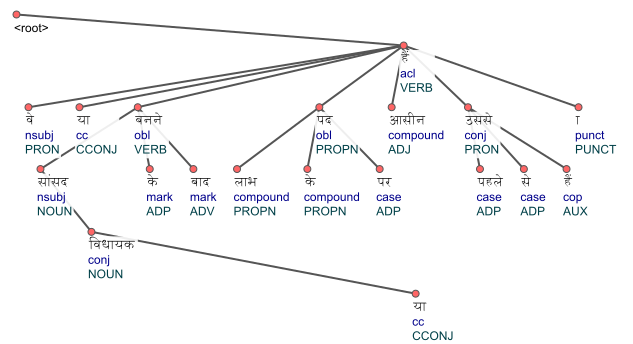
\includegraphics[scale=0.85]{img/removed-conj-wrong.png}
    \caption{Original Annotation for Example \ref{examp:conj_removed}}
    Note: First \texthindi{या} (\textit{yaa}; or) should be attached to \texthindi{विधायक} (\textit{vidhaayaka}; legislator), and not to \texthindi{हैं} (\textit{hain}; are)\\
  Note: Second \texthindi{या} (\textit{yaa}; or) should be attached to \texthindi{उससे} (\textit{usase}; therefrom), and not to \texthindi{विधायक} (\textit{vidhaayaka}; legislator)
\end{reusefigure}


\begin{algorithm}[H]
\caption{projTempFix()}
\label{algo:conj-head-nonproj}
\begin{algorithmic}[1]
\REQUIRE Node $x$ such that $misdirectedDependency(x) == \TRUE$ \AND $isnonprojective(x) == \TRUE$, Original Parent $y$
\STATE $candidates$ = []
\STATE \COMMENT{Empty List}
\FORALL{$z$ such that $z.id$ < $x.id$}
    \IF{$z.upos$ in $[``ADJ", ``ADV", ``NOUN", ``PROPN", ``VERB", ``PRON"]$}
        \STATE $candidates.append(z)$
        \STATE \COMMENT{Add $z$ to $candidates$ list}
    \ENDIF
\ENDFOR
\STATE \COMMENT{The content nodes are organised in the list, in word-order. We need to work with only the last candidate.}
\IF{$candidates$ == []}
    \RETURN \FALSE
\ELSE
    \STATE $candidate$ = $candidates[-1]$
    \STATE \COMMENT{Pick up the last element from $candidates$ list, and try changing it to head}
    \RETURN $setParent(x, y, candidate)$
\ENDIF
\end{algorithmic}
\end{algorithm}

Using the above algorithm, we are able to find better candidates for the originally misdirected non-projective dependency. Consider the following sentence, as taken from UDv2.4 \verb|af| treebank in Example \ref{examp:projTempFix}, and the corresponding original and modified annotations in Figure \ref{fig:projTempFixexample}, with the token of interest marked in bold. We can see that the original annotation contains the conjunction attached non-projectively. However, following the correction, the non-projectivity is solved and the new attachment is closer to the correct annotation. It is worth noting that the non-projectivity related to the punctuation marks can be solved easily (cf. Section \ref{ssec:punct-nonproj}).

\begin{example}
\label{examp:projTempFix}
\textbf{ }\\
\textbf{Text (\texttt{af}):} Ons onderwysteikens is eenvoudig , \textbf{maar} van kritiese belang.\\
\textbf{Lit:} Our educational-target\textit{-Pl.} is simple , \textbf{but} of critical significance .\\
\textbf{Translated:} Our educational targets are simple, but of critical significance.
\end{example}
\begin{figure}[H]
    \centering
    \begin{subfigure}{\textwidth}
    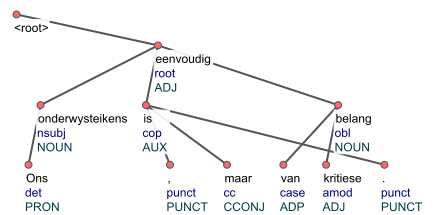
\includegraphics{img/projTempFixOriginal.png}
    \caption{Original Annotation}
    \end{subfigure}
    \begin{subfigure}{\textwidth}
    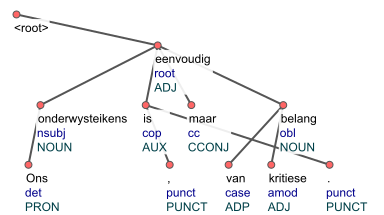
\includegraphics{img/projTempFixModified.png}
    \caption{Modified Annotation}  
    \end{subfigure}
    \caption{Change in Annotation for Example \ref{examp:projTempFix}}
    Note: \textbf{maar} (but) should be attached to \textbf{belang} (significance)
    \label{fig:projTempFixexample}
\end{figure}

At this point, we have exhausted our treatment of non-projective misdirected dependencies. A misdirected non-projective attachment of conjunction is either projective after this step, or is unaffected. We discuss the second case in Section \ref{ssec:conj_head-results} when we discuss the results of the experiment in more detail. For the first case of non-projective attachments, we have now removed the non-projectivity from the attachment, making sure they can be handled in the same manner as the other originally projective attachments, as elaborated earlier. 
% shown in Figures \ref{flow:conj_head_nonproj} and \ref{flow:conj_head_proj}.

For the common treatment of the attachments independent of their projectivity status, we look for the conjunctions such that they are attached in wrong direction. As a first step in search for a candidate conjunct, we look for the content words at the same level as the current node. We start by checking if there is a single remaining sibling that does not have a POS tag of \verb|X|, \verb|PUNCT|, or \verb|SYM| since we want to avoid the linking of the conjunction to these POS tags. In case of the condition being satisfied, and thus the availability of a single sibling as a candidate head, the token of interest is tried to be attached to this candidate head, and a \textbf{true} value is returned, indicating the success in search for the candidate. The effectiveness of case when a single sibling is present is demonstrated in Figure \ref{fig:singleSiblingAttach} containing an extension of the Example \ref{examp:projTempFix}, after the modification from Figure \ref{fig:projTempFixexample}.

\begin{figure}[H]
    \centering
    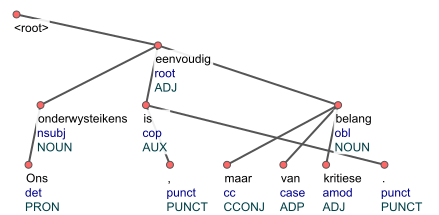
\includegraphics{img/projTempFixFinal}
    \caption{\textit{attachToSibling()}: Single Sibling Available}
    \label{fig:singleSiblingAttach}
\end{figure}

In case there are multiple siblings, we try to find the nearest sibling that has the deprel as \verb|conj|, and try attaching the conjunction to this marked conjunct. Essentially, this check would ensure that there is no need to search for another candidate, as the nearest sibling is the one that should be the head. In case the attachment to the marked conjunct will be non-projective in nature, the candidate would be located further away, and is not fit to being the head. However, this approach might fail owing to the conjunct not being explicitly marked. In the final search for the candidate conjunct in the siblings, we try to find the candidate by restricting the deprels to \verb|obl|, \verb|xcomp|, \verb|nmod|, and \verb|nsubj| amongst the siblings, attaching therein if such a case is found. 

The choice of the deprels is not arbitrary, but is based on an elimination procedure whereby we discarded most deprels. For selection of the candidate deprels, we restricted ourself to the core arguments, non-core dependents and nominal dependents that correspond to nominal and clausal structural categories\footnote{The first two columns, and the entries against the structural categories as indicated in \url{https://universaldependencies.org/u/dep/all.html}}. Of these relations, \verb|dislocated|, \verb|expl|, \verb|nummod|, \verb|vocative| can be outright discarded from the consideration. For \verb|appos|, the documentations marks explicitly the case where the deprel is chained in presence of a coordination\footnote{\url{https://universaldependencies.org/u/dep/appos.html}}, marking the subsequent tokens as \verb|conj|, rather than as \verb|appos|. The deprels \verb|acl| and \verb|advcl| function as clausal modifiers in form of an adjective\footnote{\url{https://universaldependencies.org/u/dep/acl.html}}, or an adverb\footnote{\url{https://universaldependencies.org/u/dep/advcl.html}} respectively. Since the dependents are explicitly clausal, we can very well discard them from consideration of conjuncts, alongwith \verb|appos|.

The documentations for the deprels \verb|obj|\footnote{\url{https://universaldependencies.org/u/dep/obj.html}} and \verb|iobj|\footnote{\url{https://universaldependencies.org/u/dep/iobj.html}} states that in presence of more than one proto-patients, the primary is to be labelled as \verb|obj|, and the rest as \verb|iobj|. However, even in presence of multiple objects (tri-transitive verbs are rare, but nonetheless present in Caucasian languages like Georgian, and Svan for example), the objects to the verb are often associated in form of causatives (cf. \cite[p.~39]{chirikba}, \cite[p.~43]{boeder}). This can be further extrapolated into a lack of conjunction between such objects of the tri-transitive verbs, thereby ensuring that we can safely discard the deprels \verb|obj| and \verb|iobj| from our consideration as well. 

The documentation\footnote{\url{https://universaldependencies.org/u/dep/csubj.html}} for deprel \texttt{csubj} states that the deprel is used when the subject itself is a clause. The guideline would ensure that there are very few cases when the deprels might be chained together by coordination, and even more so while they are at the same level in the tree. We therefore remove the deprel from consideration. 

Comparing the documentations of \texttt{ccomp}\footnote{\url{https://universaldependencies.org/u/dep/ccomp.html}} and \texttt{xcomp}\footnote{\url{https://universaldependencies.org/u/dep/xcomp.html}}, there is no way to say if either deprel is a better fit for the candidate head. In our experiments, the experiment performance went down when \texttt{ccomp} was included in the final list of head deprels. Keeping that in mind, we only include \texttt{xcomp} and discard \texttt{ccomp} from our consideration of candidate head deprels.

We could not find a strong reason for discarding the remaining deprels, viz. \verb|obl|, \verb|nmod|, and \verb|nsubj|, and thus included them with \verb|xcomp| in the list of deprels that can be searched for, while looking for a candidate conjunct.

The restriction with respect to deprels is necessary to make sure we don't over-generate and rehang the conjunction to a wrong head. In case the deprel is not restricted, the token of interest might associate itself to the wrong sibling, but in correct direction, making it as a case of conjunction sandwich (which as we mentioned earlier, is significantly harder to detect).

We formally define the constraints and the processing in Algorithm \ref{conj-head-sibling}. Notice how we decide on whether or not the algorithm terminates by continuously checking the condition of projectivity, and returning a value from the function only if the condition of projectivity with respect to the new parent is maintained. It is also important to note that we always limit our search for a suitable candidate to cases where the candidate occurs later than the conjunction we are trying to rehang.

\begin{algorithm}[H]
\caption{attachToSibling()}
\label{conj-head-sibling}
\begin{algorithmic}[1]
\REQUIRE $node$ such that $misdirectedDependency(node) == \TRUE$
\STATE \COMMENT{Try to attach to a sibling node}
\STATE $count \leftarrow 0$
\STATE $origParent \leftarrow node.parent$
    \FORALL {$siblings$ of $node$} \label{line:conj-sibling-countcheck1}
        \IF {$siblings.upos$ not in $[``X", ``PUNCT", ``SYM"]$ \AND $siblings.id > node.id$}
            \STATE $TargetSibling \leftarrow siblings$
            \STATE $count \leftarrow count + 1$
        \ENDIF
    \ENDFOR
    \IF {$count == 1$}
        \STATE \COMMENT{Just one sibling, attach to this sibling}
        \IF {$setParent(node, origParent, TargetSibling)$}
            \RETURN \TRUE
        \ENDIF
    \ENDIF \label{line:conj-sibling-countcheck2}
    \STATE \COMMENT{More than one siblings, narrow search by deprels}
    \FOR {$sibling$ of $node$}
        \IF {$sibling.udeprel == ``conj"$ \AND $sibling.id > node.id$}
            \IF {$setParent(node, origParent, sibling)$}
                \RETURN \TRUE
            \ENDIF
        \ENDIF
    \ENDFOR
    \FOR {$sibling$ of $node$}
        \IF {$sibling.udeprel$ in $[``obl", ``xcomp", ``nmod", ``nsubj"]$ \AND $node.id < sibling.id$}
            \IF {$setParent(node, origParent, sibling)$}
                \RETURN \TRUE
            \ENDIF
        \ENDIF
    \ENDFOR
\RETURN \FALSE
\end{algorithmic}
\end{algorithm}

If there is no suitable candidate in the same level as the current level of the conjunction, we try to ascend one level and try to attach the node to the next aunt (parent's sibling) in Algorithm \ref{conj-head-aunt}. The condition may arise owing to not finding a suitable candidate in siblings, or in case where there are no siblings to search for. We do not set any checks with respect to deprels, but still keep a check on the condition of projectivity and the node order. Consider the following part of sentence from \verb|af| treebank in Example \ref{examp:auntAttach} with the corresponding annotations in Figure \ref{fig:auntAttach}, with the token of interest marked in bold. Figure \ref{fig:auntAttach-2} shows the part where the algorithm connects the conjunction to the parent's sibling, after having failed trying to find an attachment amongst the siblings.

\begin{algorithm}[H]
\caption{attachToAunt()}
\label{conj-head-aunt}
\begin{algorithmic}[1]
\REQUIRE $node$ such that $misdirectedDependency(node) == \TRUE$
\STATE \COMMENT{Try to attach to the first relevant aunt node}
\STATE $origParent \leftarrow node.parent$
\STATE $aunts = []$
\FOR {$sibling$ of $origParent$}
    \IF {$sibling.id > node.id$}
        \STATE $aunts$.append($sibling$)
    \ENDIF
\ENDFOR
\STATE \COMMENT{The candidate aunts would be arranged in word-order in the $aunts$ list}
\IF {$aunts$ is not empty}
    \STATE $setParent(node, origParent, aunts[0])$
\ENDIF
\RETURN \FALSE
\end{algorithmic}
\end{algorithm}

\begin{example}
\label{examp:auntAttach}
\textbf{ }\\
\textbf{Text (\texttt{af}):} Indien die laaste dag vir betaling op 'n openbare vakansiedag \textbf{of} oor die naweek val, ... \\
\textbf{Lit:} In-the-event-that the last day for pay on a public holiday \textbf{or} over the weekend fall, ...\\
\textbf{Translated:} If the last day for payment falls on a public holiday or over the weekend, ...
\end{example}

\begin{figure}
    \centering
    \begin{subfigure}{\textwidth}
    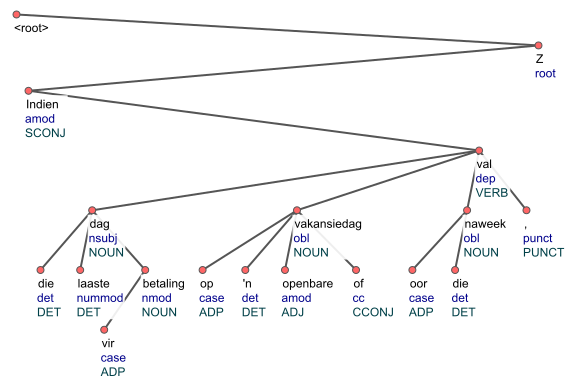
\includegraphics[scale=0.80]{img/auntAttachOriginal.png}
    \caption{Original Annotation}
    \label{fig:auntAttach-1}
    \end{subfigure}
    \begin{subfigure}{\textwidth}
    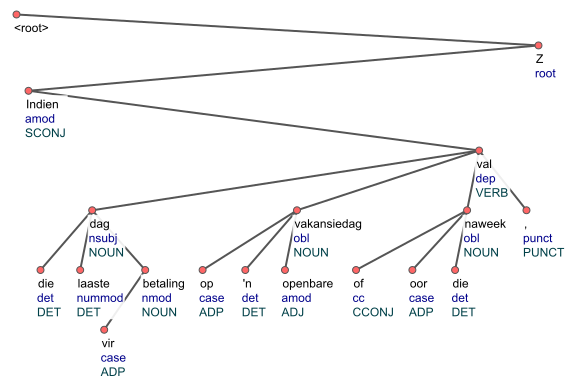
\includegraphics[scale=0.80]{img/auntAttachFinal.png}
    \caption{Modified Annotation after attachToAunt()}
    \label{fig:auntAttach-2}
    \end{subfigure}
    \caption{Change in Annotation for Example \ref{examp:auntAttach}}
    Note: \textit{Z} is used to denote the position of original root of the sentence\\
    Note: \textbf{of} (or) should be attached to \textbf{naweek} (weekend)
    \label{fig:auntAttach}
\end{figure}

In the event that a suitable candidate is not found, a \textbf{false} value is returned. This implies that our search for a suitable candidate has failed even after trying to ascend one level. As last resort, we try to attach the conjunction to the grandparent, while preserving projectivity in Algorithm \ref{conj-head-granny}. An example of case where this function is needed is elaborated in Example \ref{examp:granny} containing the sentence from \verb|af| treebank, with the corresponding annotations in Figure \ref{fig:granny}.

\begin{algorithm}[H]
\caption{attachToGrandparent()}
\label{conj-head-granny}
\begin{algorithmic}[1]
\REQUIRE $node$ such that $misdirectedDependency(node) == \TRUE$
\STATE \COMMENT{Try to attach to the grandparent node}
\STATE $origParent \leftarrow node.parent$
\STATE $grandparent \leftarrow origParent.parent$
\IF {$setParent(node, origParent, grandparent)$}
    \RETURN \TRUE
\ENDIF
\RETURN \FALSE
\end{algorithmic}
\end{algorithm}

\begin{example}
\label{examp:granny}
\textbf{ }\\
\textbf{Text (\texttt{af}):} Ons onderwys- \textbf{en} vaardigheidsprogramme sal ons produktiwiteit en mededingendheid verhoog . \\
\textbf{Lit:} Our education- \textbf{and} skills-program-\textit{Pl.} shall our productivity and competitiveness increase .\\
\textbf{Translated:} Our education and skills programs will increase our productivity and competitiveness.
\end{example}

\begin{figure}[H]
    \centering
    \begin{subfigure}{\textwidth}
    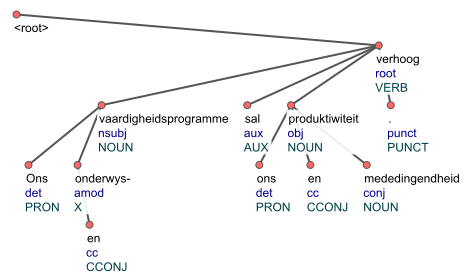
\includegraphics[scale=0.80]{img/grannyOriginal.png}
    \caption{Original Annotation}
    \label{fig:granny-1}
    \end{subfigure}
    \begin{subfigure}{\textwidth}
    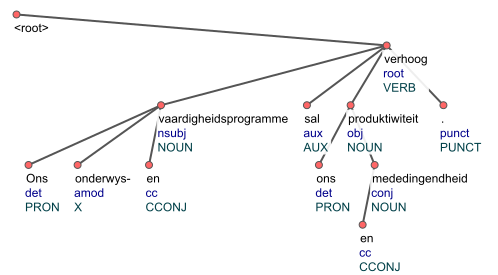
\includegraphics[scale=0.80]{img/grannyModified.png}
    \caption{Modified Annotation after attachToGrandparent()}
    \label{fig:granny-2}
    \end{subfigure}
    \caption{Change in Annotation for Example \ref{examp:granny}}
    Note: \textbf{en} (and) should be attached to \textbf{vaardigheidsprogramme} (skills-program)
    \label{fig:granny}
\end{figure}

Having established all the possible cases, we can wrap them all in a nice function that takes care of all the cases, in priority order. Algorithm \ref{conj-head-algo} shows the complete algorithm, in order of execution of the functions defined throughout the section.

\begin{algorithm}[H]
\caption{fixconjhead()}
\label{conj-head-algo}
\begin{algorithmic}[1]
\REQUIRE $node$ such that $misdirectedDependency(node) == \TRUE$
\IF{$isnonprojective(node)$ == \TRUE}
    \IF{\NOT{$nextConjHead(node, node.parent)$}}
        \IF{\NOT{$projTempFix(node, node.parent)$}}
            \STATE Do Nothing
        \ENDIF
    \ENDIF
\ENDIF
\STATE \COMMENT{Made non-projective attachments projective}
\IF {$attachToSibling(node)$}
    \RETURN 
\ELSIF{$attachToAunt(node)$}
    \RETURN
\ELSIF{$attachToGrandparent(node)$}
    \RETURN
\ELSE
    \RETURN
\ENDIF
\end{algorithmic}
\end{algorithm}

\section{Results and Evaluation}
\label{ssec:conj_head-results}

We implement the algorithm in form of a Udapi-python \citep{udapi} block\footnote{Code alongwith manually annotated data available at \url{https://github.com/Akshayanti/Masters-Thesis-CUNI-2020/tree/master/conj_head}}. The runtime of the block for the data is as mentioned in Table \ref{tab:conj-head-runtime}, as run on Ubuntu 18.04 (64-bit) on a 4-core Intel i5-6300 HQ processor.

\begin{table}[H]
    \centering
    \begin{tabular}{|l|l|}
        \hline
        \textbf{Language} & \textbf{Time (in ms)}\\
        \hline
        \verb|af| & \(81.33 \pm 7.094\) \\
        \verb|ar| & \(317.05 \pm 23.996\) \\
        \hline
    \end{tabular}
    \caption{Average Runtime (\(\pm\) sd) for Udapy Python Block Implementation}
    Note: Does Not include time taken to read the original CoNLL-U file
    \label{tab:conj-head-runtime}
\end{table}

In this section, we would first evaluate the treatment of originally nonprojective attachments with respect to the individual segments of the algorithm, followed by a discussion of the instances not handled by the algorithm dealing specifically with nonprojective attachments. The instances were manually annotated for the direction of dependency, as well as for the choice of the correct head. Next, we would look at the part of the algorithm that is common to all tokens, irrespective of their projectivity status. Our focus would be on the nodes that were affected at major steps, and the nodes that were unaffected by the end of the algorithm. We then look at the overall evaluation of the algorithm, as manually annotated for the correct attachment to the parent node, on limited subsamples.

\subsection{Originally Non-Projective Attachments}

The number of originally nonprojective nodes affected by the first part of the algorithm, where they were associated with either the next marked conjunct, or where their attachment was temporarily made projective is as listed in Table \ref{tab:affectedNodes1}. We discuss on the effect of individual functions in the following subsections.

\begin{table}[H]
\centering
    \begin{tabular}{|l|l|l|l|l|}
        \hline
        \textbf{Lang.} & \textbf{Total} & \textit{nextConjHead()} & \textit{projTempFix()} & Unaffected\\
        \hline
        \texttt{af} & 130 & 20 & 106 & 5\\
        \texttt{ar} & 80 & - & 44 & 36\\
        \hline
    \end{tabular}
    \caption{Nodes Affected: Non Projective Attachment}
    \label{tab:affectedNodes1}
\end{table}

\subsubsection{Effect of \textit{nextConjHead()}}

Of all the nodes affected by \textit{nextConjHead()} algorithm (cf. Algorithm \ref{algo:search-content}), 85\% of the nodes were associated to the right parent. Of the remaining 15\%, we found annotation errors which resulted in a failure in identification of the more relevant head. The annotation errors in these case were primarily associated with the wrong token being marked as a conjunct, or an explicitly marked conjunct of another coordination structure being selected as candidate (the conjunct in current coordination structure was not explicitly marked). While the modified annotation in these cases corrected the direction of dependency, there was a failure in determination of the correct head of attachment. This is a case of conjunction sandwich, as discussed earlier, and introduced in this context owing to a faulty correction. An example of such case is shown in Example \ref{examp:nextConjHead-wrong}, with the associated annotations in Figure \ref{fig:nextConjHead-wrong}. As before, the token of interest is marked in bold.

\begin{example}
\label{examp:nextConjHead-wrong}
\textbf{ }\\
\textbf{Text (\texttt{af}):} ... in hulle huise, op straat \textbf{en} op die pad in voortdurende angs verkeer ...\\
\textbf{Lit:} ... in \textit{3Pl-Poss.} house, on street \textbf{and} on the path-\textit{Sg.} in continuous anxiety find-\textit{Pres.} ...\\
\textbf{Translated:} ... in their house, on street and on the road in continuous anxiety ...
\end{example}

\begin{figure}[H]
    \begin{subfigure}{.49\textwidth}
     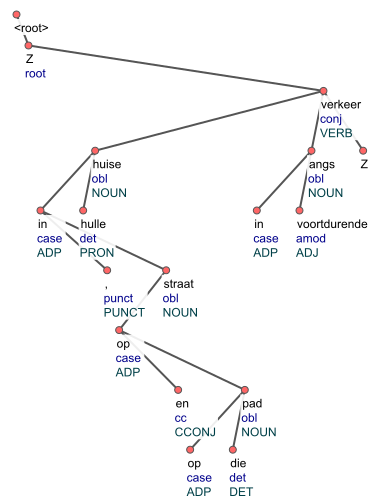
\includegraphics[scale=0.69]{img/nextConjHead-wrong1.png}
     \caption{Original Annotation}
    \end{subfigure}
    \begin{subfigure}{.5\textwidth}
    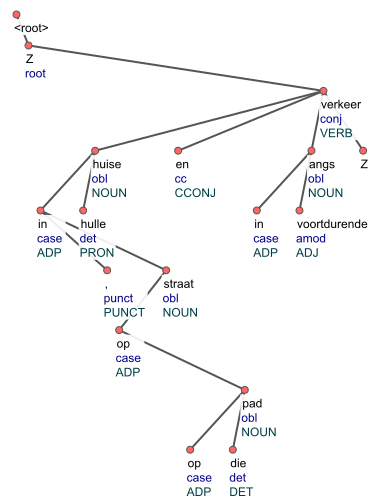
\includegraphics[scale=0.69]{img/nextConjHead-wrong2.png}
     \caption{Final Annotation}
    \end{subfigure}
    \caption{Annotation Error in Example \ref{examp:nextConjHead-wrong}}
    Note: Z is used as a placeholder for ellipsed text\\
    Note: \textbf{,} should be attached to \textbf{huise} (house) or to the immediately succeeding \textbf{op} (on)\\
    Note: \textbf{straat} (street) and its children should be attached to \textbf{verkeer} (find-\textit{Pres.})\\
    Note: \textbf{en} (and) should be attached to \textbf{pad} (path-\textit{Sg.}) \\
    Note: \textbf{pad} (path-\textit{Sg.}) and its children should be attached to \textbf{verkeer} (find-\textit{Pres.})\\
    Note: \textbf{verkeer} (find-\textit{Pres.}) is wrongly marked as \verb|conj|
    \label{fig:nextConjHead-wrong}
\end{figure}

\subsubsection{Effect of \textit{projTempFix()}}

Table \ref{tab:projTempFixResults} shows the number of instances that were forced into a projective attachment when \textit{projTempFix()} algorithm (cf. Algorithm \ref{algo:conj-head-nonproj}) was used on them. The total count of such instances is listed in the second column. The values in third column onward refer to the results of the manual verification, verified with respect to the direction of new attachment and the relevancy of the choice of head for the new attachment. The manual verification was done after the projectivised token was subjected to the overall algorithm. The third column refers specifically to the cases where the direction was corrected, but the choice of head of attachment was not correct, thereby resulting in a conjunction sandwich. The value in the fourth column refers to the count of tokens that had no change whatsoever in their attachment, before and after the algorithm. The value in the last column represents the count of tokens such that the attachment to new parent was correct in both the aspects.

\begin{table}[H]
    \centering
    \begin{tabular}{|l|l|l|l|l|}
    \hline
    \textbf{Lang.} & \textbf{Total} & Conj. Sand. & Unfixed & Correct\\
    \hline
    \texttt{af} & 106 & 12 & 91 & 3\\
    \texttt{ar} & 44 & - & 42 & 2\\
    \hline
    \end{tabular}
    \caption{Evaluation: \textit{projTempFix()}}
    \label{tab:projTempFixResults}
\end{table}

While the results for the forced projectivisation are primarily negative, there seems to be a pattern to the results. In the analysis of the instances marked as unfixed for either language, it was found that the correct attachment was not possible because the relevant part of the dependency tree had the original annotation wrong and non-projective while the correct annotation would be projective. Consider one such instance in Example \ref{examp:projTemp00}, and the associated dependency trees in Figure \ref{fig:projTemp00}, with the token of interest marked in bold. Notice the adposition \textbf{van} (of) being shared wrongly with \textbf{kultuur} (culture) token in Figures \ref{projTempFix00-orig}, \ref{projTempFix00-mod}. The overall corrected annotation is reflected in Figure \ref{projTempFix00-correct1}.

\begin{example}
\label{examp:projTemp00}
\textbf{ }\\
\textbf{Text (\texttt{af}):} ``deure van geleerdheid \textbf{en} van kultuur"\\
\textbf{Lit:} `` doors of learning \textbf{and} of culture " \\
\textbf{Translated:} ``doors of learning and of culture"
\end{example}

\begin{figure}[H]
    \begin{subfigure}{.45\textwidth}
    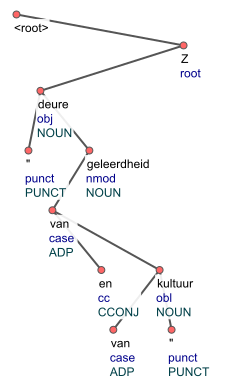
\includegraphics[scale=0.80]{img/projTempFix00-orig.png}
    \caption{Original Annotation}
    \label{projTempFix00-orig}  
    \end{subfigure}
    \begin{subfigure}{.5\textwidth}
    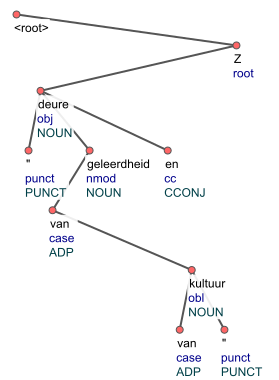
\includegraphics[scale=0.80]{img/projTempFix00-mod.png}
    \caption{Final Annotation}
    \label{projTempFix00-mod}  
    \end{subfigure}
    \begin{subfigure}{\textwidth}
    \centering
    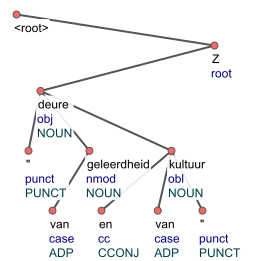
\includegraphics[scale=0.80]{img/projTempFix00-correct1.png}
    \caption{Overall Corrected Annotation}
    \label{projTempFix00-correct1}  
    \end{subfigure}
    \caption{Dependency Trees for Example \ref{examp:projTemp00}}
    Note: \textit{Z} is used to denote the node where the subtree is attached in the original sentence
    \label{fig:projTemp00}
\end{figure}

The problem of the false annotations with respect to non-projectivity is an open problem that is not handled in the current work. The problem is discussed in brief in Section \ref{future:nonproj}. In the current context, the cases of conjunction sandwich are also attributed to such wrong annotations. Consider the sentence from \verb|af| treebank in Example \ref{examp:projTemp01} and the associated dependency trees in Figure \ref{fig:projTemp01}, with the token of interest marked in bold. Note that the adposition \textbf{vir} (for) is shared wrongly by \textbf{besending} (consignment), bringing false non-projectivity into the sentence structure. 

\begin{example}
\label{examp:projTemp01}
\textbf{ }\\
\textbf{Text (\texttt{af}):} Hierdie permit is vir 'n beperkte tydperk \textbf{en} vir slegs een besending geldig .\\
\textbf{Lit:} this permit is for a limited period \textbf{and} for only one consignment valid . \\
\textbf{Translated:} This permit is valid for a limited period and for only one consignment.
\end{example}

\begin{figure}[H]
    \begin{subfigure}{\textwidth}
    \centering
    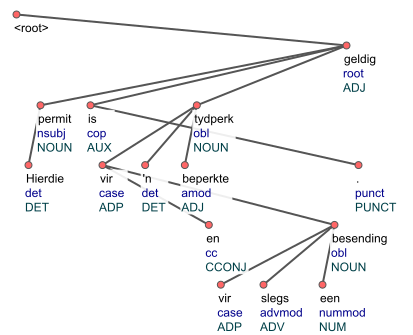
\includegraphics[scale=0.80]{img/projTempFix01-orig.png}
    \caption{Original Annotation}
    \label{projTempFix01-orig}  
    \end{subfigure}
    \begin{subfigure}{\textwidth}
    \centering
    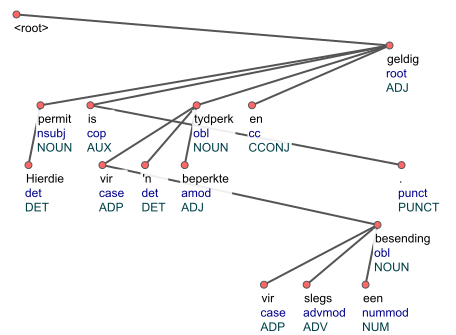
\includegraphics[scale=0.80]{img/projTempFix01-mod.png}
    \caption{Final Annotation}
    \label{projTempFix01-mod}  
    \end{subfigure}
    \caption{Dependency Trees for Example \ref{examp:projTemp01}}
    Note: \textbf{besending} (consignment) should be linked to \textbf{geldig} (valid)\\
    Note: \textbf{en} (and) should be linked to \textbf{besending} (consignment)\\
    Note: \textbf{.} should be linked to \textbf{geldig} (valid)
    \label{fig:projTemp01}
\end{figure}


\subsubsection{Non-Projective Attachments Not Handled}

All the cases that were unprocessed after the attempt at projectivisation of non-projective attachments were processed by the overall algorithm. We do not discuss here the statistics on the correction procedure of such cases, but leave it for the next section when we evaluate the overall algorithm. 

\subsection{Processing Pipeline Independent of Projectivity of Attachment}

As can be seen from Table \ref{tab:affectedNodesOverall}, the manual evaluation if done on a randomly chosen sample of the affected nodes would be very heavily biased on the results from \textit{attachToSibling()} algorithm. To counter this effect, we decided to separately evaluate the algorithms, and so a random sample of 100 affected nodes was chosen containing the nodes affected by \textit{attachToSibling()} algorithm only. To measure the efficiency of \textit{attachToAunt()} and \textit{attachToGrandparent()} algorithms, another sample containing upto 100 randomly sampled instances was chosen. All the sampled instances were then manually annotated for the correctness in their attachment to the correct conjunct, as well as the direction of the attachment.

\begin{table}[H]
    \centering
    \scalebox{0.8}{
    \begin{tabular}{|l|l|l|l|l|l|}
        \hline
        \textbf{Lang.} & \textbf{Total} & \textit{attachToSibling()} & \textit{attachToAunt()} & \textit{attachToGrandparent()} & Unaffected\\
        \hline
        \texttt{af} & 1809 & 1665 & 8 & 124 & 12 \\
        \texttt{ar} & 1411 & 952 & 58 & 178 & 223 \\
        \hline
    \end{tabular}}
    \caption{Nodes Affected: Overall}
    \label{tab:affectedNodesOverall}
\end{table}

\subsubsection{Overall Evaluation}

We estimated the effect of \textit{projTempFix()} earlier, and so to estimate the effects of the different algorithms in an overall manner, such tokens were not included in either sample. Furthermore, the difference between the total count of instances and the listed instances identified as either of correct or as a case of conjunction sandwich marks the number of instances that were still misdirected in their attachment. Table \ref{tab:evalOverall} lists the results of the manual evaluation.

\begin{table}[H]
    \centering
    \begin{tabular}{|l|l|l|l|l|l|l|}
    \hline
    \multicolumn{1}{|l|}{\textbf{Algo.} \(\rightarrow\)} &
    \multicolumn{3}{c|}{\textit{attachToSibling()}} &
    \multicolumn{3}{c|}{Others}\\
    \textbf{Lang. \(\downarrow\)} & \textbf{Total} & Conj. Sand. & Correct & \textbf{Total} & Conj. Sand. & Correct\\
    \hline
    \texttt{af} & 100 & 1 & 99 & 32 & 1 & 22\\
    \texttt{ar} & 100 & 2 & 98 & 100 & 4 & 28\\
    \hline
    \end{tabular}
    \caption{Overall Evaluation of Affected Nodes on Randomly Sampled Instances}
    \label{tab:evalOverall}
\end{table}

We based \textit{attachToSibling()} algorithm based on the assumption that we would not need to descend the tree level in the search for the correct conjunct and that we need to only ascend the level in the tree. In the analysis of instances with an introduced conjunction sandwich in \verb|ar|, the correct conjunct could have been found by descending the tree level. Example \ref{examp:siblingAttachar} shows the relevant part of one such example, with the corresponding dependency trees before and after the correction procedure in Figures \ref{fig:siblingAttach-ar-1} and \ref{fig:siblingAttach-ar-2} respectively. In the example, \textit{Z} is used to denote the ellipsed part of the tree, while \textit{Root} is used to donate the root of the tree. The token of interest is marked in bold.

\begin{example}
\label{examp:siblingAttachar}
\textbf{ }\\
\textbf{Text (\texttt{ar} in RTL):} ... Z \textarabic{
\textbf{ف}مع  انتهاء   ما بدا فصلاً من معركتها مع المعارضة ، بات }
. Z ...\\
\textbf{Translit (Top-down):} Z . \textbf{f}-mae aintiha' ma bada fslaan min maerakat-ha mae almuearadat , bat Z\\
\textbf{Lit. (Top-down):} ... . \textbf{And}-with finishing what appear-\textit{Perf.}-\textit{3P.} chapter from battle-it-\textit{3P.}-\textit{Sing.} with opposition , become-\textit{Perf.}-\textit{3P.} Z\\
\textbf{Translated:} ... . With the end of what appeared to be a chapter in the battle against the opposition, it became ...  
\end{example}

\begin{figure}[H]
    \begin{subfigure}{\textwidth}
    \centering
    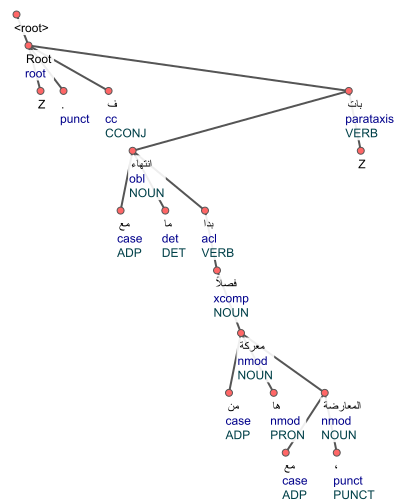
\includegraphics[scale=0.7]{img/siblingAttach-ar-1.png}
    \caption{Original Annotation}
    \label{fig:siblingAttach-ar-1}
    \end{subfigure}
    \newline
    \begin{subfigure}{\textwidth}
    \centering
    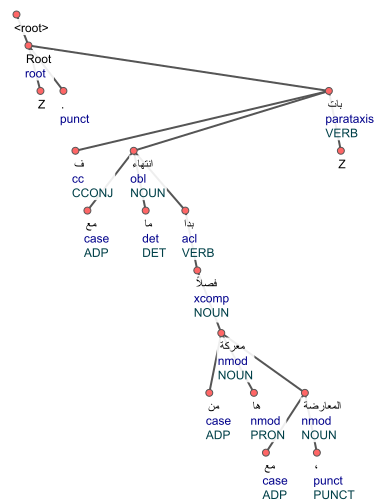
\includegraphics[scale=0.7]{img/siblingAttach-ar-2.png}
    \caption{Final Annotation}
    \label{fig:siblingAttach-ar-2}
    \end{subfigure}
    \caption{Introduced Conjunction Sandwich in \texttt{ar}}
    Note: Z is used as a placeholder for ellipsed text\\
    Note: Root is used as a placeholder for root of the tree\\
    Note: \textarabic{ف} (\textit{f}; And) should be attached to \textarabic{انتهاء} (\textit{aintiha'}; finishing) and not to \textarabic{بات} (\textit{bat}; become-\textit{Perf.}-\textit{3P})
    \label{fig:siblingAttach-ar}
\end{figure}

 In case of \verb|af|, the actual conjunct could not be discovered because of the improper annotation of the subtree. The modification as done by \textit{attachToSibling()} algorithm attached the conjunction to where the conjunct should have been. Attachment to the right conjunct in this case was not possible because (i) the change of levels in present annotation would bypass the enforced limit of one level; and (ii) the new attachment would have been non-projective in nature, and was therefore not allowed. Example \ref{examp:siblingAttachaf} and the associated dependency trees in Figure \ref{fig:siblingAttach-af} demonstrate this with a part of the actual sentence. As in previous example, \textit{Z} is used to denote the ellipsed part of the tree, while also showcasing the relative position of the root of the tree. The token of interest is marked in bold.
 
\begin{example}
\label{examp:siblingAttachaf}
\textbf{ }\\
\textbf{Text (\texttt{af}):} Deur bewusmakingsveldtogte \textbf{en} inderdaad as gevolg van die vennootskappe Z\\
\textbf{Lit:} Through awareness-campaigns \textbf{and} indeed as consequence of the partnerships ...\\ 
\textbf{Translated:} Through awareness campaigns \textbf{and} indeed because of the partnerships ...
\end{example}

\begin{figure}[H]
    \begin{subfigure}{.48\textwidth}
    \centering
    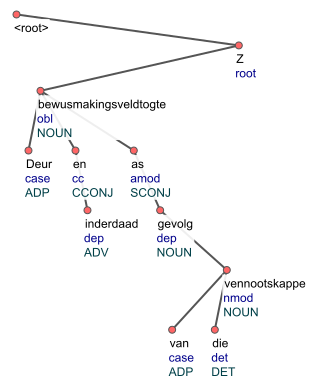
\includegraphics[scale=0.8]{img/siblingAttach-af-1.png}
    \caption{Original Annotation}
    \label{fig:siblingAttach-af-1}
    \end{subfigure}
    % \newline
    \begin{subfigure}{.5\textwidth}
    \centering
    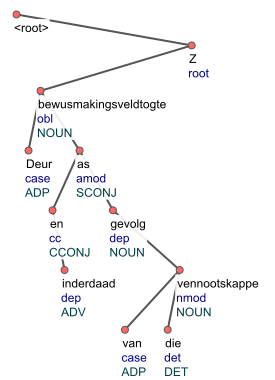
\includegraphics[scale=0.8]{img/siblingAttach-af-2.png}
    \caption{Final Annotation}
    \label{fig:siblingAttach-af-2}
    \end{subfigure}
    \caption{Introduced Conjunction Sandwich in \texttt{af}}
    \label{fig:siblingAttach-af}
    Note: Z is used as a placeholder for ellipsed text, and also to mark the position of the root of the tree\\
    Note: \textbf{gevolg} (consequence) should be the head of the subtree, with \textbf{as} (as) attached to it\\
    Note: \textbf{inderdaad} (indeed) should be attached to \textbf{gevolg} (consequence) after the change of subtree head\\
    Note: \textbf{en} (and) should be attached to \textbf{gevolg} (consequence) after the change of subtree head
\end{figure}

The instances of misdirected dependency in conjunctions that escaped processing by \textit{attachToSibling()} algorithm were then processed by algorithms \textit{attachToAunt()} and \textit{attachToGrandparent()} in that order. We found that the majority of these cases were still misdirected even after being processed by the overall algorithm. We discuss such cases in the next section where we discuss some insights into the processing of the algorithm step by step. Of the instances that led to a case of conjunction sandwich, the majority of the cases were caused by an annotation error, caused due to improper selection of the head of the relevant subtree. The example from \verb|af| treebank in Example \ref{examp:others-conj-sand}, and the associated dependency tree in Figure \ref{fig:others-conj-sand} demonstrates this. In the example, the conjunction sandwich is caused because of the improper annotation in the tree. The conjunction of interest is marked in bold.

\begin{example}
\label{examp:others-conj-sand}
\textbf{ }\\
\textbf{Text (\texttt{af}):} Die derde taal kan 'n amptelike \textbf{of} 'n vreemde taal wees.\\
\textbf{Lit:} The third language can a official \textbf{or} a alien language be .\\ 
\textbf{Translated:} The third language may be an official or a foreign language .
\end{example}

\begin{figure}[H]
    \begin{subfigure}{\textwidth}
    \centering
    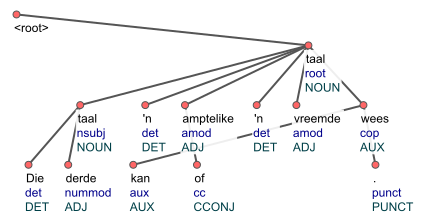
\includegraphics[scale=0.90]{img/others-conj-sand-1.png}
    \caption{Original Annotation}
    \label{fig:others-conj-sand-1}
    \end{subfigure}
    \begin{subfigure}{\textwidth}
    \centering
    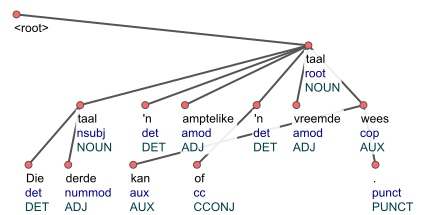
\includegraphics[scale=0.90]{img/others-conj-sand-2.png}
    \caption{Modified Annotation}
    \label{fig:others-conj-sand-2}
    \end{subfigure}
    \caption{Change in Annotation for Example \ref{examp:others-conj-sand}}
    Note: \textbf{of} (and) should be attached to \textbf{vreemde} (alien) and not to \textbf{'n} (a)\\
    \label{fig:others-conj-sand}
\end{figure}

\subsubsection{Unaffected Nodes}

By unaffected nodes, we refer to the instances of misdirected dependency which were not at all touched by the entire algorithm. We hypothesized earlier that if the rehanging of the node requires a change in more than one level (of the level of wrong conjunct), it is likely to be an annotation error that needs manual correction. We found that to be true for more than 50\% of the cases in either treebank with respect to all the unaffected cases. For the remaining cases, the major reason why the node could not be rehung was associated with the limit of deprels in \textit{attachToSibling()} algorithm. Since that was also the case for a majority of cases where the misdirected dependency persisted, we discuss the unaffected nodes with them in the final discussion.

\section{Discussion and Conclusion}

We started trying to handle the cases of conjunctions that were attached non-projectively to the parent, and employed algorithms \textit{nextConjHead()} and \textit{projTempFix()} to find a better candidate. We got mixed results for the nodes. From our understanding of the patterns exhibited in the two languages, the first algorithm works only if there exists an explicitly marked conjunct. This was true in case of \verb|af| where the conjuncts are explicitly marked with \verb|conj| deprel, but when the conjuncts are not explicitly marked (as in case of \verb|ar|), the algorithm doesn't work as intended. 

The force projectivisation in \textit{projTempFix()} algorithm didn't work as expected. In the analysis of the instances, we found that this was mainly due to falsely annotated non-projectivities. In general, if the conjunction was in gap of another non-projective attachment to the same parent, the algorithm didn't work. The inefficiency of the algorithm in such cases could be exhibited in the form of node not being affected at all, or the new attachment eventually leading to a case of conjunction sandwich. If the conjunction (and any punctuation nodes attached to this token) is the only non-projective attachment to the parent, the algorithm would be able to make the correction effectively, and without an error.

Given the aforementioned concerns about the algorithms, it would be recommended to not use the algorithms in case of a language that displays high amount of non-projectivity in sentence structures (for example, \verb|grc|) and/or on a treebank has not been checked for the annotation consistency of the non-projective structures (as in the scope of the current experiment). Furthermore, in a case where the algorithms are used, it would be advised to have an annotator look at the corrections for higher reliability.

The common part of the pipeline started with \textit{attachToSibling()} algorithm that seeks to associate a misdirected conjunction to a sibling token, attached to the same parent. The number of cases that were found to introduce a case of conjunction sandwich could have been caused due to multiple reasons. We limited the search of a candidate head by the candidate's UPOS (more specifically, blacklisting a few UPOS) in case of a single available candidate, as mentioned earlier in the definition of the algorithm. In the event of the candidate being marked by the blacklisted UPOS, no matter the choice of deprels (except \verb|conj|), the candidate was discarded from consideration. In the algorithm, we looked for the candidate sibling within the same subtree, and not at the same level in the next subtree. This was the reason why some of the conjuncts that were located in the following subtree were discarded by the algorithm, and rather their parent (the conjunction's aunt node) was selected as the new candidate, thus introducing conjunction sandwich. The third and the final cause of conjunction sandwiches was rooted in our assumption. In the search for a candidate head, the choice was limited by the current level of attachment. We looked for a candidate at the same or at a higher level of the current attachment, thereby missing a few cases when the candidate was located at a lower level.

While the aforementioned reasons did bring about the cases of a conjunction sandwich, a relaxation of the choice of UPOS, deprels would have catastrophic effects whereby the conjunction would be rehanged to any available node. The search for a candidate at the same level, but in the following subtree is a promising approach, but it does warrant caution in the case of the suitable candidate being the aunt, and not the new candidate thus discovered. This selection of the candidate head would be non-deterministic in nature, and also depends on the annotation consistency of the given tree. Since the number of cases that were ignored, or generated conjunction sandwich into the annotation were significantly low, the problem of descending down a level to search for a candidate node can be safely ignored. In experiments where the approach was tried, the selection of the candidate node became non-deterministic, and generated a lot of false positives and introduced plethora of conjunction sandwiches.

In the evaluation, \textit{attachToSibling()} algorithms performs very well, even after accounting for sampling error. For the instances that are not processed by the algorithm, \textit{attachToAunt()} and \textit{attachToGrandparent()} algorithms don't perform as well. Upon analysis of instances that are passed to the latter algorithms, we observe a pattern. In general, if a conjunction occurs at a position such that it can change the level at which it is associated with, it will further be processed by the algorithms \textit{attachToAunt()} and \textit{attachToGrandparent()}, or would remain a case of misdirected dependency. The position of an instance in a dependency tree can be more often than not given by Equation \ref{eqn:movement-position}, where \(co\) is the conjunction of interest in dependency tree \(T\), attached to the node \(u\).

\begin{equation}
\boxed{
    co: u \rightarrow co \And \not\exists(x) [u \rightarrow x \And co \neq x] \hspace{5mm} co, u \in T
}
\label{eqn:movement-position}
\end{equation}

A conjunction that satisfies above property can move around the tree, and can be associated to an aunt, to a grandparent, or the root of the tree, as relevant. In case the token does not satisfy the above property, and also is not affected by \textit{attachToSibling()} algorithm, it will continue being a misdirected dependency. Table \ref{tab:misdirected-before-after} shows the total number of instances with misdirected dependency, before and after the pipeline.

\begin{table}[H]
    \centering
    \begin{tabular}{|l|l|l|l|}
    \hline
    \textbf{Lang.} & \textbf{Total} & Before (in \%) & After (in \%)\\
    \hline
    \texttt{af} & 1832 & 1829 (99.84) & 106 (5.79)\\
    \texttt{ar} & 13855 & 1411 (10.18) & 398 (2.87)\\
    \hline
    \end{tabular}
    \caption{Misdirected Dependencies: Before and After}
    Note: \% is calculated against the total number of conjunctions, in the second column
    \label{tab:misdirected-before-after}
\end{table}

The algorithm \textit{attachToGrandparent()} processes more instances than \textit{attachToAunt()} algorithm, as evident from Table \ref{tab:affectedNodesOverall}. however, this processing is without any observable effect. A major reason for this is that the algorithm does not seek to find a conjunct in the grandparent's sibling, and thus just changes the level of attachment without changing the direction explicitly. This is helpful only in very limited number of cases as shown in Example \ref{examp:granny} earlier. 

The number of false positives and true positives is quite low for the joint evaluation of \textit{attachToAunt()} and \textit{attachToGrandparent()} algorithms. This prevents discussion of the efficiency of algorithms, as most of the instances that were passed on to these algorithms had no choice of candidates to attach themselves to. 

In conclusion, even though the individual algorithms of the entire pipeline vary in their results and efficiency, the approach is promising. We analysed the cases where the automation can go wrong, and the factors that would prevent automation in certain cases, and in certain language typologies.

\newpage % 35 pages on conj_head
    \chapter{Combining LISCA And Cross-Validation For Low-Resource Languages (Experiment 3)}
\label{chap:lisca}

While discussing the available tools for detecting annotation consistency, we discussed about LISCA \citep{lisca} in Section \ref{ssec:lisca_soln}. To briefly summarise the contents of the aforementioned section, LISCA (\textbf{LI}nguistically-driven \textbf{S}election of \textbf{C}orrect \textbf{A}rcs) takes as input a reference corpus, and assigns to each arc a plausibility score based on the occurrence of similar arcs. For calculation of the plausibility scores, the algorithm relies on global, as well as local features of each arc. Figure \ref{fig:lisca_stats} reproduced below, shows the features as used by LISCA to model the given training data.

\begin{reusefigure}[H]{fig:lisca_stats}
    \centering
    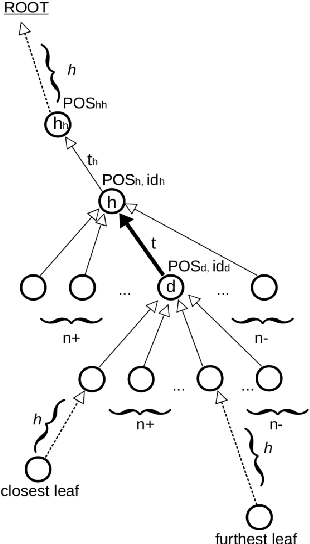
\includegraphics[scale=0.5]{img/lisca_stats.png}
    \caption[Features Used by LISCA to Calculate Plausibility Score for an Arc]{Features Used by LISCA to Calculate Plausibility Score for an Arc (marked in bold). Figure borrowed from \cite{alzetta2017dangerous}. }
\end{reusefigure}

The goal of the experiment is two-fold. For the low-resource languages, when there is no reference corpus, LISCA cannot be used directly. A common approach used in the case of low-resource languages, \(k\)-fold cross-validation is explored in this experiment. However, just using cross-validation is not enough, as the choice of the number of folds can affect the results significantly. In this experiment, we therefore (i) evaluate if \(k\)-fold cross-validation is an optimal strategy against the approach of keeping the test and train data separated, and (ii) try to map the behaviour of the algorithm to the choice of the number of folds in \(k\)-fold cross-validation approach.

In the following subsections, we shall elaborate on the experiment with LISCA. We start with the specification of the dataset to be used for the experiment in section \ref{data:lisca}, followed by the elaboration on experimental setup in section \ref{preprocess:lisca}. Section \ref{arcs:focus} specifies the manner of investigation for the analysis of arcs. We report the preliminary statistics on different runs in section \ref{baseline:lisca}, before diving into an analysis of the results in section \ref{compare:lisca}. Section \ref{typologies:lisca} deals with the typologies of errors discovered over the complete experiment. The chapter concludes with a discussion on the findings of the experiment in section \ref{results:lisca}.

\section{Dataset}
\label{data:lisca}

The experiment was conducted entirely on data from \verb|hi|-HDTB treebank from UDv2.4\footnote{Code alongwith manually annotated data is available at \url{https://github.com/Akshayanti/Masters-Thesis-CUNI-2020/tree/master/lisca_coldstart}} \citep{UDv2.4}. The motivation behind the limiting of the dataset to a particular language is threefold. Firstly, the treebank in question is limited to news genre. The lack of variability in the genre in the treebank can be used to frame a better statistical model than when there would be different genres present. Secondly, the treebank is medium sized (16,000+ sentences containing around 350k tokens) as can be seen in Table \ref{tab:hi_size2}. The medium sized treebank is optimal in the manner that a variety of values (of the number of folds in \(k\)-fold cross validation procedure) can be experimented with. Furthermore, the different values of the parameter can be used to ascertain the performance of the algorithm in both large-sized and small-sized treebanks. Lastly, the author has \verb|hi| as their native language, making it easier for them to analyse the given data, thus reducing the source of ambiguity during the process of manual annotation and verification of results from the results of the algorithm.

\begin{table}[H]
    \centering
    \begin{tabular}{|c|c|c|}
    \hline
    \textbf{Split} & \textbf{Sentences} & \textbf{Tokens}\\
    \hline
    \hline
    \textbf{dev} & 1 659 & 35 217\\
    \textbf{test} & 1 684 & 35 430\\
    \textbf{train} & 13 304 & 281 057\\
    \hline
    \hline
    \textbf{Total} & \textbf{16 647} & \textbf{351 704}\\
    \hline
    \end{tabular}
    \caption{Size of \texttt{hi}-HDTB treebank}
    \label{tab:hi_size2}
\end{table}

\section{Experimental Setup}
\label{preprocess:lisca}

For the remainder of the experiment, we adapt the usage of \textit{iteration} and \textit{run} as follows. The results of one \textit{run} would be analysed together. For a given \(k\) value in \(k\)-fold cross validation, the experimental data is split into \(k\) different folds, running \(k\) \textit{iterations} for one run. 

For the different runs of the current experiment, the total number of sentences poses a problem in the terms of how many folds the data can be split into\footnote{16,647 can be factorised as 3 x 31 x 179, which allows limited manipulation in the number of folds that can be worked with for equal distribution of instances.}. To combat this problem, we first concatenate the different splits of the treebank into one. The concatenated split is then downsampled to 16,000 sentences. This downsampled data becomes our functional dataset for the experiment. The downsampling is needed to allow for the different values of \(k\) to work. While the data if downsampled to 16,640 instances would have also worked, we chose to set the count to 16,000 sentences for empirical reasons. The number of sentences from the original splits that feature in the downsampled version are as listed in Table \ref{tab:split_lisca_downsample}.

\begin{table}[H]
    \centering
    \begin{tabular}{|l||c|c||c|c|}
    \hline
    \multicolumn{1}{|c||}{\textbf{Split Name}} &
    \multicolumn{2}{c||}{\textbf{Sentences}} &
    \multicolumn{2}{c|}{\textbf{Tokens}}\\
     & \textbf{Before} & \textbf{After} & \textbf{Before} & \textbf{After}\\
    \hline
    \textbf{dev} & 1 659 & 1 601 & 35 217 & 33 964\\
    \textbf{test} & 1 684 & 1 614 & 35 430 & 33 981\\
    \textbf{train} & 13 304 & 12 785 & 281 057 & 270 249\\
    \hline
    \hline
    \textbf{Total} & 16 647 & 16 000 & 351 704 & 338 194\\  
    \hline
    \end{tabular}
    \caption{Counts of Sentences and Tokens from Individual Splits, Before and After Downsampling}
    \label{tab:split_lisca_downsample}
\end{table}

\subsubsection{Setup for Baseline Run}

We call an arc as belonging to downsampled train data if (i) the arc was part of the train set in the original data, and (ii) the arc is present in the downsampled data as well. The arcs belonging to downsampled dev data and downsampled test data are also defined similarly.

For establishing a baseline, we train the algorithm on downsampled dev and downsampled train sets, concatenated together. The trained algorithm is then run against the downsampled test data to get the plausibility score of the individual arcs present therein.

\subsubsection{Setup for Experimental Runs}

The experiments were conducted on 3 different values of \(k\). The chosen values were \(k = \{2, 4, 8\}\). When the values of \( k \geq 10\) were considered, the resulting data folds became smaller enough to not yield satisfactory results.

For each value of \(k\), the cross-validation procedure was applied to get the plausibility scores for the arcs in the entire downsampled dataset. The LISCA algorithm for each iteration was run by \citeauthor{alzetta2017dangerous} separately. Algorithm \ref{algo:liscadata} summarises the procedure involved so far.

\begin{algorithm}[H]
\caption{Experimental Setup for \(k\)-fold Cross Validation}
\label{algo:liscadata}
    \begin{algorithmic}[1]
    \REQUIRE Downsampled \texttt{hi}-HDTB Treebank $T$
    \FORALL{$k$ in \{2, 4, 8\}}
        \STATE $T.folds \leftarrow \{T.1$, ..., $T.k\}$ subject to conditions:
        \STATE $T = \bigcup \{T.1, ..., T.k\}$ \COMMENT{Condition 1}
        \STATE $sentences(T.i) = sentences(T)/k \hspace{2mm} \forall T.i \in T$
        \COMMENT{Condition 2}
        \STATE $\bigcap \{T.x1, T.x2\} = \phi \hspace{2mm} \forall \{T.x1, T.x2\}  \in T.folds$ \COMMENT{Condition 3}
        \FOR{$iteration$ in 1, ..., k}
            \STATE $fold.test \leftarrow T.iteration$
            \STATE $fold.training \leftarrow T - T.iteration$
            \STATE $lisca.iteration \leftarrow$ trained LISCA model on $fold.training$
            \STATE $lisca.iteration$ is used to assign plausibility score to arcs in $fold.test$
        \ENDFOR
    \ENDFOR
    \end{algorithmic}
\end{algorithm}

\section{Arcs in Focus}
\label{arcs:focus}

The evaluation of a trained LISCA model on a given test data generates several types of statistics. In addition, the individual arcs in the results of the LISCA algorithm are split into 10 equal bins in descending order of their plausibility scores, with an additional bin for the remnants. The statistics are presented on a per-bin basis and include POS distribution, deprel distribution, POS and deprel distribution, syntactic link length distribution, among others. While the per-bin statistics are a useful feature, the cross validation process in the context of current experiment does not need such per-bin statistics. Instead we focus on individual arcs and their plausibility scores in the current experiment.

Henceforth, we call a particular arc as flagged in a particular run if its plausibility score in the run is designated as 0, i.e. the arc is deemed as improbable by the run. While \cite{alzetta2017dangerous} looked at all the instances in the last two bins (and the extra remnant bin), the current setup narrows down the search scope. The last two (and the extra remnant) bins in question are the only ones containing arcs with 0-score or with scores that are very close to 0. As we would show later (in section \ref{statistics:experiments}), the scores for non-zero scored arcs would fluctuate with different datasets of the same language, or even based on the number of folds in cross validation. This can be extrapolated to state that the non-zero scored arcs in the bins in question can also vary in their scores, making the bin-specific treatment incomparable across different runs. In contrast, looking at zero-scored arcs gives us a uniform base for analysis throughout, considering that the arc was marked as improbable, and not probable with a low score.

\section{Statistics}
\label{baseline:lisca}

\subsection{Baseline Run}
\label{statistics:baseline}

The baseline run tried to find the low-probability arcs in the downsampled test data. Table \ref{tab:stats_baseline} shows the basic statistics of the run.

\begin{table}[H]
    \centering
    \begin{tabular}{|l|l|}
        \hline
        \textbf{Statistic} & \textbf{Count / Value} \\
        \hline
        Min Score & 0.00\\
        Max Score & 1.82 E-07\\
        Flagged Arcs (in \%) & 221 (0.7 \%)\\
        Total Arcs & 33 739\\
        \hline
    \end{tabular}
    \caption[Statistics for Arc Scores in Baseline Run]{Statistics for Arc Scores in Baseline Run. The percentage score of Flagged Arcs is calculated against the Total Arcs count.}
    \label{tab:stats_baseline}
\end{table}

Once the plausibility scores are assigned for the arcs, the flagged arcs were manually checked to see if they are erroneous or not. Of the 221 flagged arcs in the run, 110 arcs were found to be erroneous. The complete typology of the errors is reserved for later. However, Table \ref{tab:base_error_breakdown} shows the classification of errors from the run into Random or Systemic Errors.

\begin{table}[H]
    \centering
    \begin{tabular}{|l|c|}
        \hline
        \textbf{Statistic} & \textbf{Count (\% Total Arcs)}\\
        \hline
        No Error & 111 (49.3 \%)\\
        Systemic Errors & 96 (43.4 \%)\\
        Random Errors & 14 (6.3 \%)\\
        Total Flagged Arcs & 221\\
        \hline
    \end{tabular}
    \caption{Classification of Errors in Baseline Run}
    \label{tab:base_error_breakdown}
\end{table}


\subsection{Experimental Runs}
\label{statistics:experiments}

Table \ref{tab:absminmax} shows the number of arcs that were flagged across different experimental runs. As mentioned earlier, the maximum plausibility score of arcs in a given run fluctuates with the different \(k\)-values across different runs, even when the overall experimental data remains the same.

\begin{table}[H]
    \centering
    \begin{tabular}{|c|c|c|c|c|}
    \hline
    \textbf{\(k\)-value} & \textbf{Min Score} & \textbf{Max Score} & \textbf{0-score arcs} & \textbf{Total arcs}\\
    \hline
    \hline
    2 & 0.00 & 1.96 E-07 & 3 487 & 336 079 \\
    4 & 0.00 & 1.93 E-07 & 2 620 & 336 079 \\
    8 & 0.00 & 1.91 E-07 & 2 319 & 336 079 \\
    \hline
    \end{tabular}
    \caption{Statistics for Arc Scores in Experimental Runs}
    \label{tab:absminmax}
\end{table}

The number of 0-scored arcs went down with an increasing \(k\)-value. In addition, all the arcs flagged in a particular run were also present in a run with a lower \(k\)-value, i.e. the arcs flagged in run with \(k=4\) were also present in \(k=2\). Similarly, the arcs flagged in run with \(k=8\) were present in the run with \(k=4\) as well as one with \(k=2\). We compare the performance of the different experimental runs against each other in section \ref{analysis:all}.

\section{Analysis}
\label{compare:lisca}

In this section, we analyse the experiment in two parts. In the first part of the analysis (Section \ref{analysis:test}), we check the usefulness of \(k\)-fold cross validation against the arcs from only the downsampled test data, comparing them at the same time. The primary motive of this analysis is to understand how the cross validation technique performs in relation to the baseline approach at identifying erroneous instances in a low-resource setting.

In the second part of the analysis (Section \ref{analysis:all}), we look at all the arcs that are flagged in different cross validation runs, regardless of them belonging to the downsampled test, dev or train data. The motive of this analysis is to understand how the difference in number of folds during cross validation affects the flagged instances.

\subsection{Baseline vs Cross Validation: Who did it better?}
\label{analysis:test}

Table \ref{tab:test_lisca} shows the number of test arcs that were flagged across different cross validation runs. The values in the last column represent the count of instances that were flagged by the experimental run as well as the baseline run. 

\begin{table}[H]
    \centering
    \begin{tabular}{|c||c|c|c|c|}
    \hline
    \multicolumn{1}{|c||}{\textbf{\(k\)-value}} &
    \multicolumn{1}{c|}{\textbf{\# Flagged}} &
    \multicolumn{1}{c|}{\textbf{\# Also Flagged by Baseline}}\\
     & & \textbf{(\% \# Flagged)}\\
    \hline
    2 & 333 & 211 (63.36\%) \\
    4 & 254 & 205 (80.71\%) \\
    8 & 226 & 205 (90.71\%) \\
    \hline
    \end{tabular}
    \caption{Commonly Flagged Instances from Downsampled Test Data in Baseline and Experimental Runs}
    \label{tab:test_lisca}
\end{table}

Table \ref{tab:baseline_cv_error_percentage} shows the counts of arcs in downsampled test data that were flagged across different runs, and the count of flagged arcs that were erroneous.

\begin{table}[H]
    \centering
    \begin{tabular}{|c|c|c|c|}
    \hline
    \textbf{Run} & \textbf{\# Flagged} & \textbf{\# Errors} & \textbf{Error Precision (in \%)}\\
    \textbf{ } & \textbf{(TP+FP)} & \textbf{TP} & \textbf{TP*100/(TP+FP)}\\
    \hline
    Baseline & 221 & 109 & 49.32 \%\\
    Experimental (\(k=2\)) & 333 & 160 & 48.05 \%\\
    Experimental (\(k=4\)) & 254 & 127 & 50.00 \%\\
    Experimental (\(k=8\)) & 226 & 114 & 50.44 \%\\
    \hline
    \end{tabular}
    \caption{Error Counts in Downsampled Test Data across Different Runs}
    \label{tab:baseline_cv_error_percentage}
\end{table}

Table \ref{tab:baseline_cv_error_percentage} can be analysed in two different ways. The first analysis would focus on the error precision for each run. We notice that an increase in \(k\)-value in cross-validation approach results in an increasing precision. While the experimental run with \(k=2\) had a precision lower than the precision of the baseline run (\(\Delta = -1.27 \%\)), the other experimental runs had a higher precision than the baseline run (\(\Delta = 0.68 \%\) for \(k=4\) and \(\Delta = 1.12 \%\) for \(k=8\)). In this aspect, cross-validation technique still outperforms the trivial technique used in the baseline task. However, the choice of \(k\)-value in this case needs to be monitored for a higher precision.

The second analysis of data in Table \ref{tab:baseline_cv_error_percentage} would essentially focus on the number of identified erroneous arcs in the individual run. Considering that we are interested in a higher number of error arcs, either of the experimental runs outperform the baseline task in that aspect as well.

We therefore are able to establish that the cross-validation technique is a better choice than the trivial approach. Table \ref{tab:typology_test_arcs} shows the typology of different errors as identified in the different runs. We discuss the most relevant error typologies in Section \ref{typologies:lisca}.

\begin{table}[H]
    \scalebox{0.95}{\begin{tabular}{|l|c|c|c|c|}
    \hline
    \textbf{Error Typology} & \textbf{Baseline} & \textbf{\(k=2\)} & \textbf{\(k=4\)} & \textbf{\(k=8\)}\\
    \hline
        \texttt{advcl4advmod} & 2 (0.9\%) & 2 (0.6\%) & 2 (0.8\%) & 2 (0.9\%)\\
        \texttt{advcl4det} & - & 2 (0.6\%) & - & -\\
        \texttt{amod4acl} & 2 (0.9\%) & 3 (0.9\%) & 2 (0.8\%) & 2 (0.8\%)\\
        \textbf{\texttt{amod4xcomp}} & 2 (0.9\%) & 3 (0.9\%) & 3 (1.2\%) & 2 (0.9\%)\\
        \texttt{compound4det} & - & 2 (0.6\%) & 1 (0.4\%) & 1 (0.4\%)\\
        \texttt{compound4obj} & 1 (0.5\%) & 2 (0.6\%) & 2 (0.8\%) & 2 (0.9\%)\\
        \textbf{\texttt{nmod4obl}} & - & 4 (1.2\%) & 2 (0.8\%) & 1 (0.4\%)\\
        \textbf{\texttt{obl4advcl|acl}} & 1 (0.5\%) & 2 (0.6\%) & 2 (0.8\%) & 1 (0.4\%)\\
        \texttt{obl4discourse|mark} & - & 3 (0.9\%) & 1 (0.4\%) & -\\
        \texttt{Case Error} & 5 (2.3\%) & 6 (1.8\%) & 5 (2.0\%) & 5 (2.2\%)\\
        \texttt{MWE Error} & 5 (2.3\%) & 5 (1.5\%) & 5 (2.0\%) & 5 (2.2\%)\\
        \texttt{Naming Error} & 9 (4.1\%) & 11 (3.3\%) & 9 (3.5\%) & 8 (3.5\%)\\
        \texttt{POS Error} & 5 (2.3\%) & 5 (1.5\%) & 3 (1.2\%) & 3 (1.3\%)\\
        \texttt{Reported Speech} & 4 (1.8\%) & 2 (0.6\%) & 2 (0.8\%) & 2 (0.9\%)\\
        \texttt{Tree Error} & 20 (9.0\%) & 29 (8.7\%) & 25 (9.8\%) & 22 (9.7\%)\\
        \texttt{Wrong Head} & 38 (17.2\%) & 54 (16.2\%) & 42 (16.5\%) & 40 (17.7\%)\\
        Random Errors & 15 (6.8\%) & 25 (7.5\%) & 21 (8.3\%) & 18 (8.0\%)\\
        No Error & 112 (50.7\%) & 173 (50.0\%) & 127 (50.0\%) & 112 (49.6\%)\\
    \hline
        \textbf{Total Flagged Arcs} & \textbf{221} & \textbf{333} & \textbf{254} & \textbf{226}\\
    \hline
    \end{tabular}}
    \caption[Typology of Errors in Downsampled Test Data across Different Runs]{Typology of Errors in Downsampled Test Data across Different Runs. Percentages are calculated against the Total number of Flagged Arcs in the Run. Error Typologies marked in bold have been previously pointed out by \cite{alzetta2017dangerous}}
    \label{tab:typology_test_arcs}
\end{table}

\subsection{Comparing Different Experimental Runs}
\label{analysis:all}

For the analysis of the different cross-validation runs, we noticed that the count of flagged instances decreased with the increase in the number of folds. We hypothesise that as we increase the number of folds, the detection of rare errors improves while the detection of frequent errors deteriorates. having noted this, we analysed the effect of each k-value in the following manner. For the 0-scored arcs that were common to all the runs, 200 randomly chosen arcs (out of 2319) were evaluated manually. Out of the arcs common only to the runs corresponding to \(k= \{2, 4\}\), 100 were randomly chosen for manual evaluation. Finally, 100 of the arcs that are local only to the run corresponding to \(k=2\) were chosen randomly for manual evaluation. The manual evaluation on a flagged instance was meant to classify if the flagged instance is indeed an error, and if so, of what kind.

The manual annotation on limited subsamples as above does not offer a comparative viewpoint of the performance of the different runs. To combat this, we estimate the normalized frequency of each error type over 1000 instances in Table \ref{tab:normalized_experimental_lisca}. The values are calculated as per the equation given below. The equation normalizes the frequency of an error over 1000 flagged arcs, based on the distribution of the error in the annotated samples.

    \[f_{error} = 
    \begin{cases}
    k_{2,4,8} \cdot 5 &\text{for }k=8\\
    \vspace{2mm}\\
    \left[ \frac{k_{2,4,8} \cdot 2319}{200} + \frac{k_{2,4} \cdot 311}{100} \right] \cdot \frac{1000}{2620} & \text{for }k=4\\
    \vspace{2mm}\\
    \left[ \frac{k_{2,4,8} \cdot 2319}{200} + \frac{k_{2,4} \cdot 311}{100} + \frac{k_{2} \cdot 867}{100} \right] \cdot \frac{1000}{3487} & \text{for }k=2
    \end{cases}\]
where
\begin{itemize}
    \item \(f_{error}\) represents the normalised frequency of \(error\)
    \item \(k_{2,4,8}\) represents the counts of \(error\) in the annotated sample of arcs commonly flagged by all the experimental runs
    \item \(k_{2,4}\) represents the counts of \(error\) in the annotated sample of arcs commonly flagged by runs with \(k=2\) or \(k=4\), but not flagged by run with \(k=8\)
    \item \(k_{2}\) represents the counts of \(error\) in the annotated sample of arcs flagged only by the run with \(k=2\), but not flagged by runs with \(k=4\) or \(k=8\)
\end{itemize}

\begin{table}[H]
    \centering
    \begin{tabular}{|l|c|c|c|}
        \hline
        \textbf{Error Typology} & \textbf{\(k = 2\)} & \textbf{\(k= 4\)} & \textbf{\(k=8\)} \\
        \hline
        \texttt{advmod4amod} & 7 & 9 & 10\\
        \texttt{dep4det} & 6 & 8 & 5\\
        \texttt{dep4discourse|mark} & 6 & 5 & 5\\
        \texttt{nsubj4obj} & 8 & 7 & 5\\
        \textbf{\texttt{obl4advcl|acl}} & 6 & 8 & 5\\
        \texttt{Case Error} & 16 & 8 & 5\\
        \texttt{MWE Error} & 15 & 13 & 15\\
        \texttt{Naming Error} & 43 & 51 & 50\\
        \texttt{POS Error} & 10 & 13 & 15\\
        \texttt{Reported Speech} & 12 & 13 & 15\\
        \texttt{Tree Error} & 47 & 61 & 60\\
        \texttt{Wrong Head} & 163 & 167 & 180\\
        Random Errors & 142 & 115 & 115\\
        No Error & 519 & 522 & 515\\
        \hline
        \textbf{Total Errors} & \textbf{481} & \textbf{478} & \textbf{485}\\
\hline
    \end{tabular}
    \caption[Error Frequencies for Experimental Runs, Normalized Over 1000 Flagged Arcs]{Error Frequencies for Experimental Runs, Normalized Over 1000 Flagged Arcs. Error Typologies marked in bold have been previously pointed out by \cite{alzetta2017dangerous}}
    \label{tab:normalized_experimental_lisca}
\end{table}

Perhaps the most striking result from Table \ref{tab:normalized_experimental_lisca} is how the different experimental runs are almost similar in their performance. Notice that in Table \ref{tab:baseline_cv_error_percentage}, an increase in number of folds was accompanied by an increase in the calculated error precision. The analysis in the two cases is different. While in Table \ref{tab:baseline_cv_error_percentage} we checked if using the cross-validation to train the algorithm has any significant performance gain; the results in Table \ref{tab:normalized_experimental_lisca} analyzes if the number of folds has any correlation with error-detection rate when there is no reference corpus, and the algorithm is trained and tested on the same data. 

Since the number of folds in cases when the algorithm is trained and tested using cross-validation has little to no effect in performance gain, the only point of differentiation between different runs is with respect to the number of flagged arcs. While it is lucrative to use less number of folds (or a lower \(k\) value), the approach would be bottle-necked by the size of the dataset.

An error type is considered significant if its normalized frequency is more than 1\% (frequency \(> 10\)) in  Table \ref{tab:normalized_experimental_lisca}. We discuss the significant error types in the next section.

\section{Error Typologies}
\label{typologies:lisca}

In this section, we elaborate on the error typologies discovered throughout the scope of the experiment such that the discovered error type is present in more than 1\% of the arcs flagged in any run, baseline or experimental. The focused errors in this section include: \texttt{Case Error}, \texttt{MWE Error}, \texttt{Naming Error}, \texttt{Reported Speech}, \texttt{Tree Error} and \texttt{Wrong Head}. Since `Random Errors' are not systemic in nature, we do not elaborate on them. Additionally, \texttt{POS Error} corresponds to an error in the POS annotation label, and is not elaborated upon any further in this section.

\subsection[Identification Error of Case-Marker: \texttt{Case Error}]{\texttt{Case Error}: Identification Error of Case-Marker}

In \texttt{hi}, the different grammatical cases are more often than not marked by case-marker tokens. This error corresponds to such case-markers being marked by deprels other than \texttt{case}. Additionally, the deprel is the preferred choice for constructions that involve possessions as well. In the event that the used deprel is other than \texttt{case}, we call it as \texttt{Case Error}.

Part of sentence from UDv2.4 \texttt{hi}-HDTB treebank in Example \ref{examp:caseError}, and the associated dependency tree in Figure \ref{examp:caseError-fig} highlights the error type. The token of interest is marked in bold.

\begin{example}
\label{examp:caseError}
\textbf{ }\\
\textbf{Text (\texttt{hi}):} \texthindi{मार्क्र्सवादी कम्युनिस्ट पार्टी ( माकपा ) \textbf{के} दस सांसदों}\\
\textbf{Translit:} \textit{Marx-vaadi Communist Party ( MaCPa ) \textbf{ke} das saansadon}\\
\textbf{Lit.:} Marxist Communist Party (MaCPa) \textit{Poss.} ten senator-\textit{Acc.}-\textit{Pl.}\\
\textbf{Translated:} 10 senators of Marxist Communist Party (MaCPa)
\end{example}

\begin{figure}[H]
    \centering
    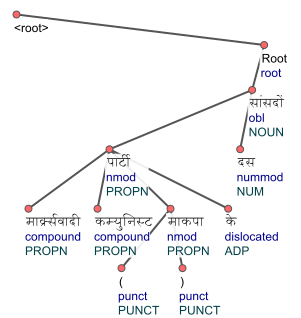
\includegraphics[scale=0.90]{img/caseError.png}
    \caption{\texttt{Case Error} in Example \ref{examp:caseError}}
    Note: Root is used as a placeholder for root of the tree\\
    Note: \texthindi{मार्क्र्सवादी} (\textit{Marx-vaadi}; Marxist) should be attached to \texthindi{पार्टी} (\textit{Party}; Party) using deprel \texttt{flat}, and not with \texttt{compound}\\
    Note: \texthindi{कम्युनिस्ट} (\textit{Communist}; Communist) should be attached to 
    \texthindi{पार्टी} (\textit{Party}; Party) using deprel \texttt{flat}, and not with \texttt{compound}\\
    Note: \texthindi{माकपा} (\textit{MaCPa}; abbreviation of Marxist Communist Party) should be attached to 
    \texthindi{पार्टी} (\textit{Party}; Party) using deprel \texttt{appos}, and not with \texttt{nmod}\\
    Note: \texthindi{के} (\textit{ke}; \textit{Poss.}) should be attached to 
    \texthindi{पार्टी} (\textit{Party}; Party) using deprel \texttt{case}, and not with \texttt{dislocated}
    
    \label{examp:caseError-fig}
\end{figure}
% test-s957
\newpage

\subsection[Annotation Error in Multi-Word Expression (MWE): \texttt{MWE Error}]{\texttt{MWE Error}: Annotation Error in Multi-Word Expression (MWE)}

The different tokens in a Multi-Word Expression (MWE) are combined by either of the deprels in UDv2: \texttt{fixed}, \texttt{compound} or \texttt{flat}. Of these, \texttt{fixed} is used for completely fixed grammaticized (function word-like) MWEs (like `in spite of'), and \texttt{compound} applies to endocentric (headed) MWEs (like `apple pie').

The usage of \texttt{fixed} deprel is covered separately in \texttt{Naming Error}. For instances when a MWE should be annotated as either of \texttt{compound} or \texttt{fixed} deprels, but is annotated otherwise, we refer to the error as \texttt{MWE Error}. Example \ref{examp:mweError} shows the error type in a sentence from UDv2.4 \texttt{hi}-HDTB treebank, with the associated dependency tree in Figure \ref{examp:mweError-fig}. The MWE is marked in bold.

\newpage
\begin{example}
\label{examp:mweError}
\textbf{ }\\
\textbf{Text (\texttt{hi}):} \texthindi{इसकी सबसे बड़ी विशेषता यह है कि सामान्य कार्य चलता रहेगा और किसी चीज की प्रोसेसिंग भी \textbf{अपने आप} होती रहेगी ।}\\
\textbf{Translit:} \textit{iski sabse badi visheshta yeh hai ki saamaanya kaarya chaltaa rahegaa aur kisi cheej ki processing bhi \textbf{apne aap} hoti rahegi.}\\
\textbf{Lit.:} \textcolor{red}{\textit{3P.Poss.} \textit{Superlative} big feature this is that normal work run-\textit{Imp.} \textit{Fin.} and some thing \textit{Poss.} process also by-itself}\\
\textbf{Translated:} \textcolor{red}{Need to ask for translation}
\end{example}

\begin{figure}[H]
    \centering
    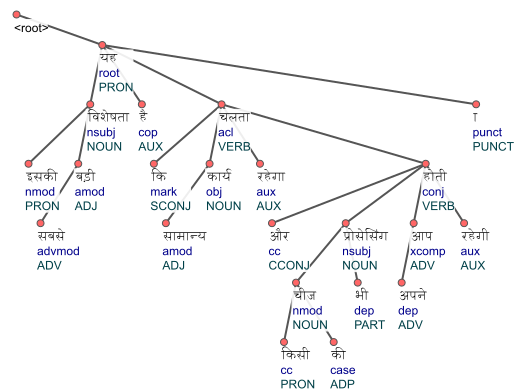
\includegraphics[scale=0.90]{img/mweError.png}
    \caption{\texttt{MWE Error} in Example \ref{examp:mweError}}
    Note: \texthindi{अपने} (\textit{apne}; ?) should be connected to \texthindi{आप} (\textit{aap}; ?) using deprel \texttt{fixed}, and not \texttt{dep}
    \label{examp:mweError-fig}
\end{figure}
% train-s1411

\subsection[Annotation Error in Construction With Reported Speech: \texttt{Reported Speech}]{\texttt{Reported Speech}: Annotation Error in Construction With Reported Speech}

According to UDv2 guidelines for treatment of reported speech\footnote{\url{https://universaldependencies.org/u/dep/parataxis.html\#treatment-of-reported-speech}}, the reported speech is connected to the main clause by using either of the deprel \texttt{ccomp} or \texttt{parataxis}.

The error \texttt{Reported Speech} corresponds to case when the reported speech and main clause are not connected by proper deprels, as in the example from UDv2.4 \texttt{hi}-HDTB treebank.

\begin{example}
\label{examp:reportedSpeech}
\textbf{ }\\
\textbf{Text (\texttt{hi}):} \texthindi{समिति ने कहा था कि सभी संस्थान मौजूदा आईआईटी के स्तर की तुलना में काफी पीछे हैं ।}\\
\textbf{Translit:} \textit{samiti ne kahaa thaa ki sabhi sansthaan maujoodaa IIT ke star ki tulnaa mei kaafi peeche hain.}\\
\textbf{Lit.:} Committee \textit{Acc.} say be-\textit{Perf.} that all institutes present IIT \textit{Poss.} level in-comparison-with quite behind is-\textit{Pl.} . \\
\textbf{Translated:} Committee had said that all institutes are far behind the level of the current IITs. 
\end{example}

\begin{figure}[H]
    \centering
    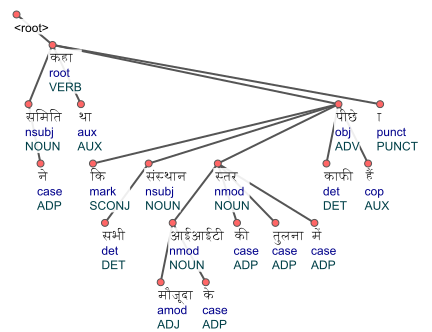
\includegraphics[scale=0.90]{img/reportedSpeech.png}
    \caption{\texttt{Reported Speech Error} in Example \ref{examp:reportedSpeech}}
    Note: \texthindi{पीछे} (\textit{peeche}; behind) should be attached to 
   \texthindi{कहा} (\textit{kaha}; say) using the deprel \texttt{ccomp}
    \label{examp:reportedSpeech-fig}
\end{figure}
% test-s1055

\subsection[Head Identification Error: \texttt{Wrong Head}]{\texttt{Wrong Head}: Head Identification Error}

The error refers to the cases when the dependent in the flagged arc is attached to a wrong head. This is the umbrella error type for all the cases of head identification error that cannot be categorised more specifically into other error types.

While \cite{alzetta2017dangerous} mention head labelling error as a sub-type of the error patterns discussed therein, we identify this error in a category on its own. We separate this error type because multiple parsers/taggers determine the deprel of a dependent in an arc based on the head of the said dependent. Keeping this in mind, \texttt{Wrong Head} is very likely to result in a faulty deprel annotation as well. However, attachment to the correct head in this case should essentially result in a correction of the annotated deprel as well.

Consider Example \ref{examp:wrongHead} and the associated dependency tree in Figure \ref{examp:wrongHead-fig}. The example is part of a sentence taken from the UDv2.4 \texttt{hi}-HDTB treebank, and shows the token of interest (marked in bold) attached to a wrong head.

\begin{example}
\label{examp:wrongHead}
\textbf{ }\\
\textbf{Text (\texttt{hi}):} \texthindi{जिनकी \textbf{मदद} से \textbf{वह आवाज} को पहचान व समझ सकता है}\\
\textbf{Translit:} \textit{jinki \textbf{madad} se \textbf{vah aavaaz} ko pehchaan va samajh saktaa hai}\\
\textbf{Lit.:} whose help \textit{Acc.} it sound \textit{Acc.} recognise and understand can is\\
\textbf{Translated:} With help of which, it can recognise and understand sound.
\end{example}

\begin{figure}[H]
    \centering
    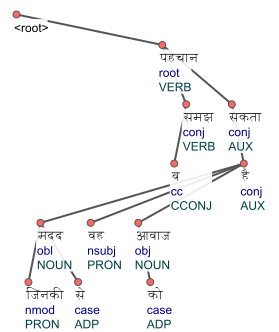
\includegraphics[scale=0.90]{img/wrongHead.png}
    \caption{Head Identification Error in Example \ref{examp:wrongHead}}
    Note: \texthindi{मदद} (\textit{madad}; help) should be attached to \texthindi{पहचान} (\textit{pehchaan}; recognise) and not to \texthindi{है} (\textit{hai}; is)\\
    Note: \texthindi{वह} (\textit{vah}; it) should be attached to \texthindi{पहचान} (\textit{pehchaan}; recognise) and not to \texthindi{है} (\textit{hai}; is)\\
    Note: \texthindi{आवाज} (\textit{aavaz}; sound) should be attached to \texthindi{पहचान} (\textit{pehchaan}; recognise) and not to \texthindi{है} (\textit{hai}; is)\\
    \label{examp:wrongHead-fig}
\end{figure}
% test-s1083

\subsection[Annotation Error in Proper Nouns: \texttt{Naming Error}]{\texttt{Naming Error}: Annotation Error in Proper Nouns}

\texttt{Naming Error} is often accompanied with a head-identification error. Annotation Errors in Proper Nouns can be of three kinds, and all of these are commonly grouped under \texttt{Naming Error}. The following are the possible cases of error in annotation:

\begin{enumerate}

    \item \textbf{Proper Noun as Appositional Modifier} (\texttt{4appos}): The deprel \texttt{appos}\footnote{\url{https://universaldependencies.org/u/dep/appos.html}} is used when the proper noun defines, modifies, names or describes a preceding nominal. It also includes parenthesized examples, and the abbreviations. This error is characterized by an attempt to connect the two nominals by relations such as \texttt{nmod}, when the actual deprel should be \texttt{appos}.
    
    \item \textbf{Names/Dates without Syntactic Structure} (\texttt{4flat}): The different parts of a single name, or of a date should be attached to the head with the deprel \texttt{flat}\footnote{\url{https://universaldependencies.org/u/dep/flat.html}}. The deprel is also used in cases of a honorofic or a title. This error type is characterized by usage of other deprels when \texttt{flat} should be the deprel of choice.

    \item \textbf{Names with Syntactic Structure}: Names that follow a syntactic structure (like `A Tale of Two Cities') should not be annotated with \texttt{flat} deprel, but with regular syntactic relations. In this case, the error is characterized by a name with syntactic structure being analysed in the same way as a name without syntactic structure.
    
\end{enumerate}

Consider the part of a sentence from UDv2.4 \texttt{hi}-HDTB treebank showcasing all the above cases in Example \ref{examp:namingError} and the associated dependency tree in Figure \ref{examp:namingError-fig}
\begin{example}
\label{examp:namingError}
\textbf{ }\\
\textbf{Text (\texttt{hi}):} \texthindi{आरसी मिश्रा की पुस्तक 'मानवाधिकार संरक्षण विशेष संदर्भ, अपराधियों का निरोध एवं उपचार'}\\
\textbf{Translit:} \textit{Aarsi Mishra ki pustak ` Maanavadhikar sanrakshan vishesh sandarbh , apraadhiyon ka nirodh evam upchaar '}\\
\textbf{Lit.:} Aarsi Mishra \textit{Poss.} book ` Human-Rights Protection Special Reference , criminal-\textit{Pl.} \textit{Acc.} prevention and cure '\\
\textbf{Translated:} Aarsi Mishra's book, `Maanavadhikar sanrakshan vishesh sandarbh , apraadhiyon ka nirodh evam upchaar'
\end{example}

\begin{figure}[H]
    \centering
    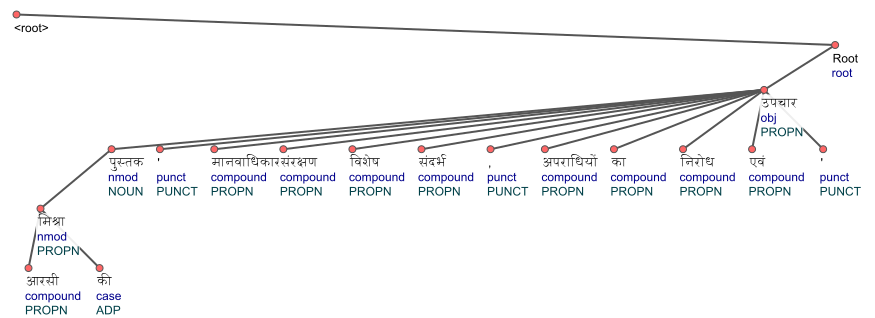
\includegraphics[scale=0.60]{img/namingError.png}
    \caption{\texttt{Naming Error} in Example \ref{examp:namingError}}
    Note: Root is used as a placeholder for root of the tree\\
    Note: \texthindi{आरसी} (\textit{Aarsi}; Aarsi) should be attached to \texthindi{मिश्रा} (\textit{Mishra}; Mishra) using deprel \texttt{flat}, and not with \texttt{compound}\\
    Note: The title of the book (limited by quotes) should be attached to \texthindi{पुस्तक} (\textit{pustak}; book) with the deprel \texttt{appos}\\
    Note: The title of the book (limited by quotes) should be annotated with regular syntactic relations
    \label{examp:namingError-fig}
\end{figure}
% test-s1183

\subsection[Dependency Head Located in Subtree: \texttt{Tree Error}]{\texttt{Tree Error}: Dependency Head Located in Subtree}

A special case of \texttt{Wrong Head} error, this error type is used for the cases when the actual head of a dependency is located inside the subtree rooted at the dependent. In order to correct the dependency, it should be essentially inverted. Essentially speaking, a tree marked with this error type requires re-annotation before any analysis can be performed on it.

Example \ref{examp:treeError} shows an instance of this error in UDv2.4 \texttt{hi}-HDTB treebank, with the associated dependency tree in Figure \ref{examp:treeError-fig}. The dependent of interest is marked in bold, and the corrected instance is as shown in Figure \ref{examp:treeError-fig2}.
\begin{example}
\label{examp:treeError}
\textbf{ }\\
\textbf{Text (\texttt{hi}):} \texthindi{आतंकियों द्वारा किसी विमान के \textbf{अपहरण} या आत्मघाती हमले को अंजाम देने की कोशिश किए जाने की खुफिया जानकारी}\\
\textbf{Translit:} \textit{aatankiyon dwara kisi vimaan ke \textbf{apharan} ya aatmghaati hamle ko anjaam dene ki koshish kiye jaane ki khufiya jaankaari}\\
\textbf{Lit.:} Terrorists by some plane \textit{Poss.} kidnap or self-harm attack \textit{Dat.} fruition give \textit{Dat.} attempt ? ? confidential information\\
\textbf{Translated:} The confidential information of attempt at some plane hijacking or suicide bombing by terrorists ...
\end{example}

\begin{figure}[H]
    \centering
    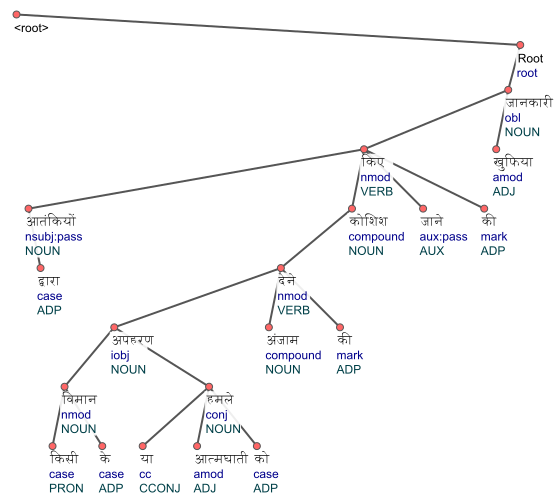
\includegraphics[scale=0.7]{img/treeError.png}
    \caption{\texttt{Subtree Error} in Example \ref{examp:treeError}}
    \label{examp:treeError-fig}
    Note: Root is used as a placeholder for root of the tree
\end{figure}

\begin{figure}[H]
    \centering
    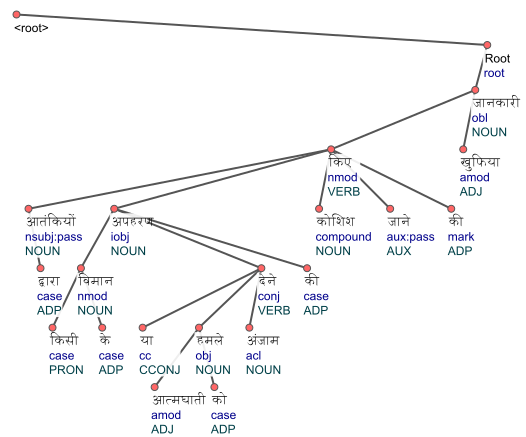
\includegraphics[scale=0.7]{img/treeError2.png}
    \caption{Correction of \texttt{Subtree Error} in Example \ref{examp:treeError}}
    \label{examp:treeError-fig2}
    Note: Root is used as a placeholder for root of the tree
\end{figure}
% dev-s1501

\section{Results and Discussion}
\label{results:lisca}

\subsection{0-scored Arcs as Search Criteria}

In their work, \cite{alzetta2017dangerous} focused on a total of 39.7k arcs in their annotation process and were finally able to manually revised 789 arcs, giving an estimated error detection rate of 2\% from the flagged instances. In our baseline run, a focus on 221 0-scored arcs led to an estimated error detection of 109 instances (49.32 \%). We must stress here that the results across the two experiments are NOT directly comparable since the treebanks used in the cited authors' experiment was of far superior quality than the one used in the current experiment. A lower quality treebank would imply a higher distribution of errors, and that could be the sole reason why the focus on a smaller subset gave a satisfactory error detection rate. Additionally, the size difference in the cited authors' work and the baseline task is another reason why the two approaches cannot be compared. We must also stress here that in our baseline approach, the search scope was lowered significantly (as compared to the experimental runs). To establish any significant difference between either approach, more experiments should be conducted with the same treebank (ensuring the quality of experimental data is a controlled variable) to establish the probability distribution of errors in 0-scored arcs and in the approach as utilised by \citeauthor{alzetta2017dangerous}.

\subsection{Cross Validation as Strategy}

Considering that the different runs perform almost similarly (Table \ref{tab:normalized_experimental_lisca}), we argue that the size of dataset used is the determining factor in selection of the number of folds in \(k\)-fold cross validation.

For less number of folds (or a lower \(k\) value), the number of flagged arcs is high, which eventually results in more errors detected. However, in case of a small dataset, the algorithm might be trained poorly if the number of folds is small. Thus, a higher number of folds (or a higher \(k\) value) is more optimal when the dataset is small in size. As the reference dataset size grows, lesser number of folds can be tried given that the algorithm can be trained well.

\subsection{Error Typologies and Annotation}

The annotations throughout the experiment were done by a single annotator. Even though inter-annotation inconsistency is a constant problem, the annotations done by a single author are even more prone to errors. While the annotations were checked multiple times, the possibility of annotation inconsistencies in manual annotation for error labelling cannot be discounted.

It is very likely for a single dependency arc to have an error that is defined separately under different labels. In such an event, the primary source of error was labelled as the error type. For example, if a dependency arc has \textit{Case Error} as well as \textit{Wrong Head} error, the former is very likely being caused by the latter. Therefore, the manual annotation for this instance would list it as a case of \textit{Wrong Head}.

Under the different head identification errors, the annotation was in the following order of priority, arranged in descending order:

\begin{enumerate}
    \item \texttt{MWE Error} or \texttt{Naming Error}
    \item \texttt{Tree Error}
    \item \texttt{Wrong Head}
\end{enumerate}

In essence, if the head identification error could not be localised to a specific error type, it was labelled under the umbrella error label of \texttt{Wrong Head}.

\subsection{Conclusion}

In the experiment, we narrowed the search scope from the bins as used by \cite{alzetta2017dangerous} to focus on the arcs that were considered as improbable by the algorithm. Additionally, we found that using cross-validation to train the algorithm has no significant performance gain.

For low-resource languages with little to no reference corpus data, we tried cross-validation approach for finding the errors. We discovered that the choice of folds in cross-validation strategy is determined by the size of the reference corpus; and in case of unavailability of one, the strategy can be used on the data itself without a significant loss in the error-detection rate.  % 17 pages on LISCA
    \chapter{\texttt{AUX} vs. \texttt{VERB}: Attempt at Separation of Verbs and Auxiliary Verbs (Experiment 4)}
\label{chap:failures}

We earlier mentioned how the line of distinction between verbs (POS tag \texttt{VERB}) and auxiliary verbs (POS tag \texttt{AUX}) is not well-defined in Section \ref{ssec:AuxVERB}. We shall treat this problem in this section, with a glance through some of the observations on the problem in Section \ref{ssec:auxverbsObservations}, followed by the definition of the working dataset in Section \ref{ssec:auxverbDataset}. We elaborate on the proposed solution to the problem, and the results of the experiment in Section \ref{ssec:auxverbExperiment} and \ref{ssec:auxverbResults} respectively. We finally conclude this section with a discussion of the results in \ref{ssec:auxverbDiscussion}.

\section{Observations About Problem Statement}
\label{ssec:auxverbsObservations}

According to the definition in UD\footnote{\url{https://universaldependencies.org/kpv/pos/AUX\_.html}}, \verb|AUX| is used as a common POS tag for verbal auxiliaries, as well as non-verbal TAME markers. The class of copulas are also included in this list.

This definition of auxiliaries is a bit different from \cite{langtypology} which separates the two classes of auxiliaries and copulas in different categories. The work also points out the correlation between the position of an inflected auxiliary in relation to the verb, and other word properties of the language, as first pointed by \cite{greenberg1963some}. In his work, \citeauthor{greenberg1963some} notes that the position of an inflected auxiliary in relation to the verb is generally the same as the position of verb in relation to an object. It is important to note that this generalization only holds for the inflected auxiliaries, and thus languages where the auxiliaries are not inflected are automatically ruled out from the consideration. \citeauthor{langtypology} points out the well-known exception to this generalization in case of verb-second languages like those of \verb|de|.

While the generalization made by \citeauthor{greenberg1963some} is a very good marker for possible identification of inflected auxiliaries, the requirement of identification of auxiliaries in noninflected form still remains as a problem. This problem can however, be mitigated in part by the usage of the list of tokens identified as auxiliary in a given language, as was started in UDv2.4 \citep{UDv2.4} with the help of a validator (cf. Level 5 checks in \verb|validate.py|\footnote{\url{https://github.com/UniversalDependencies/tools}} file). It must also be pointed out that since \citeauthor{greenberg1963some} did not extend this generalization to SVO languages, the generalization only holds for languages with VSO and SOV dominant word-order. Combining that with verb-second languages, the generalization can not be used globally across all the languages.

When the copulas are included in the definition of \verb|AUX|, the already difficult problem of separating \verb|AUX| and \verb|VERB| becomes even harder. In many languages, auxiliaries are a subset of verbs, with respect to specific usages. In other words, the same token can act as a verb or an auxiliary, depending upon the usage. The list of copula in many languages is also a subset of verbs, called as copulative verbs. However, as \citeauthor{langtypology} notes, there are cases of languages where the copula are not verbal in nature. The function of a copula can be realized by other means as well. The most common of these, viz. juxtaposition (example language- Ilocano), and use of predicators (example language- \verb|bm|) are listed in the work, where they may be combined with existing copulative verbs in the grammar of the language.

In essence, while the class \verb|AUX| in UD includes the copulative verbs, predicators, and other non-verbal TAME markers, the class \verb|VERB| is composed of open class categories of verbs.

\section{Dataset Definition}
\label{ssec:auxverbDataset}

This experiment was initially tried on \verb|hi|-HDTB treebank from UDv2.3 \citep{UDv2.3}, but failed terribly. With the release of UDv2.4 \citep{UDv2.4}, this experiment was tried again, keeping the dataset treebank same, but changing the model architecture among other parameters.

There are a few reasons for the choice of the language for the experiment. In \verb|hi|, we can more often than not draw a clear line of distinction between auxiliary as defined by UD, and the verbs. While the auxiliaries undergo inflection, and also include predicators and other TAME markers, they are restricted to a few tokens which rarely, if at all, are used as independent verbs. The factors as listed above, combined with the author's native fluency in the language makes it an ideal candidate for this experiment.

\section{Experiment}
\label{ssec:auxverbExperiment}

\textcolor{red}{We approach the problem at hand as a classification problem.} In the experiment, we create a classifier that tags the data in either of the three categories as \verb|AUX|, \verb|VERB| or neither of the two. Since the training data needs to contain the information on what instances to mark in either category and also differentiate tokens not marked as either UPOS tag, we label the data using NER tag format. As the classifier predicts the output label for each token, it also outputs a confidence score associated with each predicted label. By analysing the confidence score of each prediction and comparing it with the already annotated data, we should be able to point out the anomalies.

If we consider the gold-standard (GS) as erroneous as in present case, we need some data in a higher quality of annotation. A platinum standard is considered as a super-refined gold standard from which even the GS can be evaluated and verified. However, given a lack of such platinum standard, we restrict to a manual evaluation of the output of the classifier, using k-fold cross validation technique to test and train the classifier on the same data. We first split the data into 10 folds, and then proceed to label the data using NER format.

Between the two tagsets available for NER labelling, we choose IOBES format for the classification of the data in the following manner: All the instances marked as \texttt{AUX} are labelled as ``S-aux", and all the instances marked as \texttt{VERB} are labelled as ``S-verb". The rest of the tokens are labelled with `O' tag. We do not consider contiguous tokens as a continuous chain, and thus not use either of `I', `B' or `E' tags at all. This is also done so as to have better control over each token that the model learns to tag, thereby increasing the granularity of the data.

For the task of POS Tagging, Flair embeddings \citep{flair} were the state-of-the-art (SOTA) at the time of performing this experiment. The embeddings were shown to be outperform several models available at the time, across multiple NLP tasks, and therefore were the natural choice for this experiment. However, there are several hyper-parameters that can be tuned with respect to the models. We decided to tune the hyper-parameters with their corresponding choices as listed in Table \ref{tab:auxverbHyper}. The best choice for the hyper-parameter are also listed in the same table. 

\begin{longtable}{|l|p{6cm}|l|}
    \hline 
    \multicolumn{1}{|l|}{\textbf{Hyper-Parameter}} &
    \multicolumn{1}{p{6cm}|}{\textbf{Choices}} &
    \multicolumn{1}{l|}{\textbf{Tuned Value}} \\
    \hline 
    \endhead
    \hline 
    \multicolumn{3}{|r|}{{Continued on next page}} \\ 
    \hline
    \endfoot
    \endlastfoot
    \hline
    \label{tab:auxverbHyper}
        \multirow{2}{*}{\textbf{Embeddings}} & \textbf{Stack1:} Forward and Backward Flair Embedding trained on \verb|hi|-newswire & \multirow{2}{*}{Stack2}\\
        & \textbf{Stack2:} Word Embedding for \verb|hi|, Forward and Backward Flair Embedding trained on \verb|hi|-newswire & \\
        \hline
        \textbf{Use CRF?} & True, False & True\\
        \hline
        \textbf{Use RNN?} & True, False & True\\
        \hline
        \textbf{RNN Layers} & 1, 2, 4 & 2\\
        \hline
        \textbf{Size of Hidden Layer} & 32, 64, 128, 256 & 256\\
        \hline
        \textbf{Dropout} & Uniform Distribution in [0.0, 0.5] & 0.25\\
        \hline
        \textbf{Learning Rate} & 0.05, 0.1, 0.15, 0.2, 0.25 & 0.1\\
        \hline
    \caption{Hyper-Parameters for Neural Network}
\end{longtable}

With the optimized parameters, we train the model on each fold of the data, and test the trained model on the fold's test data. As mentioned earlier, the predicted output labels are accompanied with an associated confidence score that demonstrates the model's confidence in the predicted label. We here identify 6 categories of error patterns, based on the predicted label and the original label for the data, as listed in Table \ref{tab:auxverbCategories}.

\begin{longtable}{|l|l|l|}
\hline 
\multicolumn{1}{|l|}{\textbf{Category}} &
\multicolumn{1}{l|}{\textbf{Original}} &
\multicolumn{1}{l|}{\textbf{Prediction}} \\
\hline 
\endhead
\hline 
\multicolumn{3}{|r|}{{Continued on next page}} \\ 
\hline
\endfoot
\endlastfoot
    \hline
    \label{tab:auxverbCategories}
    aux\_TP & S-aux & S-aux \\
    O\_TP & O & O \\
    verb\_TP & S-verb & S-verb \\
    \hline
    \hline
    \multirow{2}{*}{aux-O} & O & S-aux \\
    & S-aux & O \\
    \hline
    \multirow{2}{*}{aux-verb} & S-aux & S-verb \\
    & S-verb & S-aux \\
    \hline
    \multirow{2}{*}{verb-O} & O & S-verb \\
    & S-verb & O \\
    \hline
    \caption{Categories of Error Patterns}
\end{longtable}

The associated confidence scores for each prediction can be used to detect the anomaly from what is labelled as per the original annotation, and what the classifier thinks should be the annotation label. For the cases where the original annotation is same as the classifier's prediction, we focus on the subset of the predictions where the confidence score is lower than 0.67. The idea is that since there are 3 categories, a prediction with the associated confidence lower than \(\frac{2}{3}\) might be erroneous. For the instances where there is a mismatch between the predicted label and the originally annotated label, we focus on instances with the confidence in prediction higher than 0.995. The idea in this case is that if the model is really sure about the prediction, the original annotation might be erroneous, and is worth looking into. Figure \ref{fig:auxvsverbsDistribution} shows the distribution of confidence scores for instances where the predicted label matches the original label, with the associated confidence value lower than 0.80. 

\begin{figure}[H]
    \centering
    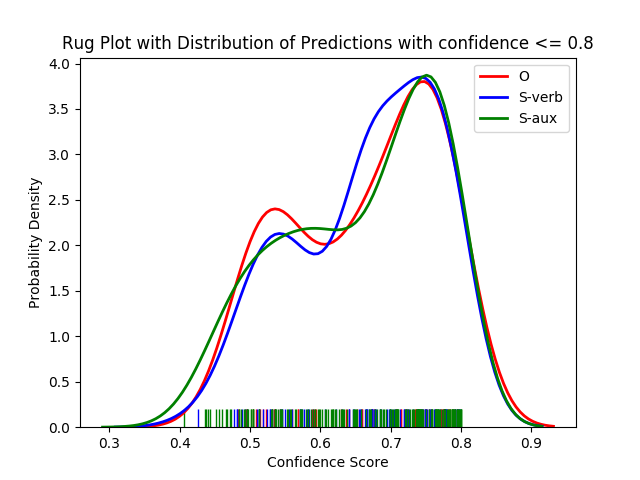
\includegraphics[scale=0.80]{img/aux-verb-distribution.png}
    \caption{Rug plot with Distribution of Predictions with low confidence score}
    \label{fig:auxvsverbsDistribution}
\end{figure}

Having identified instances within each category that have confidence scores within the relevant bound, these instances were manually annotated to see which one of the original annotation or the predicted annotation is correct. We can summarize the entire experiment in the form of algorithm as defined in Algorithm \ref{algo:auxverbAlgo}.

\begin{algorithm}[H]
\caption{Experiment to Identify Mislabelled \texttt{AUX} and \texttt{VERB} tags}
\label{algo:auxverbAlgo}
\begin{algorithmic}[1]
\REQUIRE $data \leftarrow$ UDv2.4 treebank
\STATE Convert $data.train$, $data.test$ and $data.dev$ to IOBES format
\STATE $model.config \leftarrow$ SOTA Classifier Configuration
\STATE $data.complete \leftarrow data.train + data.dev + data.test$
\STATE \COMMENT{The different splits of the data concatenated together}
\STATE $iter.id \leftarrow$ fold of $data.complete$, numbered as $id$
\STATE \COMMENT{Performed 10-fold cross-validation to split $data.complete$}
\STATE $model \leftarrow$ Classifier with configuration as per $model.config$
\FOR {$id$ in \{1, ... , 10\}}
    \STATE $model.id \leftarrow$ $model$ trained on $iter.id.train$ data
    \STATE $model.id.test \leftarrow$ Prediction of $model.id$ on $iter.id.test$ data
\ENDFOR
\STATE $identified.pure \leftarrow$ Original Annotation matches Prediction such that Confidence score \(\leq\) 0.6700
\STATE $identified.cross \leftarrow$ Original Annotation differs from Prediction such that Confidence score \(\geq\) 0.9950
\STATE Manual Annotation of $identified.pure$ and $identified.cross$
\end{algorithmic}
\end{algorithm}

\section{Results}
\label{ssec:auxverbResults}

The associated code for the experiment, alongwith the manually annotated data is available online\footnote{\url{https://github.com/Akshayanti/Masters-Thesis-CUNI-2020/tree/master/AUX-vs-VERB-UDv2.4}}. Given that the experiment is a case of a multi-class classification, the model performance is expressed in form of confusion metrics for each class \verb|AUX|, \verb|VERB| along with the metrics like Precision, Recall, Accuracy, F1 Score.

The metrics corresponding to the best performing model on the original treebank is listed in Table \ref{tab:auxverbBest}. When the models were trained on each of the folds, keeping the architecture of the best model, there was no loss in performance of the trained models (metric considered- micro averaged F1 score). 

% Change to a longtable if needed
\begin{table}[ht]
\centering
    \begin{tabular}{|l|c|c|c|c|}
        \hline
        \textbf{Label} & \textbf{Precision} & \textbf{Recall} & \textbf{Accuracy} & \textbf{F1 Score} \\
        \hline
        \verb|AUX| & 98.89 & 99.50 & 98.40 & 99.19 \\
        \verb|VERB| & 99.32 & 98.87 & 98.20 & 99.09 \\
        \hline
    \end{tabular}
\caption{Metrics of Best Model trained over original \texttt{hi} data}
\label{tab:auxverbBest}
\end{table}

As mentioned in previous section, we focused on the instances of the tagged data with confidence scores in particular bounds. Table \ref{tab:auxverbResults} lists the number of instances that were focused on in each category (as defined in Table \ref{tab:auxverbCategories}). The table also lists the number of instances that were identified as mislabelled, following the annotation procedure.

\newpage
\begin{longtable}{|c|c|c|c|}
\hline 
\multicolumn{1}{|l|}{\textbf{Category}} &
\multicolumn{1}{l|}{\textbf{Focused}} &
\multicolumn{1}{l|}{\textbf{Mislabelled}} &
\multicolumn{1}{l|}{\textbf{Percentage}} \\
\hline 
\endhead
\hline 
\multicolumn{4}{|r|}{{Continued on next page}} \\ 
\hline
\endfoot
\endlastfoot
    \hline
    \label{tab:auxverbResults}
    aux\_TP & 83 & 3 & 3.61 \\
    O\_TP & 25 & 5 & 20.00 \\
    verb\_TP & 45 & 10 & 22.22 \\
    \hline
    aux-O & 10 & 9 & 90.00 \\
    aux-verb & 42 & 23 & 54.76 \\
    verb-O & 20 & 11 & 55.00 \\
    \hline
    \hline
    \textbf{Overall} & 225 & 61 & 27.11 \\
    \hline
\caption{Results of Manual Annotation}
\end{longtable}

\section{Discussion of the Results}
\label{ssec:auxverbDiscussion}

\begin{table}[h]
    \centering
    \begin{tabular}{|l|l|}
        \hline
        \textbf{Metric} & \textbf{Count} \\
        \hline
        Sentences & 16 647 \\
        Words & 351 704 \\
        Tagged \verb|AUX| & 26 030 \\
        Tagged \verb|VERB| & 33 753 \\
        \hline
    \end{tabular}
    \caption{Statistics for \texttt{hi} data}
    \label{tab:auxverbDetails}
\end{table}

Table \ref{tab:auxverbDetails} lists the counts of sentences and the number of \verb|AUX| and \verb|VERB| tags in the entire \verb|hi|-HDTB treebank. Of the total number of tags listed in either category, we are able to focus on just 225 instances where we might be able to identify the problems. Even out of those 225 identified instances, just a bit over 25\% are actually erroneous. 

While hypertuning the best configuration of the classifier, the parameters correspond to the F1 score on how well it fits to the original data. Essentially, the best performing model is biased in the way that it would always try to find a prediction that matches the original annotation. While there is no other way on how to hypertune the model, the experimental results are therefore liable to find comparatively less instances where the confidence score is within the bounds as considered in the experiment. 

Further, the lack of a definable baseline for the attempted solution of the given problem makes it difficult for the current approach to be compared against a benchmark. Considering the lack of benchmark, we can crudely estimate the performance of the experiment by the ratio of the number of errors that were found in the focused cases to the number of instances that were focused on. 

While certain patterns are more reliable than others (the case where predicted output doesn't match the original annotation), the overall performance for the experiment is low as can be attributed to different factors mentioned above. Given the low scout-ability of the error cases in the experiment, the approach used in the experiment is not reliable enough for the process to be automated. % 06 pages on AuxVsVerbs
    \chapter{Future Work Recommendations}
\label{chap:future}

This chapter discusses in brief the other problems that have been recognised within the scope of UD. None of these works mentioned in this chapter have been discussed in the present version of the document. For future researchers interested in tackling more problems with respect to UD, this chapter could be a good point of reference. 

\section{Enhanced Dependencies}
\label{future:enhanced}

Enhanced Dependencies can be understood as an additional layer of annotation of dependencies in UD, which essentially marks added dependencies. Considering some of the restrictions imposed by the regular annotation scheme like a singular head constraint where each node can have only one head, the Enhanced Dependencies aim to cover aspects which can be missed by the regular annotation scheme. However, not all of the languages, or their treebanks have been annotated with the Enhanced Dependencies so far. While the enhanced dependencies have been deemed to be useful in multiple cases (like that of ellipsis, cf. Section \ref{future:ellipsis}), their full potential might not have been realized so far.

In our experiment on \verb|conj_head| (cf. Chapter \ref{chap:conj_head}), we did not work with the problem of conjunction sandwiches. It is very likely that such problems which are difficult to be recognized by the regular dependencies can be searched for rather easily with the Enhanced Dependencies. For example, if Enhanced Dependencies mark all the conjuncts by the \texttt{conj} deprel, regardless of whether they are labelled by the deprel in the regular annotation or not, it would allow searching for the available conjuncts rather easily.

We leave it as an open problem for future research to identify cases which are more difficult to handle with regular dependencies, while trying to use Enhanced Dependencies. As an add-on to the task, it can also be tested if some algorithms mentioned in the research can be improved upon or discarded when Enhanced Dependencies are used.

\section{Ellipsis}
\label{future:ellipsis}

The problem with annotation of Elliptical Structures is big enough to warrant a discussion of its own in UD Annotation Guidelines\footnote{\url{https://universaldependencies.org/u/overview/enhanced-syntax.html\#ellipsis}}\textsuperscript{,}\footnote{\url{https://universaldependencies.org/u/overview/specific-syntax.html\#ellipsis}}. 

\cite{orphan} analyzed the elliptical constructions in UDv2.0 treebanks \citep{UDv2.0} by principally using \verb|orphan| relations\footnote{\url{https://universaldependencies.org/u/dep/orphan.html}} as a way to identify the cases of non-promoted dependents with promoted dependents. While this helps in identifying only a certain number of cases, it fails to identify the cases where the dependents are promoted. 

In Enhanced Dependencies, \verb|orphan| is replaced by placing a null node to indicate the elided token. However, as discussed earlier, Enhanced Dependencies are not available for all languages or even all treebanks in the same language. Thus, the identification and correction of erroneous elliptical constructions remains a problem that needs to be solved within the scope of basic dependency graphs in UD.

\section{\texttt{FalseNonProjective}: Introduction of False Non-Projectivity into the Annotation}
\label{future:nonproj}

While non-projectivity is a characteristic of some languages, and especially more so of certain genres (poetry, for example); the increasing count of non-projective trees has been shown to affect dependency parsing in a negative way. Owing to semi-automatic conversion scheme, a lot of non-projectivities might also be introduced artificially. Thus, it becomes important to not only identify such cases of false non-projectivities (i.e. the cases which should have been marked as projective, but were annotated as non-projective), but also to remove them as it affects the treebank quality in general.

Note that projectivisation or the act of making a non-projective tree as projective is a different research problem. While projectivisation is primarily aimed at trying to create parsers that can parse non-projective trees efficiently (cf. \citep{nivre2005pseudo}, \citep{npparser3}, \citep{npparser1}, \citep{npparser2}, among others) and is therefore a parsing problem; \texttt{FalseNonProjective} is an erroneous non-projectivity introduced in the annotation where the tree is projective, and has no non-projective variants possible.

\section{Function Words and Associated deprels}
\label{sssec:conj_deprels_association}

Conjunctions are identified by two POS tags, viz. \verb|SCONJ|, \verb|CCONJ|. The associated dependency relations for the two POS tags are \verb|mark|, and \verb|cc| respectively. While these are the usually associated dependency relations, the boundary between the two is fuzzy. In the sense, it is possible for a token to be marked by \verb|SCONJ|, and have a \verb|cc| dependency relation (similarly for \verb|CCONJ| and \verb|mark|). Added to this are the cases where the tokens marked by another POS tag can act as conjunctions. Consider the following example from \verb|en|-ParTUT (UDv2.3) and the associated tree in Figure \ref{fig:func_multi}, where \verb|PART| (\textit{to}) acts as a conjunction, and thus the \verb|mark| deprel associated to it.

\begin{example}
\label{example:cc-mark}
Ukraine's constitutional structure is for Ukraine's citizens alone \textbf{to} decide.
\end{example}

\begin{figure}[ht]
    \centering
    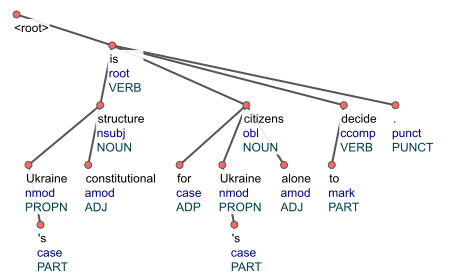
\includegraphics{img/cc-mark.png}
    \caption[Dependency Tree showcasing association of \texttt{PART} with \texttt{mark} deprel]{Dependency Tree for Example \ref{example:cc-mark} showcasing association of \texttt{PART} with \texttt{mark} deprel}
    \label{fig:func_multi}
\end{figure}

Furthermore, both the POS tags in question (\verb|SCONJ|, \verb|CCONJ|) can have other dependency relations attached to them as well. As such, it is difficult (and nonsensical) to limit the deprels for a particular POS tag to occur with a particular deprel (especially in this case). However, there might still be some processes we can observe (and correct). For example, if a particular token occurs more with the \verb|mark| deprel, but is consistently labelled as \verb|CCONJ|, the annotation should be taken a closer look at, and a possible disparity identified.

\section{\texttt{auxHead}: Auxiliary as Head of Dependency}
\label{future:auxHead}

In the discussion of this problem, we refer to the case when an auxiliary (marked by either of \verb|AUX| or \verb|aux|) is treated as the head of a dependency relation. Although allowed in certain cases, the auxiliary should not be marked as the dependency head in general sense. Consider the following example in Figure \ref{fig:aux-head-example}, taken directly from \cite{alzetta2017dangerous}. The token of interest is marked in bold.

\begin{example}
\textbf{ }\\
\textbf{Text (\texttt{it}):} Per noi \textbf{\`e} stato sufficiente che andassero via\\
\textbf{Lit.:} For us it-has been enough that they-went away\\
\end{example}
    
\begin{figure}[H]
    \centering
    \begin{subfigure}{.45\textwidth}
  \centering
  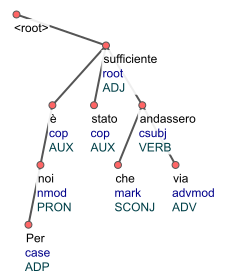
\includegraphics[scale=0.90]{img/before-aux.png}
  \caption{Original (Incorrect) Annotation}
  \label{fig:aux-head-skewed}
  \end{subfigure}
  \begin{subfigure}{.45\textwidth}
  \centering
  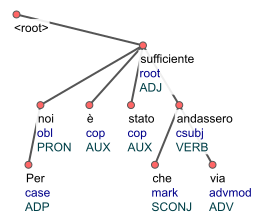
\includegraphics[scale=0.90]{img/after-aux.png}
  \caption{Corrected Annotation}
  \label{fig:aux-head-corrected}
  \end{subfigure}
    \caption[Example tree from \cite{alzetta2017dangerous} showcasing \texttt{auxHead} error type]{Example tree from \cite{alzetta2017dangerous} showcasing \texttt{auxHead} error type. In the original example, \textbf{noi} (us) was annotated as a dependent of both  \textbf{Per} (for), and \textbf{\`e} (has-been). Under UD representation, there can not be more than one head for any given node in regular annotation. As such, we believe it was a typo in the publication and not in their data. In this figure, we show the corrected dependencies.}
    \label{fig:aux-head-example}
\end{figure}
    
In the figure, notice how the originally incorrect annotation has \textit{\`e} (has-been) with POS \verb|AUX| serving as a dependency head. \citeauthor{alzetta2017dangerous} notice that this particular error, classified as a head identification error, contributes to around 13 \% of the total discovered erroneous instances. Since it is difficult to separate and identify the instances marked correctly as \verb|AUX| (cf. Chapter \ref{chap:failures} for the experiment on attempt at differentiation between \verb|AUX| and \verb|VERB|  tags), the attempt at the solution for this problem was not worked at.

\section{\texttt{nmod4obl}: Confusion of \texttt{nmod} and \texttt{obl} Relations}
\label{sec:probnmod4obl}

In UDv1, \verb|nmod| relation was used for nominals modifying either predicates or other nominals. Following a change in guidelines in v2, the deprel was restricted to modifying nominals. Furthermore, a new relation \verb|obl| (oblique) was introduced for oblique dependents of predicates.

To put it simply, this conversion implied the following in an equation format, where \(\verb|x|_{vi}\) refers to the dependency relation \(\verb|x|\) as used in version \(i\) of UD treebanks:

\begin{equation*}
    \boxed{\texttt{nmod}_{v1} = \texttt{nmod}_{v2} \cup \texttt{obl}}
\end{equation*}

Depending on the parent node, the relations were modified as follows:

\begin{enumerate}
    \item If the parent node was a verb, the deprel was changed from \texttt{nmod} to \texttt{obl}.
    \item If the parent was a nominal predicate, the deprel could be either of \texttt{nmod} or \texttt{obl}, depending on if only the nominal was being modified, or the whole clause was being modified.
    \item If the parent was a nominal, but not a nominal predicate, there was no change in the deprel.
    \item If the parent was an adjective or an adverb, the deprel would be changed to \texttt{obl}, based on additional conditions.
    \item In case none of the above conditions held true, the instance would deserve individual treatment.
\end{enumerate}

The change in definition from UDv1 to UDv2 was the primary cause of the error, as identified in \cite{alzetta2017dangerous}. In the same work, the authors note that this error contributes to around 7 \% of total discovered errors in the newspaper section of the Italian UD Treebank (IUDT). In the work, the authors attribute this error pattern to annotation inconsistency internal to the treebank. Although a significantly important error, this is not covered in the scope of the current research. Nonetheless, this is an important error that should be taken care of in future.

\section{Punctuation}

The UD Annotation guidelines on punctuation are simple and straightforward\footnote{\url{https://universaldependencies.org/u/overview/specific-syntax.html\#punctuation}}. There are discrepancies when it comes to implementation of the guidelines. Some of them are listed as below:

\begin{enumerate}
    \item It is difficult to identify the next conjunct in case of missing \verb|CCONJ| and \verb|SCONJ| tags as in case of asyndetic coordination. In such cases, the information about the next conjunct should be deduced semantically in most cases. We saw a similar case in Section \ref{sec:conj-sand} (Example \ref{examp:nonconj} and Figure \ref{fig:nonconj}) where the next conjunct is not clear, owing to other (more suitable) deprel(s) being used in place of \verb|conj| deprel.
    \item Re-attachment of a punctuation node is a problem that goes with the previous instance since it's not always clear at what level the punctuation must attach to.
    \item For paired and nested punctuation, different languages use different sets of nested punctuation pairs, specifically with respect to quotation marks. As such, the treatment of paired punctuation pairs needs to be handled in a language-specific manner.
\end{enumerate}

The \verb|fixpunct.py| block in Udapi-python \citep{udapi} tries to take care of significant number of edge cases in different UD treebanks. However, a more concrete solution is needed for the problems aforementioned.

\section{Unspecified Dependencies - \texttt{dep} deprel}

According to the UD definition of \verb|dep| deprel\footnote{\url{https://universaldependencies.org/u/dep/dep.html}}, the deprel is reserved for cases when a more precise relation cannot be found. This can be either owing to the sentence splitting in treebanks of some languages, or owing to the limitation in parsing software. Nonetheless, the relation should be avoided as much as possible.

Noticing that some treebanks follow sentence splits where the parts of sentences might be labelled as different sentences (as in the example of a list), the deprel in question is more liable to be used in such instances. However, looking at the data in UDv2.4, some languages have more than 1\% of the tokens marked with such relation (Examples being \verb|ko|, \verb|ur|, \verb|ja|-BCCWJ, \verb|it|-PoSTWITA, \verb|hi|-HDTB, \verb|gl|-CTG, \verb|cs|-PDT, among others). While these might be all true positives in other languages, a significantly higher count of \verb|dep| is more troublesome and is less likely to be all true positives in such cases.

An experiment can be performed on such instances where the data without any \verb|dep| deprel is used as a training set to parse the instances with the deprel in question and then the results verified. Nonetheless, the cases of tokens marked with deprel in question need to be reduced in some languages. As such, we leave it as a problem for future researchers to tackle. % 06 pages on Future Recommendations
    \chapter*{Conclusion}
\addcontentsline{toc}{chapter}{Conclusion}

Although the official title of the research seeks to deal with inconsistencies, this work bounces between error detection and correction, and inconsistency detection and correction. We started with an introduction of an evaluation method to check the POS annotation quality of treebanks in a language, followed by an inspection of an inconsistency detection tool (LISCA) and if it can be extended to be used for low resource data. We also tried to correct the problematic instances identified by researchers before us. While some of the attempts at the solutions have been successful, others still need refinement and additional work to complete them, owing to their time requirements.

As the cost of storage falls lower, the size of the treebanks would increase. Essentially, at one point it might be impossible for human annotators to be part of the error-identification and error-correction process for the entire treebank. The current work is primarily aimed at finding the methods that don't need human annotators in the pipeline, and can be relied upon to fix the errors across different languages in a reliable manner. The research has been in some aspect successful at that front.

One major advantage of an iterative process, with respect to UD treebanks, is how individual error types can be focused on in each iteration. With the UD validator (cf. Level 5 checks in \verb|validate.py|\footnote{\url{https://github.com/UniversalDependencies/tools}} file) identifying and notifying the development teams of the individual errors, the process no longer suffers from a cold start problem. There is a high chance that with upcoming iterations, more and more of the experiments discussed in the document would be rendered obsolete for new treebanks, but they are still necessary to fix the issues in the present treebanks.

It is important to note here that the different problems listed in this thesis document rarely occur in isolation. More often than not, many of the problems are intertwined with each other, resulting in error propagation. Having said that, the corrections are also propagated in a similar fashion, whereby finding and correcting the right error solves multiple intertwined issues at the same time. Consider the example of experiment on \texttt{conj\_head} (in Chapter \ref{chap:conj_head}). Correction of this error instance in the specific case of \verb|eu| also corrected the case of falsely annotated non-projectivities in the trees.

Of the problems mentioned in the chapter titled `Future Work Recommendations' (Chapter \ref{chap:future}), there are some that were not worked on at all in the current research and are left for future researchers (For example, \texttt{nmod4obl} in Section  \ref{sec:probnmod4obl}). Additionally, some other problems are still being worked on, and thus do not fall into the scope of the current thesis document (For example, \texttt{FalseNonProjective} and \texttt{auxHead} in Sections \ref{future:nonproj} and \ref{future:auxHead} respectively).

The author hopes that the future researchers will be able to tackle the problems as listed in this thesis in a greater capacity, and improve upon the methods already discussed in this research wherever possible. % 01 pages on Conclusions
% \chapter{Experiment 1: Intra-Language Inter-Treebank Harmony}
\label{chap:harmony}

\cite{alonso2016universal} note that if the two treebanks from the same language are as similar as possible, the differences in parsing accuracy (training parser on one of the treebanks, and using it to parse the other language) would be due to differences in dataset size, and domain change; but not due to differences in dependency convention.

\cite{klcpos3} show that KL-Divergence score of POS trigrams can be effectively used for source selection for POS Tagging in a delexicalised cross-language model transfer scenario. In their approach, they are able to select effectively not just a singular source, but also for source-weighting in multi-source transfer. Computing the KL-Divergence on POS trigrams, they call the measure as \(KL_{cpos^3}\), defined as follows:

\theoremstyle{definition}
\begin{definition}
\label{def:klcpos3}
\begin{equation}
\label{eqn:klcpos3}
    KL_{cpos^3}(tgt, src) = \sum_{\forall cpos^3 \in tgt}^{}f_{tgt}(cpos^3)\cdot\log\dfrac{f_{tgt}(cpos^3)}{f_{src}(cpos^3)}
\end{equation}
where \(cpos^3\) is a coarse POS tag trigram, and \\
\begin{equation}
\label{eqn:cpos}
    f(cpos^3) = f(cpos_{i-1}, cpos_{i}, cpos_{i+1}) = \frac{count(cpos_{i-1}, cpos_{i}, cpos_{i+1})}{\sum_{\forall cpos_{a,b,c}}{count(cpos_{a}, cpos_{b}, cpos_{c})}}
\end{equation}
with \(count_{src}(cpos^3) = 1\) for each unseen trigram.
\end{definition}

Intuitively, treebanks of the same language should be a better fit for single-source transfer than a treebank from another language, and so \(KL_{cpos^3}\) for a single-source transfer can be considered as a good benchmark for deciding this. However, \(KL_{cpos^3}\) is a variant of KL-Divergence, and thus is asymmetric. Therefore, we should rely on a metric that can calculate the divergence of the treebanks from each other, in both directions.

Combining the above two observations, we can arrive at a definition of treebank harmony.

\theoremstyle{definition}
\begin{definition}
\label{def:harmony}
Given two treebanks \(A\) and \(B\), we say the treebanks are in harmony with (or, are harmonious to) each other, iff
\begin{enumerate}
    \item The difference in labelled attachment scores (LAS) when trained on one treebank and tested on another, denoted by \(\theta_{LAS}\), is less than or equal to a given threshold \(\theta_1\). \\
    Mathematically, it can be represented as:
    \begin{equation}
    \label{eq:deprel_harmony}
        \theta_{LAS} = \vert {LAS}_{x,x} - {LAS}_{y,x} \vert \leq \theta_1 \hspace{5mm} \quad \forall [x, y \in \{A,B\}]
    \end{equation}
    where \(LAS_{P,Q}\) indicates LAS when trained on \(P\) and tested on \(Q\).
    \item The difference in \(KL_{cpos^3}\) scores of the treebanks calculated in both directions, denoted by \(\theta_{POS}\), is less than or equal to a given threshold \(\theta_2\). \\
    Mathematically, it can be represented as:
    \begin{equation}
    \label{eq:pos_harmony}
        \theta_{POS} = KL_{cpos^3}(A,B) + KL_{cpos^3}(B,A) \leq \theta_2
    \end{equation}
    where \(KL_{cpos^3}(P,Q)\) indicates \(KL_{cpos^3}\) score of \(Q\) as an estimator for \(P\).
\end{enumerate}

Mathematically, we denote two harmonious treebanks \(A,B\) as \(A \doteq B\) over (\(\theta_1, \theta_2\)). The relation of harmony is reflexive, symmetric, but not transitive.
\end{definition}

As mentioned earlier, there exist up to 6 different treebanks (not including PUD) for a given language. More often than not, the treebanks cover different domains, and are of different sizes. As such, it becomes an important criteria to determine the appropriate values for \(\theta_{1}\) and \(\theta_{2}\). If the values are too large, we run the risk of saying the treebanks are harmonious even when they might not be. Also, if the values are too small, we could be overlooking at the effect of domain change and dataset size, to mistake the two treebanks as being non-harmonious to each other.

\section{Dataset}
\label{sec:dataset_harmony}

Before we start tuning the hyper-parameters, we need to define our dataset. This experiment was conducted entirely on UDv2.5 data, without exceptions. To minimize the effect of dataset size disparity, we remove from consideration all the treebanks which are missing train data, as listed in Appendix \ref{app:treebank_data}. From these treebanks, we remove only the ones which do not contain any train data whatsoever.

Furthermore, there are treebanks which have data in the format where it needs to be fetched from another corpus and is not readily available for usage. We discard such treebanks as well from the consideration. Thus, the effective dataset for this entire experiment can be seen in Table \ref{tab:dataset_harmony} as follows:

\begin{table}[H]
    \centering
    \begin{tabular}{|l|c|l|}
    \hline
    Language & Count & Treebank Names \\
    \hline \hline
    cs & 4 & CAC, CLTT, FicTree, PDT \\
    en & 4 & EWT, GUM, LinES, ParTUT \\
    es & 2 & AnCora, GSD \\
    et & 2 & EDT, EWT \\
    fi & 2 & FTB, TDT \\
    fr & 3 & GSD, ParTUT, Sequoia \\
    gl & 2 & CTG, TreeGal \\
    grc & 2 & Perseus, PROIEL \\
    it & 4 & ISDT, ParTUT, PoSTWITA, VIT \\
    ko & 2 & GSD, Kaist \\
    la & 3 & ITTB, Perseus, PROIEL \\
    lt & 2 & ALKSNIS, HSE \\
    nl & 2 & Alpino, LassySmall \\
    no & 3 & Bokmaal, Nynorsk, NynorskLIA \\
    pl & 2 & LFG, PDB \\
    pt & 2 & Bosque, GSD \\
    ro & 2 & Nonstandard, RRT \\
    ru & 3 & GSD, SynTagRus, Taiga \\
    sl & 2 & SSJ, SST \\
    sv & 2 & LinES, Talbanken \\
    \hline
    \end{tabular}
    \caption{Dataset for the Experiment on Harmony Between Treebanks, UDv2.4}
    \label{tab:dataset_harmony}
\end{table}
% % \subsection{Other Factors}
% \label{ssec:others_theta2}

% We took into account the two major factors that causes a dip in parser performance. However, there are a few other factors that also affect the parser performance. We discuss some of those factors in this subsection, without performing any experiments on them. Thus, we don not account for these features in our definition of harmony of treebanks, as we argue that these features should be corrected in treebanks (wherever necessary, and possible), rather than being accounted for.

% We do not account anywhere for genre-specific vocabulary in any of the cases, since \cite{alonso2016universal} and \cite{RussianTreebanks} prove in their experiments that LAS scores are not affected by genre/topic-specific vocabulary.

% \subsubsection{Very Long Sentences}

% We define very long sentences as the sentences with more than the average number of tokens (defined on a per-language basis). As the sentence length increases, the distance of the nodes from the root of the sentence also increases. \cite{collins} showed how the distance between a token and the sentence root affects parser performance for trees. We can safely extrapolate on that information to extend it to the case of dependency parsing as well.

% As the number of very long sentences increase in the treebank, the parser performance on the individual sentences decreases, and therefore the total score on the entire treebank as well. While it might not always be possible to get rid of such very long sentences from the treebank, care should be taken to keep the count of such sentences as minimal as possible, or a separate parser could be trained on such sentences separately.

% \subsubsection{Non-Projective Structures}

% The presence of projective structures has been known to affect the parsing quality. The greater the difference in number of non-projective structures, the greater the difference in the parser performance. Minimising the number of non-projective structures in the treebanks is a definite way to reduce the degree by which the treebanks differ.

% \subsubsection{Differences in Annotation Strategies}

% In different treebanks from the same language, there might not be agreements in the annotation scheme. As \cite{RussianTreebanks} note, the difference in annotation of \textrussian{бы} (\textit{by}; would) in \verb|ru|-SynTagRus and \verb|ru|-Taiga as an auxillary in the different treebanks causes the parser trained on \verb|ru|-SynTagRus to be able to predict only 5\% of functional relations in \verb|ru|-Taiga. Other annotation inconsistencies, like those of tokenisation of multi-word entities (MWEs), parataxis, \verb|SYM| vs \verb|PUNCT|, etc. also cause a dip in parser performance. Such inconsistencies are often a result of individual team's decision on annotation strategies differing from each other.

% A correction on this aspect requires a more coherent dialogue between the different teams responsible for development of different treebanks, and should be encouraged. While it might not always be possible to catch these differences by an automatic tool also because we need to identify the areas where the annotation might be inconsistent between treebanks; the concept of variation nuclei \citep{boyd} can be used to some extent.

% \subsubsection{Other Incorrigible Factors}

% Apart from the above mentioned factors, the treebanks on the same language can also be influenced by the regional differences in the language. Consider the case of \verb|en|, and with reference to the difference in the spelling distinctions between American English and British English. In case of a lexicalized parsing scenario, the differences in spelling can make differences on how the parser reacts to different tokens. Another notable example is with respect to Spanish spoken in Spain, and the variation(s) of it with respect to Spanish as spoken in Latin America.

% \subsection{Brief Discussion on the metric}

% The architecture of a parser used for calculating \(\theta_{1}\) metric also would essentially change the variation of the scores, based on genres or on size. For example, the size-based disparity scores are in line with \cite{velldal-etal-2017-joint} where they report the similar patterns with respect to size variations. It might be an interesting study to extend the study based on this to different architectures and study the variation of scores in cases of genre-distribution as well as size-disparity.

\newpage

% \section{Combining Optimized Values}

In our experiments, we tried to optimize the two parameters \(\theta_{1}\) and \(\theta_{2}\) based on size and genre variations, by considering only one at a time. As mentioned earlier, this is not always possible since the premise of the genre-distribution based study is the isolation of individual genres. The isolation is not always possible. Also, while some genres are intuitively extremely different (like wiki data and internet slangs), some others are not very much so (like wikipedia and nonfiction). In case of the experiment for \(\theta_{POS}\) based on genre distribution, the different distribution of UPOS in a different language might affect the scores for the gathered limits to be deemed useless.

Also is important to note that the genre-distribution and size-disparity can occur together. In the sense, there can be different number of genres, and with each genre having a different size in the treebanks being compared. In such a case, the metric would need to be compared for size per genre, on basis of genre-distribution and finally, the overall size of the treebank.

While the metric reported in this experiment is far from perfect, it gives something to start comparing the data in different treebanks. We discussed the metric for calculating POS distribution, as well as LAS scores. It is not possible to identify and localize the source of errors using the metric, but it narrows the search space on where to look for. This, of course, only holds true if the genre distribution can be identified, and size composition of different genres identified.

It would be an interesting study for future to learn if the effects of genre addition/removal are uniform across all genres, or are certain genre pairs more accommodating to each other (in the sense of less variance in LAS scores between them).

% \section{Further Discussion}
% \chapter{Experiment4: Mining False Non-Projective Structures}
\label{chap:nonproj}

\section{Observations About Problem Statement}
\subsection{Projectivization vs False Non-Projectivity}

Projectivization can best be defined as making a non-projective structure artificially projective. This could be for the sake of training a parser, or to form a phrase-based constituency tree, among others. \cite{nivre2005pseudo} discuss the projectivization procedure for a non-projective edge using a process called edge lift. In the process, once a non-projective edge is detected, it is re-attached to the grandparent node as per the original attachment. The authors also define a minimal projective transformation to remove non-projective edges from a tree in an iterative manner. To do so, the algorithm starts with the node that has the least distance between the head and the dependent, and then performs lift operation on it, repeating the process until the entire tree is projectivized. The authors use this approach to find an optimal parser for parsing non-projectivities in the languages. A udapy-python block on the method of \citeauthor{nivre2005pseudo} is also under development\footnote{\url{https://github.com/udapi/udapi-python/tree/master/udapi/block/transform}} at the time of writing this document.

While there have been several publications on how to develop parsers that can parse non-projective trees efficiently (\citep{npparser1}, \citep{npparser2}, \citep{npparser3}, among others), there are also multiple works in an attempt to understand the linguistic features that cause non-projectivities (\citep{mannem2009insights}, \citep{mambriniNonProj},
\citep{npprojvalency}, among others). The need for automatic error-correction methods for treebanks was realised early on, thanks to \cite{boyd}. Since then, the focus of such techniques for dependency treebanks has been limited to either determining the direction of association of edges, determining right candidate node for association (also intersects with dependency parsing), or determining the correct association between the nodes. While a search for false non-projective structures would also employ all of the above, this is the first work that focuses on the particular problem of finding false non-projective structures.

\cite{mannem2009insights} inspect the causes of non-projectivity in Hyderabad Dependency Treebank\footnote{Later adapted into UD as \texttt{hi}-hdtb treebank} (HyDT) for \verb|hi| where they define the notion of rigidity of a non-projective structure as the possibility of reordering the construction without losing on the meaning of a sentence (not taking into consideration the discourse and topic-focus). The authors look at major causes of non-projectivities in the treebank, and classify each of the cause as rigid/non-rigid based on if it is possible to remove non-projectivity from the structure through reordering. Out of the total number of non-projective structures in the treebank, only around a 20\% of them could be classified as rigid structures, which couldn't be projectivized. The authors rely on their knowledge of the language to classify the underlying causal linguistic phenomenon (of non-projectivity) as rigid/non-rigid, without offering any (data driven) rules to determine the rigidity of a structure. The authors also define the notion of \textit{naturalness} of a projectivized construction, based on if the speakers of language would prefer a projective or non-projective structure. Again, this is also not defined in an empirical manner, but is open to subjectivity of the speaker of the language. Although the definition of rigidity can come handy in context of free word-order languages, it is not a metric that can be employed to all languages universally. Extending definitions given by \citeauthor{mannem2009insights} and based on their classification, we would like to differentiate between a few different kinds of non-projective structures as below, while still going by the definition of \textit{rigidity} and \textit{natural}-ness as given by the authors.

\begin{enumerate}
    \item Not rigid, and \textbf{does not} require reordering for natural projectivity
    \item Not rigid, and \textbf{does} require reordering for natural projectivity
    \item Not rigid, and no natural projectivity possible
    \item Rigid, with natural projectivity possible
    \item Rigid, and no natural projectivity possible
\end{enumerate}

Given that we are not interested in reordering the nodes of a tree in a given treebank, the second case as mentioned above does not warrant consideration in the present research. For the exact same reason, we can combine remaining cases to get the following two cases, referred to as condensed cases henceforth:

\begin{enumerate}
    \item \textbf{Natural Projectivity Possible}: A given edge can occur non-projectively, as well as projectively. A very common example of this can be seen in poetry, or in elliptical constructions where the choice of construction can make an edge projective or non-projective.
    \item \textbf{Natural Projectivity Not Possible}: There are a few constructions that seem to always introduce non-projectivity. In \verb|hi|, the tendency is exhibited by token \texthindi{कि} (\textit{ki}; that) as pointed out by \cite{mannem2009insights}.
    
\end{enumerate}

Different treebanks in UD do not annotate the multiple possible structures of a given sentence, but rather the most frequently used one. Therefore, a given sentence (or a sequence of tokens contained therein) can be categorised in either of the two condensed cases. In this experiment, we seek to identify the cases of the first kind where an edge has been annotated as non-projective, when a projective edge is more likely. Going the reverse way, we also want to identify the cases where a given edge in second case has been annotated as a projective edge. To do so, we use the concept of variation nuclei as used in \cite{boyd}. We have not yet defined the \textit{natural}-ness of a construction so far, in terms of data-driven approach. We do not go over the concept here, but elaborate on it alongwith the discussion of variation nuclei in Section \ref{sec:variation}.

\subsection{Terms Related to Non-Projectivity}

In a directed edge \(i \rightarrow j\), we refer to \(i\) as head, and \(j\) as dependent. Unless mentioned otherwise, we refer to directed edges, with the ordered pair \((i, j)\) denoting \(i \rightarrow j\). We refer to the subtree, rooted at node \(i\) as \(Subtree(i)\). To specify that node \(i\) precedes node \(j\) in tree, we denote it in the form of \(i < j\). A node \(x\) is said to be in gap of non-projective edge if \((i,j)\) if \(x \in (i, j) \And x \notin Subtree(i)\). Alternatively, the node \(x\) is said to belong to gap of \((i, j)\), denoted as \(x \in Gap(i, j)\).

Edge degree is defined as the number of nodes in a tree \(T\) that are in gap. The edge-degree of a tree is defined as the maximum edge-degree from the individual edge's edge-degree. While this is based on a per-edge basis, a gap degree is defined as the number of times a non-projective edge's gap is broken. A very trivial way of calculating gap degree of an edge (\(i, j\)) is to iterate through the nodes in order. Let us say, we have node \(x \in (i, j)\). If \(x\) alongwith its immediate neighbours are all in \(Subtree(i)\) or if none of them is, the gap is not broken. Every time the condition is not met, the gap is said to be broken. The gap degree of an edge is the number of times the gap is broken. Similar to the definition of edge-degree of a tree, gap degree of a tree is the maximum gap degree among all edges therein.


\subsection{Genre Association with Non-Projectivity}



The rest of the chapter is organised as follows. Section \ref{sec:nonproj_dataset} talks about the used dataset for the experiment. We split the analysis of the data in two parts, analysing the non-mild non-projective structures in Section \ref{sec:nonmildnonproj}, and then discussing the concept of variation nuclei and the selection (and querying process) of variation nuclei in mild non-projective structures in Section \ref{sec:variation}. We continue with an evaluation of the findings of the experiments in Section \ref{sec:nonprojeval}. Section \ref{sec:nonprojconclude} concludes.

\section{Dataset}
\label{sec:nonproj_dataset}

The experiment was started on UDv2.3, and eventually brought over to UDv2.4. The experiment(s) on non-projective structures in a treebank were tried over an extended period of time, and as the newer versions of UD were released, the dataset for the experiment changed. The presented version of the experiments was conducted over UDv2.5 \citep{UDv2.5}. As with other experiments that changed datasets in the chronology of the research, the number of problematic cases have diminished over the newer versions of UD. Nonetheless, the problem of identifying the incorrect cases of non-projectivity in a treebank is still relevant, especially in case of treebank(s) of languages where non-projectivity is already established as a common phenomenon\footnote{As mentioned earlier, there exists an association between the genre of the text and the counts of non-projective structures therein. Although we do not discard that association, in this context we refer to the languages where the probability of finding non-projectivities in high, regardless of the genre.} (\cite{mambriniNonProj}, \cite{indic-riyaz}, \cite{Havelka}).

The \verb|fixpunct| block\footnote{\url{https://github.com/udapi/udapi-python/blob/master/udapi/block/ud/fixpunct.py}} of udapi-Python \citep{udapi} attempts to rehang the punctuation nodes. This also takes care of the punctuation nodes that cause non-projectivity, or are attached non-projectively. Since the procedure of lifting the punctuation nodes is not deterministic, there are times when the udapi block makes the situation worse, by introducing non-projectivities in the given data\footnote{One such example can be seen in case of \texttt{cs}\_pdt in Table \ref{tab:treatment-results} where the number of non-projective edges is increased, post application of the udapi block on the treebank}.

UDv2.5 contains 157 treebanks in 90 languages. Of those treebanks, we disregarded PUD treebanks entirely from the consideration, owing to their small size (1000 sentences). In the remaining treebanks, there exist considerable number of non-projectivities induced due to punctuation (cf. Section \ref{ssec:punct-nonproj}). The \verb|fixpunct| block is applied on these treebanks to eliminate cases of punctuation induced non-projectivity.

Having treated the treebanks with udapi-python block, there were 2 categories of treebanks that were chosen as experimental data. The first category, hereafter referred to as \texttt{working treebanks}, contains top 10 treebanks (ranked in order of percentage composition of non-projective trees) which satisfy the following conditions:
\begin{enumerate}
    \item Total number of trees \(\geq 10,000\)
    \item Number of non-projective trees \(\geq 10\% \cdot \) Total number of trees
\end{enumerate}
The second category is hereafter referred to as \texttt{support treebanks}. This category consists of the treebanks that provide added instances of data for treebanks found in \texttt{working treebanks}. For a treebank \(T_{w} \in\) \texttt{working treebanks}, a candidate treebank \(T_{c}\) can be included in the list of \texttt{support treebanks} if it satisfies the following conditions:
\begin{enumerate}
    \item Language of \(T_{w} = \) Language of \(T_{c}\)
    \item Total number of trees in \(T_{c} \geq 5,000\)
    \item Number of non-projective trees in \(T_{c} \geq 5\% \cdot \) Total number of trees in \(T_{c}\)
    \item Genre composition of \(T_{c} \subseteq \) Genre composition of \(T_{w}\)
\end{enumerate}

Having considered the conditions for each category, we get a list of treebanks as can be seen in Table \ref{tab:nonproj_dataset}. The table also shows the counts of trees which fail the relaxations to the conditions of non-projectivity as well (cf. Section \ref{ssec:nonproj-relaxations}). The two categories of treebanks, viz. \texttt{working treebanks} and \texttt{support treebanks} are separated by a horizontal line in the table. In all instances where the two categories are maintained separate, the results of the treebanks shall be included in the same manner, with a horizontal line in between. Table \ref{tab:gap_degrees} and Table \ref{tab:edge_degrees} show the gap degree and edge degree statistics respectively for the experimental data. The effect of application of udapi-python block can be seen in Table \ref{tab:treatment-results} where the counts of non-projective edges are listed for the treebanks in the experimental data. Table \ref{tab:allnpudv2.5} shows the counts of all non-projective structures, and their relaxations in UDv2.5. 

\begin{table}[H]
    \centering
    \begin{tabular}{|l|c|c|c|c|c|c|c|}
    \hline
    \multirow{2}{*}{\textbf{Treebank}} &
    \multirow{2}{*}{\textbf{\# Trees}} & 
    \multicolumn{2}{c|}{\textbf{Non-Proj.}} & 
    \multicolumn{2}{c|}{\textbf{Non-Planar}} & 
    \multicolumn{2}{c|}{\textbf{Ill-Nested}} \\
    & & Trees & \% & Trees & \% & Trees & \% \\
    \hline
    \hline
    \texttt{grc}\_perseus & 13 919 & 8 683 & 62.38 & 1 098 & 7.89 & 126 & 0.91\\
    \texttt{grc}\_proiel & 17 080 & 6 409 & 37.52 & 392 & 2.30 & 38 & 0.22\\
    \texttt{la}\_ittb & 21 011 & 7 680 & 36.55 & 338 & 1.61 & 35 & 0.17\\
    \texttt{la}\_proiel & 18 411 & 5 227 & 28.39 & 448 & 2.43 & 38 & 0.21\\
    \texttt{ko}\_kaist & 27 363 & 5 875 & 21.47 & 83 & 0.30 & 0 & 0\\
    \texttt{fro}\_srcmf & 17 678 & 2 726 & 15.42 & 290 & 1.64 & 82 & 0.46\\
    \texttt{orv}\_torot & 16 944 & 2 575 & 15.20 & 71 & 0.42 & 4 & 0.02\\
    \texttt{nl}\_alpino & 13 578 & 1 953 & 14.38 & 128 & 0.94 & 0 & 0\\
    \texttt{hi}\_hdtb & 16 647 & 2 264 & 13.60 & 116 & 0.70 & 13 & 0.08\\
    \texttt{cs}\_cac & 24 709 & 3 143 & 12.72 & 50 & 0.20 & 14 & 0.06\\
    \hline
    \texttt{cs}\_pdt & 87 913 & 10 145 & 11.54 & 159 & 0.18 & 47 & 0.05\\
    \texttt{nl}\_lassysmall & 7 338 & 446 & 6.08 & 25 & 0.34 & 1 & 0.01\\
    \hline
    \end{tabular}
    \caption{Non-Projectivity and Relaxations in Experimental Data}\% is calculated on the total number of trees (\# Trees)
    \label{tab:nonproj_dataset}
\end{table}

\begin{table}[H]
    \centering
    \begin{tabular}{|l|c|c|c|c|c|}
    \hline
    \multirow{2}{*}{\textbf{Treebank}} &
    \multicolumn{5}{c|}{\textbf{Gap Degree}} \\
    & gd0 & gd1 & gd2 & gd3 & gd4+\\
    \hline
    \hline
    \texttt{grc}\_perseus & 45.57 & 50.59 & 3.72 & 0.12 & - \\
    \texttt{grc}\_proiel & 66.70 & 31.18 & 2.04 & 0.08 & <0.01\\
    \texttt{la}\_ittb & 68.74 & 30.20 & 1.06 & <0.01 & - \\
    \texttt{la}\_proiel & 77.31 & 21.70 & 0.93 & 0.05 & <0.01 \\
    \texttt{ko}\_kaist & 84.54 & 15.36 & 0.10 & - & - \\
    \texttt{fro}\_srcmf & 89.11 & 10.58 & 0.29 & 0.02 & <0.01 \\
    \texttt{orv}\_torot & 87.94 & 11.77 & 0.29 & <0.01 & - \\
    \texttt{nl}\_alpino & 90.48 & 9.31 & 0.20 & - & <0.01 \\
    \texttt{hi}\_hdtb & 89.49 & 10.19 & 0.28 & 0.04 & <0.01 \\
    \texttt{cs}\_cac & 92.41 & 7.52 & 0.07 & - & - \\
    \hline
    \texttt{cs}\_pdt & 92.81 & 7.06 & 0.12 & <0.01 & <0.01 \\
    \texttt{nl}\_lassysmall & 95.97 & 3.95 & 0.08 & - & - \\
    \hline
    \end{tabular}
    \caption{Gap Degrees (in \%) in Experimental Data}\% is calculated on the total number of edges
    \label{tab:gap_degrees}
\end{table}

\begin{table}[H]
    \centering
    \begin{tabular}{|l|c|c|c|c|c|}
    \hline
    \multirow{2}{*}{\textbf{Treebank}} &
    \multicolumn{5}{c|}{\textbf{Edge Degree}} \\
    & ed0 & ed1 & ed2 & ed3 & ed4+\\
    \hline
    \hline
    \texttt{grc}\_perseus & 37.62 & 35.70 & 12.37 & 6.19 & 8.12\\
    \texttt{grc}\_proiel & 62.48 & 23.58 & 6.74 & 3.06 & 4.14\\
    \texttt{la}\_ittb & 63.45 & 25.47 & 4.63 & 2.52 & 3.93\\
    \texttt{la}\_proiel & 71.61 & 17.33 & 5.04 & 2.60 & 3.41\\
    \texttt{ko}\_kaist & 78.53 & 6.02 & 3.35 & 2.48 & 9.61\\
    \texttt{fro}\_srcmf & 84.58 & 5.39 & 4.18 & 2.40 & 3.45\\
    \texttt{orv}\_torot & 84.80 & 9.84 & 2.67 & 1.29 & 1.39\\
    \texttt{nl}\_alpino & 85.62 & 6.47 & 3.87 & 1.86 & 2.18\\
    \texttt{hi}\_hdtb & 86.4 & 4.05 & 3.07 & 2.62 & 3.85\\
    \texttt{cs}\_cac & 87.28 & 6.58 & 3.12 & 1.33 & 1.68\\
    \hline
    \texttt{cs}\_pdt & 88.46 & 5.41 & 2.82 & 1.26 & 2.05\\
    \texttt{nl}\_lassysmall & 93.92 & 2.89 & 1.46 & 0.76 & 0.97\\
    \hline
    \end{tabular}
    \caption{Edge Degrees (in \%) in Experimental Data}\% is calculated on the total number of edges
    \label{tab:edge_degrees}
\end{table}

\begin{table}[H]
    \centering
    \begin{tabular}{|l|c|r|c|r|c|}
    \hline
    \multirow{2}{*}{\textbf{Treebank}} &
      \multirow{2}{*}{\textbf{\# Edges}} &
      \multicolumn{2}{c|}{\textbf{Non-Proj. Edges\(^{+}\)}} &
      \multicolumn{2}{c|}{\textbf{Non-Proj. Edges\(^{*}\)}} \\
    & & No. & \% & No. & \%\\
    \hline
    \hline
    \texttt{grc}\_perseus & 202 989 & 20 574 & 10.14 & 18 635 & 9.18\\
    \texttt{grc}\_proiel & 213 999 & 11 247 & 5.26 & 11 247 & 5.26\\
    \texttt{la}\_ittb & 353 035 & 11 104 & 3.15 & 10 689 & 3.03\\
    \texttt{la}\_proiel & 200 163 & 9 481 & 4.74 & 9 481 & 4.74\\
    \texttt{ko}\_kaist & 350 090 & 8 928 & 2.55 & 8 821 & 2.52\\
    \texttt{fro}\_srcmf & 170 741 & 3 712 & 2.17 & 3 712 & 2.17\\
    \texttt{orv}\_torot & 149 780 & 3 961 & 2.64 & 3 961 & 2.64\\
    \texttt{nl}\_alpino & 208 470 & 2 779 & 1.33 & 2 753 & 1.32\\
    \texttt{hi}\_hdtb & 351 704 & 2 680 & 0.76 & 2 680 & 0.76\\
    \texttt{cs}\_cac & 494 383 & 3 827 & 0.77 & 3 827 & 0.77\\
    \hline
    \texttt{cs}\_pdt & 1 506 484 & 12 310 & 0.82 & 12 387 & 0.82\\
    \texttt{nl}\_lassysmall & 98 033 & 582 & 0.59 & 576 & 0.59\\
    \hline
    \end{tabular}
    \caption{Effect of application of udapi-python block on Experimental Data}\(^{+}\): Counts before the application \\
    \(^{*}\): Counts after the application\\\% is calculated on the total number of edges (\# Edges)
    \label{tab:treatment-results}
\end{table}

% \begin{table}[h]
%     \centering
%     \scalebox{0.9}{\begin{tabular}{|l|c|c|c|c|c|c|c|}
%     \hline
%     \multirow{2}{*}{\textbf{Treebank}} &
%     \multirow{2}{*}{\textbf{\# Trees}} & 
%     \multicolumn{2}{c|}{\textbf{Non-Proj.}} & 
%     \multicolumn{2}{c|}{\textbf{Non-Planar}} & 
%     \multicolumn{2}{c|}{\textbf{Ill-Nested}} \\
%     & & Trees & \% & Trees & \% & Trees & \% \\
%     \hline
%     \hline

\section{Structures with Gap Degree > 2}
\label{sec:nonmildnonproj}
 
\cite{nivre2006constraints} points out that limiting the gap degree to at most 2 excludes less than 0.5\% of the dependency graphs. Looking at the data in Table \ref{tab:gap_degrees}, we can see that the number of trees with a gap degree \(\geq 3\) is less than 0.15\%. This essentially means that we can focus on the experimental data in 2 parts, one where the trees have a gap degree of at most 2, and the others with gap degree of at least 3.

\subsection{Not Mild Non-Projective Structures}
Having defined the notion of mild non-projectivity earlier in Section \ref{ssec:nonproj-relaxations}, we specify the limit on gap degree as \(k=4\). We find that there are roughly 0.02\% of the total number of non-projective trees (11 trees in 4 treebanks) that fail to satisfy one or both of the conditions (cf. Table \ref{tab:mildhighgap}). A manual evaluation of such  cases indicates errors in annotation, and therefore a false non-projectivity. It is worth noting that in some of the aforementioned cases, the entire tree might not be projective after the erroneous non-projective edge is removed. In some cases, this could be owing to the presence of another valid non-projective edge in the tree. In other cases, this could be due to the non-projective edge containing more gaps in the wrong annotation, and the correction decreasing the gap degree.

\begin{table}[H]
    \centering
    \begin{tabular}{|l|c|c|c|}
    \hline
    \multirow{2}{*}{\textbf{Treebank}} &
    \multirow{2}{*}{\textbf{\# Non Proj. Trees}} & 
    \multicolumn{2}{c|}{\textbf{\# Gap Degree \(\geq 3\)}} \\
    & & Mild & Not Mild \\
    \hline
    \texttt{grc}\_perseus & 8 683 & 13 & 3 \\
    \texttt{grc}\_proiel & 6 409 & 14 & - \\
    \texttt{la}\_ittb & 7 680 & 1 & - \\
    \texttt{la}\_proiel & 5 227 & 6 & 4 \\
    \texttt{ko}\_kaist & 5 875 & - & - \\
    \texttt{fro}\_srcmf & 2 726 & 2 & 2 \\
    \texttt{orv}\_torot & 2 575 & 1 & - \\
    \texttt{nl}\_alpino & 1 953 & 1 & - \\
    \texttt{hi}\_hdtb & 2 264 & 5 & 2 \\
    \texttt{cs}\_cac & 3 143 & - & - \\
    \hline
    \end{tabular}
    \caption{Mildness of Non-Projectivity in High Gap Degree Trees}
    \label{tab:mildhighgap}
\end{table}

\subsection{Mild Non-Projectivity}

The counts of mild non-projective trees in different treebanks is shown in Table \ref{tab:mildhighgap}. The mild non-projective trees being few in number were also manually annotated by native speakers of the language or an annotator comfortable with the language. In manual evaluation, we found around 25\% of trees contained genuine instances of non-projectivity, with no possibility of a reduction in the gap degree of the tree.

\section{Structures with Gap Degree of at max 2}
\label{sec:variation}

Having analyzed high gap-degree trees, we are left with trees of gap-degree \(\leq 2\). For analyzing the high count of such trees, we adapt the concept of variation nucleus, as adapted for usage in case of dependency trees by \cite{boyd}, tuning it specifically for the current problem at hand.

\subsection{Variation Nucleus}

For our problem statement, we are primarily concerned with the edges that are non-projective in nature. To that effect, we develop the variation nuclei for the concerned edge. In \cite{boyd}, the authors use deprels and a NIL relation to combine together the different possible annotations between the nodes of a given edge. While that approach is useful to find the inconsistencies in labelling, it is not helpful in determining if a particular edge is more likely to be projective or not. We are interested in looking at the edge's occurrence in the different trees in the treebank. Once all such occurrences are found, we can check if the majority of them are attached projectively or not, and then take a decision based on the general consensus. In a data-driven approach, we define the \textit{natural}-ness of an edge by looking at the edge in different trees, and going by the majority association type (dependent attached to head projectively or non-projectively). To get a clear consensus that is not readily affected by addition of data, we need to define some parameter for the consensus. We get to definition of such a constraint in Section \ref{sec:nonprojeval}, after we have defined the variation nucleus, and have formally outlined the variation nucleus query methodology.

Although gap degree is considered as a tighter constraint, there have been no works based on inspection of the gap nodes (nodes in the gap of a non-projective edge) to the best of our knowledge. For the current specific problem, we hypothesise that inspecting the gap nodes could be advantageous. The primary advantage of inspecting gap nodes is in languages with a limited free word order. If the token in edge is not the main cause for the non-projectivity, it should be because of what comes in between the edge. In \cite{mambriniNonProj}, an inspection of nodes in gap revealed the presence of clitics very often responsible for non-projectivity in \verb|grc|. In such a case, the gap node would definitely add as a determining factor to query for non-projective associations of the edges. To that effect, in addition to the head and dependent of an edge, we also select nodes from gap to add to our variation nucleus.

\subsection{Variation Nucleus: Definition and Constraints}
\label{ssec:variationdefn}

For browsing through different possible attachments of the same dependent to the same head, we always need the two ends of an edge as primary fixed element to form a query. For the given edge, if we search by keeping a particular deprel or UPOS tag as the constant factor, the query results would essentially explode in count. The approach of using deprels is referred to as ``dependency heuristic" by \citeauthor{boyd}. We mentioned earlier how the variation nuclei as proposed by \citeauthor{boyd} was evaluated on UD treebanks in \cite{de2017assessing} for three languages (\verb|en|, \verb|fi|, \verb|fr|). They found that the technique of using lemma works for languages that are not morphologically rich, but fails otherwise. Owing to the different forms possible for a given lemma in morphologically rich languages, we still advocate for the lemma based approach.

Limiting the gap degree to 2 in the considered trees does not restrict the number of gap nodes. Therefore, it is not possible (and/or useful) to add every gap node to the variation nucleus. We call the set of gap nodes that compose the variation nucleus as gap nucleus. We select nodes from gap nodes to add to gap nucleus by the process of elimination using Algorithm \ref{algo:gaptovn}.

\begin{algorithm}[H]
\caption{get\_vn\_from\_gap()}
\label{algo:gaptovn}
    \begin{algorithmic}[1]
    \REQUIRE Set of gap nodes $G$, Head of non-projective edge $H$
    \STATE Set of candidate nodes $V$ = $G$
    \FORALL {$x$ in $G$}
    \IF {$x$ == $ROOT$}
        \STATE DO NOTHING
    \ELSIF{$H$ in $x.descendants$}
        \FORALL{$z$ in $x.descendants$}
            \IF{$z$ in $H.descendants$}
                \STATE DO NOTHING
            \ELSE
                \STATE $V.remove(z)$
            \ENDIF
        \ENDFOR
    \ELSE
        \FORALL{$z$ in $x.descendants$}
            \IF{$z$ in $V$}
                \STATE $V.remove(z)$
            \ENDIF
        \ENDFOR
    \ENDIF
    \ENDFOR
    \RETURN $V$
    \end{algorithmic}
\end{algorithm}

Proceeding as per Algorithm \ref{algo:gaptovn}, we are left with two kind of nodes in the resultant gap nucleus. The first kind consists of all the nodes that are leaf nodes, i.e. they have no children; and the second kind consists of the nodes who do not have their parents in the gap. We are interested in looking at gap nucleus that is sufficiently large enough to provide context of the gap. As such, we place the restriction that the length of gap nucleus should be at least 2 before it can be added to the variation nucleus. Given a sufficiently large gap nucleus, it is very unlikely that all the nodes present in the gap nucleus would occur in another tree's gap nucleus as well. Thus, we create combinations of elements in the gap nuclei, ranging from choice of 1 node at a time, until all the nodes are utilised. These combinations of nodes from the gap nuclei constitute the sub-nuclei, and are used to generate variation nuclei of their own. We refer to the largest variation nucleus generated by the gap nucleus as principal variation nucleus.

A considerable difference in selection of our variation nucleus from that of \citeauthor{boyd} is the usage of non-fringe heuristic, which essentially requires same immediate neighbours for the ends of the edge in every queried instance. Given a non-projective edge (\(i,j\)), if we denote the immediate neighbours of the tokens (in word order) as \(i-1, i+1\) and \(j-1, j+1\) for the nodes \(i\) and \(j\) respectively, non-fringe heuristic requires a retrieved instance of the variation nucleus to have \(i-1, i+1\) and \(j-1, j+1\) as neighbours of nodes \(i\), and \(j\) respectively for the retrieval to be valid. For the task of mining for false non-projectivity, we argue that the approach is counter-productive in two ways:
\begin{enumerate}
    \item In the established research on linguistic analysis of non-projective structures (cf. \citep{mambriniNonProj}, \citep{indic-riyaz}, among others), there have been identified instances of sole tokens being responsible for causing non-projectivity. Once the non-fringe heuristic is used, the precision in query of the responsible node decreases, resulting in lower number of verifiable instances.
    \item The concept of looking at the neighboring nodes works efficiently when one needs to identify inconsistencies as classes, without pinpointing to the error kind. This approach works for sequence labelling based tasks such as mining for tagging inconsistencies or dependency based inconsistencies, but not when a particular edge has to be scanned through.
\end{enumerate}

Owing to the above mentioned reasons, we do not use non-fringe heuristic and therefore rely on using lemmas to encompass the edge in considerably more lenses than would be possible with using wordforms, for example.

\subsection{Querying for Variation Nucleus}

For this part of the experiment, we now use the \texttt{support treebanks} as well. For each generated variation nucleus, we first create an index to list the source of the sentence ID that resulted in the nucleus. The outline pattern for querying a given variation nucleus (principal, or otherwise) in cases of experiment where the dependent is kept in variation nucleus is as outlined in Algorithm \ref{algo:querydependent}. In the variation nucleus, the first and the last element in the nucleus are the head and dependent of the non-projective edge respectively.

\begin{algorithm}[h]
\caption{pattern\_query()}
\label{algo:querydependent}
    \begin{algorithmic}[1]
    \REQUIRE Tree $T$ to perform query on, Variation Nucleus as a list $V$
    \IF {$T.id$ not in $V.source$}
        \STATE \COMMENT {Make sure both head and dependent are in tree, and are linked to each other}\\
        \STATE $head \leftarrow $ first element in $V$
        \STATE $dependent \leftarrow $ last element in $V$
        \STATE $gapNucleus \leftarrow $ remaining elements in $V$
        \IF {$head.lemma$ in $T$}
            \IF {$dependent.lemma$ in $T$ \AND $dependent.parent == head$}
            \STATE \COMMENT {Start iterating through nodes in gap nucleus now}\\
                \STATE $fromNode = head.ord$
                \STATE $toNode = dependent.ord$
                \IF {$fromNode > toNode $}
                    \STATE swap($fromNode, toNode$)
                \ENDIF
                \FORALL{$x$ in $gapNucleus$}
                    \IF{$x.lemma$ not in $T$ \OR \NOT ($fromNode < x.ord < toNode$)}
                        \RETURN
                    \ENDIF
                \ENDFOR
                \STATE \COMMENT {Program didn't terminate, all nodes in gap nucleus present}
                \IF {$dependent$ attached projectively to $head$}
                    \STATE $globalCounter[V][projective] += 1$
                    \STATE $globalList[V][projectiveIDs].append(T.id)$
                \ELSE
                    \STATE $globalCounter[V][nonprojective] += 1$
                    \STATE $globalList[V][nonprojectiveIDs].append(T.id)$
                \ENDIF
            \ENDIF
        \ENDIF
    \ENDIF
\end{algorithmic}
\end{algorithm}

\section{Evaluation of Experiments on Variation Nuclei}
\label{sec:nonprojeval}

We summarise the counts of all the unique variation nuclei\footnote{The longest subsequence is considered. If \textit{(A,B,C,D)} is the first variation nucleus, and \textit{(A,B,C)} is second variation nucleus that were queried for, the smaller sequence, even if generated from a different source tree, is not included in the counts.} generated per language in Table \ref{tab:nucleicounts}. 

\begin{table}[H]
    \centering
    \begin{tabular}{|c|c|c|}
    \hline
    \textbf{Lang. Code} & \textbf{\# Non Proj. Edges} & \textbf{\# Variation Nuclei} \\
    \hline
    \texttt{grc} & 29 882 & 4 669 \\
    \texttt{la} & 20 170 & 2 532 \\
    \texttt{ko} & 8 821 & 4 360 \\
    \texttt{fro} & 3 712 & 1 291 \\
    \texttt{orv} & 3 961 & 653 \\
    \texttt{nl} & 2 753 & 489 \\
    \texttt{hi} & 2 680 & 831 \\
    \texttt{cs} & 3 827 & 749 \\
    \hline
    \end{tabular}
    \caption{Counts of Unique Variation Nuclei in Experimental Dataset}
    \label{tab:nucleicounts}
\end{table}

We did not define on the constraints to determine the consensus earlier in Section \ref{ssec:variationdefn}. We define two rules to determine consensus here. We only inspect the edges that satisfy both the conditions. In the event that either condition is not satisfied, we discard the edge from our consideration.
\begin{enumerate}
    \item A given variation nucleus might show up in multiple trees since it is being queried for across the treebank(s). A given variation nucleus might appear just 10 times across the queried treebanks though, for example. In this case, we cannot deduce anything concrete about the (non-)projectivity of the edge. In a data driven approach, we can only talk about patterns that manifest themselves multiple times. For our experiment, we set the minimum threshold at 0.005\% of the treebank size threshold. Since we chose treebanks that had at least 10,000 trees, we set the lower limit at 50. In essence, a variation nucleus should appear in at least 50 trees in the queried treebank(s) before it can be inspected. 
    \item In an ideal scenario, there are edges that are always associated projectively, or non-projectively. In this scenario, our algorithm should identify 0 trees where the edge is marked non-projective, implying there is never a projective manner of association for the edge, and vice-versa. However, it is likely that we will have instances that show up as both projective, and non-projective. If we go by the crude definition of majority consensus, a ratio of \(\frac{50.1}{49.9}\) is also technically a consensus. However, this is not a strong majority, and so we need to define a stricter constraint to be able to reach a definitive consensus. Intuitively, an edge that shows up 90\% of the time as either of projective/non-projective and only 10\% of the time otherwise is likely to be an error, regardless of the rarity of non-projective structures in the language. Using the same intuition, we define the majority consensus to be 9:1. This essentially means that we inspect an edge iff it shows up in either category at least 90\% of the time.
\end{enumerate}

\section{Results and Conclusion}
\label{sec:nonprojconclude}

The total number of variation nuclei that were retrieved for each language when the dependent was kept are shown in Table \ref{tab:nucleiqueried1}. The \textit{Retrieved VN} refers to the count of nuclei that were found in other trees when queried for.

\begin{table}[H]
    \centering
    \begin{tabular}{|c|c|c|c|}
    \hline
    \textbf{Language} & \textbf{\# VN Queried} & \textbf{Retrieved VN}\\
    \hline
    \texttt{grc} & 4 669 & 243\\
    \texttt{la} & 2 532 & 188 \\
    \texttt{ko} & 4 360 & 2 \\
    \texttt{fro} & 1 291 & 5 \\
    \texttt{orv} & 653 & 21 \\
    \texttt{nl} & 489 & 37 \\
    \texttt{hi} & 831 & 44 \\
    \texttt{cs} & 749 & 37 \\
    \hline
    \end{tabular}
    \caption{Query Results of Variation Nuclei with dependent not removed}VN = Variation Nucleus/Nuclei
    \label{tab:nucleiqueried1}
\end{table}

In our experiment, we found the constraints to be very restrictive. Of all the retrieved variation nuclei, we could find just two nuclei (1 in \verb|cs| and 1 in \verb|la|), that were able to satisfy all constraints. However, the edges found by the nuclei were found to be wrongly annotated as non-projective. We also found 2 instances of ideal scenario (with both constraints satisfied), where the variation nucleus was associated only with non-projective edges throughout the queried pool of data.

Since the approach didn't work for any of the 10 languages, we inspected the cause of low retrieval of variation nuclei for the generated queries. In case of \verb|ko| data, the lemma data contains plus (+) symbol to annotate the fusion of different lemma. Since it is possible for different tokens to fuse together, the algorithm could not handle such case, and thus the low retrieval for variation nuclei in this case. In case of \verb|fro|, the data does not contain any lemmas and so lowercase forms were used instead. Considering inflectional morphology of the language, the algorithm could not with simply the forms, and so the retrieval was extremely low.

 % ?? pages on Non-Projectivity

%%% Bibliography
%%% Bibliography (literature used as a source)
%%%
%%% We employ bibTeX to construct the bibliography. It processes
%%% citations in the text (e.g., the \cite{...} macro) and looks up
%%% relevant entries in the bibliography.bib file.
%%%
%%% The \bibliographystyle command selects, which style will be used
%%% for references from the text. The argument in curly brackets is
%%% the name of the corresponding style file (*.bst). Both styles
%%% mentioned in this template are included in LaTeX distributions.

\bibliographystyle{plainnat}    %% Author (year)
% \bibliographystyle{unsrt}     %% [number]

\renewcommand{\bibname}{Bibliography}

%%% Generate the bibliography. Beware that if you cited no works,
%%% the empty list will be omitted completely.

\bibliography{bibliography}

%%% If case you prefer to write the bibliography manually (without bibTeX),
%%% you can use the following. Please follow the ISO 690 standard and
%%% citation conventions of your field of research.

% \begin{thebibliography}{99}
%
% \bibitem{lamport94}
%   {\sc Lamport,} Leslie.
%   \emph{\LaTeX: A Document Preparation System}.
%   2nd edition.
%   Massachusetts: Addison Wesley, 1994.
%   ISBN 0-201-52983-1.
%
% \end{thebibliography}


%%% Figures used in the thesis (consider if this is needed)
\listoffigures

%%% Tables used in the thesis (consider if this is needed)
%%% In mathematical theses, it could be better to move the list of tables to the beginning of the thesis.
\listoftables


%%% Attachments to the master thesis, if any. Each attachment must be
%%% referred to at least once from the text of the thesis. Attachments
%%% are numbered.
%%%
%%% The printed version should preferably contain attachments, which can be
%%% read (additional tables and charts, supplementary text, examples of
%%% program output, etc.). The electronic version is more suited for attachments
%%% which will likely be used in an electronic form rather than read (program
%%% source code, data files, interactive charts, etc.). Electronic attachments
%%% should be uploaded to SIS and optionally also included in the thesis on a~CD/DVD.
%%% Allowed file formats are specified in provision of the rector no. 72/2017.
\appendix
\chapter{Appendix}
\label{appendix}

\section{Terminology Pertaining to UD}
\label{app:UDterminology}

This appendix is meant primarily for the offline/hard copy readers of the document. A better (and official) explanation of the terms can be accessed online\footnote{\url{https://universaldependencies.org/format.html}}\textsuperscript{,}\footnote{\url{https://universaldependencies.org/u/overview/morphology.html}}.

\subsection{CoNLL-U Format}
\label{app:conlluformat}

UD uses an extension of CoNLL-X format \citep{CONLLX}, referred to as CoNLL-U format. The CoNLL-U format is used for the annotation procedure, with three types of lines. Each line is delimited by LF character as line break, written in UTF-8 encoding. The details of the line types are as follows:

\begin{enumerate}
    \item \textbf{Blank Line}: A line without any content, used as a separator for annotations of different sentences in the treebank.
    \item \textbf{Comment Line}: A line starting with hash (\#) symbol, typically contains details about the annotated sentence. The details that are common across all treebanks are `sent\_id` (a unique ID associated with each sentence in the treebank), and `text' (the text of the annotated sentence). The comment can also include any other details like paragraph id, document id, etc.
    \item \textbf{Word Line}: Each Word Line contains the annotation of a single word, in a 10-column TSV (tab-separated values) format. The columns, in order, and their explanation are as follows:
    \begin{enumerate}
        \item \textbf{ID}: Word Index in the sentence, starts at 1. Can be a ranged value for fused tokens and multiword tokens; decimal value for empty nodes. The ID of a token can be only greater than 0.
        \item \textbf{FORM}: Word Form, as it appears in the sentence.
        \item \textbf{LEMMA}: Lemma or Stem of Word Form.
        \item \textbf{UPOS}: The Universal POS tag of the word, as per UD Tagset.
        \item \textbf{XPOS}: The language-specific POS tag of the word. Generally comes from the original tagset that was converted into UD. 
        \item \textbf{FEATS}: List of morphological features from UD feature inventory, or a language specific version thereof.
        \item \textbf{HEAD}: Head of the current word in dependency relation. Contains `ID' of the parent word, or 0 if the parent word is `Root' (explained later).
        \item \textbf{DEPREL}: Universal Dependency Relation, extendable with language specific extension thereof (cf. Section \ref{app:UDAnnotation}).
        \item \textbf{DEPS}: Enhanced Dependency Relation in form of head:deprel pairs.
        \item \textbf{MISC}: Any other annotation.
    \end{enumerate}
    Of the different columns (referred to as Fields), there are associated restrictions, briefed as follows:
    \begin{itemize}
        \item Fields must not be empty. An unspecified value is represented by an underscore (\_) symbol. 
        \item Fields other than FORM and LEMMA cannot contain space characters.
        \item UPOS, HEAD, DEPREL are not allowed to be left unspecified.
    \end{itemize}
\end{enumerate}

\subsection{UD Annotation}
\label{app:UDAnnotation}
There are some additional points with respect to UD Annotation that must be clarified.
\begin{enumerate}
    \item For the dependency tree, UD annotates the global root of a sentence as a token with ID=0, referred to as \verb|ROOT|. The root in the sentence is always a singular unit, and is a direct child of this \verb|ROOT| node. 
    \item A dependency relation is expressed in a format that combines the universal deprel and language specific part of deprel with a colon mark (:). The language specific extension is optional, but is present in a lot of cases nonetheless. We refer to the universal relation as udeprel, and the language specific extension as xdeprel. Following example illustrates the same.
    \begin{example}
    In DEPREL Field value as \verb|acl:relcl|, \verb|acl| is the universal dependency relation (referred to as udeprel, as per Udapi nomenclature) while \verb|relcl| is the language specific extension of \verb|acl| udeprel (referred to as xdeprel, as per Udapi nomenclature).
    \end{example}
    As mentioned earlier, we refer to udeprel when we talk about deprels in this document, unless otherwise stated.
\end{enumerate}
\newpage

\section{List of Language Codes}
\label{app:lang_codes}

This appendix contains the list of languages along with their identification codes, as used in the different treebanks of UDv2.5. A full list of ISO 639-3 language codes can also be accessed online\footnote{\url{https://iso639-3.sil.org/code_tables/639/data/all}}. 

Table \ref{tab:langISO} indicates languages where the ISO codes (ISO 639-1 or ISO 639-3) is used as an identifier, arranged in alphabetical order. The only exception is \verb|qhe| for UD\_Hindi\_English-HIENCS code-switching treebank, where the ISO code being employed is a reserved code for local use.

\textbf{Note}: 
\begin{itemize}
    \item * against a language name indicates lack of a treebank corresponding to the language in UDv2.4.
\end{itemize}

\begin{longtable}{|l|l|}
\hline \multicolumn{1}{|l|}{\textbf{Code}} &
\multicolumn{1}{l|}{\textbf{Language Name}} \\ \hline \hline
\endhead

\hline \multicolumn{2}{|r|}{{Continued on next page}} \\ 
\hline
\endfoot
\endlastfoot
    \label{tab:langISO}
\texttt{af} & Afrikaans\\
\texttt{aii} & Assyrian \\
\texttt{akk} & Akkadian\\
\texttt{am} & Amharic \\
\texttt{ar} & Arabic \\
\texttt{be} & Belarusian \\
\texttt{bg} & Bulgarian \\
\texttt{bho} & Bhojpuri\(^{*}\) \\
\texttt{bm} & Bambara \\
\texttt{br} & Breton \\
\texttt{bxr} & Buryat \\
\texttt{ca} & Catalan \\
\texttt{cop} & Coptic \\
\texttt{cs} & Czech \\
\texttt{cu} & Old Church Slavonic \\
\texttt{cy} & Welsh \\
\texttt{da} & Danish \\
\texttt{de} & German \\
\texttt{el} & Greek \\
\texttt{en} & English \\
\texttt{es} & Spanish \\
\texttt{et} & Estonian \\
\texttt{eu} & Basque \\
\texttt{fa} & Persian \\
\texttt{fi} & Finnish \\
\texttt{fo} & Faroese \\
\texttt{fr} & French \\
\texttt{fro} & Old French \\
\texttt{ga} & Irish \\
\texttt{gd} & Scottish Gaelic\(^{*}\) \\
\texttt{gl} & Galician \\
\texttt{got} & Gothic \\
\texttt{grc} & Ancient Greek \\
\texttt{gsw} & Swiss German\(^{*}\) \\
\texttt{gun} & Mbya Guarani \\
\texttt{he} & Hebrew \\
\texttt{hi} & Hindi \\
\texttt{hr} & Croatian \\
\texttt{hu} & Hungarian \\
\texttt{hsb} & Upper Sorbian \\
\texttt{hy} & Armenian \\
\texttt{id} & Indonesian \\
\texttt{it} & Italian \\
\texttt{ja} & Japanese \\
\texttt{kk} & Kazakh \\
\texttt{kmr} & Kurmanji \\
\texttt{ko} & Korean \\
\texttt{koi} & Komi Permyak\(^{*}\) \\
\texttt{kpv} & Komi Zyrian \\
\texttt{krl} & Karelian \\
\texttt{la} & Latin \\
\texttt{lt} & Lithuanian \\
\texttt{lv} & Latvian \\
\texttt{lzh} & Classical Chinese \\
\texttt{mdf} & Moksha\(^{*}\) \\
\texttt{mr} & Marathi \\
\texttt{mt} & Maltese \\
\texttt{myv} & Erzya \\
\texttt{no} & Norwegian \\
\texttt{nl} & Dutch \\
\texttt{olo} & Livvi\(^{*}\) \\
\texttt{orv} & Old Russian \\
\texttt{pcm} & Naija \\
\texttt{pl} & Polish \\
\texttt{pt} & Portuguese \\
\texttt{ro} & Romanian \\
\texttt{ru} & Russian \\
\texttt{sa} & Sanskrit \\
\texttt{sk} & Slovak \\
\texttt{sl} & Slovenian \\
\texttt{sme} & North Sami \\
\texttt{sms} & Skolt Sami\(^{*}\) \\
\texttt{sr} & Serbian \\
\texttt{sv} & Swedish \\
\texttt{swl} & Swedish Sign Language \\
\texttt{ta} & Tamil \\
\texttt{te} & Telugu \\
\texttt{th} & Thai \\
\texttt{tl} & Tagalog \\
\texttt{tr} & Turkish \\
\texttt{ug} & Uyghur \\
\texttt{uk} & Ukrainian \\
\texttt{ur} & Urdu \\
\texttt{vi} & Vietnamese \\
\texttt{wbp} & Warlpiri \\
\texttt{wo} & Wolof \\
\texttt{yo} & Yoruba \\
\texttt{yue} & Cantonese \\
\texttt{zh} & Chinese \\
    \hline
    \caption{Languages in UDv2.5, identified with their ISO Codes}
    \end{longtable}

\newpage

\section{Multiple Treebanks in Languages (UDv2.5)}
\label{app:multi_trees}

Table \ref{tab:multi_trees} contains the different languages in UDv2.5 such that they contain multiple treebanks. The second column of the table corresponds to the count of the different treebanks, and the last column contains the name of the treebanks. Notice that PUD treebanks are not included. A list of PUD treebanks can be accessed in Appendix \ref{app:pud}.

\begin{table}[H]
    \centering
    \begin{tabular}{|c|c|l|}
    \hline
    \textbf{Language} & \textbf{Count} & \textbf{Treebank Names} \\
    \hline \hline
\texttt{ar} & 2 & NYUAD, PADT \\
\texttt{cs} & 4 & CAC, CLTT, FicTree, PDT \\
\texttt{de} & 3 & GSD, HDT, LIT \\
\texttt{en} & 6 & ESL, EWT, GUM, LinES, ParTUT, Pronouns\(^{+}\) \\
\texttt{es} & 2 & AnCora, GSD \\
\texttt{et} & 2 & EDT, EWT \\
\texttt{fi} & 2 & FTB, TDT \\
\texttt{fr} & 6 & FQB, FTB, GSD, ParTUT, Sequoia, Spoken \\
\texttt{gl} & 2 & CTG, TreeGal \\
\texttt{grc} & 2 & Perseus, PROIEL \\
\texttt{gun} & 2 & Dooley, Thomas \\
\texttt{it} & 5 & ISDT, ParTUT, PoSTWITA, TWITTIRO\(^{+}\), VIT \\
\texttt{ja} & 3 & BCCWJ, GSD, Modern \\
\texttt{ko} & 2 & GSD, Kaist \\
\texttt{kpv} & 2 & IKDP, Lattice \\
\texttt{la} & 3 & ITTB, Perseus, PROIEL \\
\texttt{lt} & 2 & ALKSNIS, HSE \\
\texttt{nl} & 2 & Alpino, LassySmall \\
\texttt{no} & 3 & Bokmaal, Nynorsk, NynorskLIA \\
\texttt{orv} & 2 & RNC, TOROT \\
\texttt{pl} & 2 & LFG, PDB \\
\texttt{pt} & 2 & Bosque, GSD \\
\texttt{ro} & 3 & Nonstandard, RRT, SiMoNERo\(^{+}\) \\
\texttt{ru} & 3 & GSD, SynTagRus, Taiga \\
\texttt{sl} & 2 & SSJ, SST \\
\texttt{sv} & 2 & LinES, Talbanken \\
\texttt{tr} & 2 & GB, IMST \\
\texttt{zh} & 4 & CFL, GSD, GSDSimp\(^{+}\), HK \\
    \hline
    \end{tabular}
    \caption{Multiple Treebanks in Different Languages, UDv2.5}
    Note: Superscript \(+\) against a treebank name indicates treebank not present in UDv2.4
    \label{tab:multi_trees}
\end{table}

\newpage

\section{PUD Treebanks}
\label{app:pud}

PUD treebanks were formed as a part of CoNLL 2017 Shared Task \citep{ud-shared-task}. Across different languages, the PUD treebanks contain the same 1000 sentences, from news genre, and from Wikipedia. Of these sentences, the first 750 sentences were originally in \verb|en|, whereas the others were originally in \verb|de|, \verb|es|, \verb|fr| or \verb|it| and were translated to other languages via \verb|en|. The translation into majority of the languages have been performed by professional translators. The treebanks for the languages were first annotated as per Google universal annotation guidelines \cite{google}, and then to UDv2 guidelines. The treebanks for \verb|cs|, \verb|fi| and \verb|sv| were translated by local teams responsible for the language, and were annotated directly as per UDv2 guidelines.

Table \ref{tab:pud} contains a list of languages which contain a PUD treebank. Notice that PUD treebanks contain only the test set, and are devoid of train and dev data. The official recommended usage of PUD treebanks is with a 10-fold cross validation for training purpose, or using the whole treebank as testing data, as the case may be.

\begin{table}[h]
    \centering
    \begin{tabular}{|l|l|}
    \hline
    \textbf{Code} & \textbf{Language Name} \\
    \hline \hline
\texttt{ar} & Arabic \\
\texttt{cs} & Czech \\
\texttt{de} & German \\
\texttt{en} & English \\
\texttt{es} & Spanish \\
\texttt{fi} & Finnish \\
\texttt{fr} & French \\
\texttt{hi} & Hindi \\
\texttt{id} & Indonesian \\
\texttt{it} & Italian \\
\texttt{ja} & Japanese \\
\texttt{ko} & Korean \\
\texttt{pl} & Polish \\
\texttt{pt} & Portuguese \\
\texttt{ru} & Russian \\
\texttt{sv} & Swedish \\
\texttt{th} & Thai \\
\texttt{tr} & Turkish \\
\texttt{zh} & Chinese \\
    \hline
    \end{tabular}
    \caption{Languages with PUD Treebanks, UDv2.5}
    \label{tab:pud}
\end{table}

\newpage

\section{Treebanks without train/dev Data}
\label{app:treebank_data}

The Table \ref{tab:test_only} lists treebanks (in alphabetical order) in UDv2.5 with either of train or dev data being unavailable. Note that all PUD treebanks, generated for CoNLL-2018 Shared Task, do not have either of train or dev data, and are therefore not included in this table.

\begin{table}[H]
\centering
    \begin{tabular}{|l|l|}
    \hline 
    \textbf{Treebank Name} & \textbf{Unavailable} \\
    \hline 
    \hline
    \texttt{aii}-AS & train, dev \\
    \texttt{akk}-PISANDUB & train, dev \\
    \texttt{am}-ATT & train, dev \\
    \texttt{bm}-CRB & train, dev \\
    \texttt{bho}-BHTB & train, dev \\
    \texttt{br}-KEB & train, dev \\
    \texttt{bxr}-BDT & dev \\
    \texttt{ca}-HK & train, dev \\
    \texttt{cy}-CCG & train, dev \\
    \texttt{de}-LIT & train, dev \\
    \texttt{en}-Pronouns & train, dev \\
    \texttt{et}-EWT & dev \\
    \texttt{fo}-OFT & train, dev \\
    \texttt{fr}-FQB & train, dev \\
    \texttt{gl}-TreeGal & dev \\
    \texttt{gsw}-UZH & train, dev \\
    \texttt{gun}-Dooley & train, dev \\
    \texttt{gun}-Thomas & train, dev \\
    \texttt{hsb}-UFAL & dev \\
    \texttt{ja}-Modern & train, dev \\
    \hline
    \end{tabular}
    \begin{tabular}{|l|l|}
    \hline 
    \textbf{Treebank Name} & \textbf{Unavailable} \\
    \hline 
    \hline
    \texttt{kk}-KTB & dev \\
    \texttt{kmr}-MG & dev \\
    \texttt{koi}-UH & train, dev\\
    \texttt{kpv}-IKDP & train, dev \\
    \texttt{kpv}-Lattice & train, dev \\
    \texttt{krl}-KKPP & train, dev \\
    \texttt{mdf}-JR & train, dev \\
    \texttt{myv}-JR & train, dev \\
    \texttt{olo}-KKPP & dev \\
    \texttt{orv}-RNC & train, dev \\
    \texttt{pcm}-NSC & train, dev \\
    \texttt{ro}-SiMoNERo & train, dev \\
    \texttt{sa}-UFAL & train, dev \\
    \texttt{sl}-SST & dev \\
    \texttt{sme}-Giella & dev \\
    \texttt{tl}-TRG & train, dev \\
    \texttt{tr}-GB & train, dev \\
    \texttt{wbp}-UFAL & train, dev \\
    \texttt{yo}-YTB & train, dev \\
    \texttt{zh}-CFL & train, dev \\
    \texttt{zh}-HK & train, dev \\
    \hline
\end{tabular}
\caption{Unavailable Data in UDv2.5 Treebanks}
\label{tab:test_only}
\end{table}

\newpage
\section{Relaxations to Non-Projectivity}
\label{app:nonproj-relaxations}

The condition of projectivity is a strict constraint for natural languages, exhibited by very few constructions in most languages of the world. To better account for linguistic processes, several relaxations to the definition of projectivity were defined. A discussion of all such relaxations is out of scope of this work. However, we define 3 most widely used relaxations here.

\begin{enumerate}
    \item \textbf{Planarity}\\
    The given tree is said to be planar, if it does not have any edges that overlap. Formally speaking, given two undirected edges \(i1 \leftrightarrow j1 \text{ and } i2 \leftrightarrow j2\); if \(i1 < i2 < j1 < j2\) or \(i1 > i2 > j1 > j2\), the edges are said to overlap.
    Therefore, a given tree is called non-planar if there exists a pair of edges \(i1 \leftrightarrow j1\) and \(i2 \leftrightarrow j2\) such that the edges overlap.
    \item \textbf{Ill-Nestedness}\\
    It is easier to define the condition of ill-nestedness rather than to define the well-nestedness. A given (sub)tree is called ill-nested, if for given undirected edges \(i1 \leftrightarrow j1 \text{ and } i2 \leftrightarrow j2\); \(i1 \in Gap(i2,j2) \And i2 \in Gap(i1,j1)\). It is worth noting that projective trees are always well-nested, but a well-nested tree is not always projective.
    \item \textbf{Mild Non-Projectivity}\\
    A tree is said to be mildly non-projective if
    \begin{enumerate}
        \item It is well-nested.
        \item The gap degree of the tree is bound by any constant \(k\). Essentially, gap degree of tree \(\leq k\).
    \end{enumerate}
\end{enumerate}

\subsection{Statistics of Non-Projectivities in UDv2.5}

\begin{longtable}{|l|l|l|l|l|l|l|l|}
    \hline 
    \multirow{2}{*}{\textbf{Treebank}} &
    \multirow{2}{*}{\textbf{\# Trees}} & 
    \multicolumn{2}{c|}{\textbf{Non-Proj.}} & 
    \multicolumn{2}{c|}{\textbf{Non-Planar}} & 
    \multicolumn{2}{c|}{\textbf{Ill-Nested}} \\
     & & Trees & \% & Trees & \% & Trees & \% \\
    \hline 
    \endhead
    \hline 
    \multicolumn{8}{|r|}{{Continued on next page}} \\ 
    \hline
    \endfoot
    \endlastfoot
    \hline
    \label{tab:allnpudv2.5}
\texttt{af}\_afribooms & 1934 & 432 & 22.3371 & 19 & 0.9824 & 1 & 0.0517\\
\texttt{aii}\_as & 57 & 0 & 0.0 & 0 & 0.0 & 0 & 0.0\\
\texttt{akk}\_pisandub & 101 & 7 & 6.9307 & 0 & 0.0 & 0 & 0.0\\
\texttt{am}\_att & 1074 & 26 & 2.4209 & 0 & 0.0 & 0 & 0.0\\
\texttt{ar}\_nyuad & 19738 & 122 & 0.6181 & 0 & 0.0 & 0 & 0.0\\
\texttt{ar}\_padt & 7664 & 638 & 8.3246 & 19 & 0.2479 & 11 & 0.1435\\
\texttt{ar}\_pud & 1000 & 38 & 3.8 & 1 & 0.1 & 0 & 0.0\\
\texttt{be}\_hse & 637 & 46 & 7.2214 & 0 & 0.0 & 0 & 0.0\\
\texttt{bg}\_btb & 11138 & 342 & 3.0706 & 2 & 0.018 & 1 & 0.009\\
\texttt{bho}\_bhtb & 254 & 35 & 13.7795 & 7 & 2.7559 & 1 & 0.3937\\
\texttt{bm}\_crb & 1026 & 33 & 3.2164 & 0 & 0.0 & 0 & 0.0\\
\texttt{br}\_keb & 888 & 24 & 2.7027 & 1 & 0.1126 & 1 & 0.1126\\
\texttt{bxr}\_bdt & 927 & 145 & 15.6419 & 12 & 1.2945 & 1 & 0.1079\\
\texttt{ca}\_ancora & 16678 & 746 & 4.473 & 5 & 0.03 & 0 & 0.0\\
\texttt{cop}\_scriptorium & 1575 & 206 & 13.0794 & 0 & 0.0 & 0 & 0.0\\
\texttt{cs}\_cac & 24709 & 3143 & 12.7201 & 50 & 0.2024 & 14 & 0.0567\\
\texttt{cs}\_cltt & 1125 & 163 & 14.4889 & 7 & 0.6222 & 6 & 0.5333\\
\texttt{cs}\_fictree & 12760 & 1455 & 11.4028 & 32 & 0.2508 & 3 & 0.0235\\
\texttt{cs}\_pdt & 87913 & 10098 & 11.4864 & 157 & 0.1786 & 47 & 0.0535\\
\texttt{cs}\_pud & 1000 & 104 & 10.4 & 2 & 0.2 & 1 & 0.1\\
\texttt{cu}\_proiel & 6338 & 1034 & 16.3143 & 32 & 0.5049 & 5 & 0.0789\\
\texttt{cy}\_ccg & 956 & 18 & 1.8828 & 1 & 0.1046 & 0 & 0.0\\
\texttt{da}\_ddt & 5512 & 1185 & 21.4985 & 55 & 0.9978 & 19 & 0.3447\\
\texttt{de}\_gsd & 15590 & 1451 & 9.3072 & 24 & 0.1539 & 4 & 0.0257\\
\texttt{de}\_hdt & 189928 & 12871 & 6.7768 & 588 & 0.3096 & 37 & 0.0195\\
\texttt{de}\_lit & 1922 & 150 & 7.8044 & 10 & 0.5203 & 1 & 0.052\\
\texttt{de}\_pud & 1000 & 137 & 13.7 & 6 & 0.6 & 1 & 0.1\\
\texttt{el}\_gdt & 2521 & 142 & 5.6327 & 0 & 0.0 & 0 & 0.0\\
\texttt{en}\_esl & 5124 & 208 & 4.0593 & 7 & 0.1366 & 4 & 0.0781\\
\texttt{en}\_ewt & 16622 & 767 & 4.6144 & 22 & 0.1324 & 6 & 0.0361\\
\texttt{en}\_gum & 5427 & 410 & 7.5548 & 10 & 0.1843 & 1 & 0.0184\\
\texttt{en}\_lines & 5243 & 459 & 8.7545 & 24 & 0.4578 & 13 & 0.2479\\
\texttt{en}\_partut & 2090 & 39 & 1.866 & 2 & 0.0957 & 1 & 0.0478\\
\texttt{en}\_pronouns & 285 & 5 & 1.7544 & 0 & 0.0 & 0 & 0.0\\
\texttt{en}\_pud & 1000 & 45 & 4.5 & 1 & 0.1 & 0 & 0.0\\
\texttt{es}\_ancora & 17680 & 928 & 5.2489 & 5 & 0.0283 & 0 & 0.0\\
\texttt{es}\_gsd & 16013 & 937 & 5.8515 & 16 & 0.0999 & 2 & 0.0125\\
\texttt{es}\_pud & 1000 & 45 & 4.5 & 1 & 0.1 & 0 & 0.0\\
\texttt{et}\_edt & 30972 & 993 & 3.2061 & 9 & 0.0291 & 3 & 0.0097\\
\texttt{et}\_ewt & 1662 & 111 & 6.6787 & 2 & 0.1203 & 1 & 0.0602\\
\texttt{eu}\_bdt & 8993 & 2983 & 33.1702 & 424 & 4.7148 & 92 & 1.023\\
\texttt{fa}\_seraji & 5997 & 401 & 6.6867 & 25 & 0.4169 & 1 & 0.0167\\
\texttt{fi}\_ftb & 18723 & 1444 & 7.7124 & 150 & 0.8012 & 73 & 0.3899\\
\texttt{fi}\_pud & 1000 & 36 & 3.6 & 0 & 0.0 & 0 & 0.0\\
\texttt{fi}\_tdt & 15136 & 931 & 6.1509 & 9 & 0.0595 & 0 & 0.0\\
\texttt{fo}\_oft & 1208 & 33 & 2.7318 & 2 & 0.1656 & 1 & 0.0828\\
\texttt{fr}\_fqb & 2289 & 75 & 3.2765 & 1 & 0.0437 & 0 & 0.0\\
\texttt{fr}\_ftb & 18535 & 2019 & 10.8929 & 69 & 0.3723 & 21 & 0.1133\\
\texttt{fr}\_gsd & 16342 & 428 & 2.619 & 6 & 0.0367 & 0 & 0.0\\
\texttt{fr}\_partut & 1020 & 45 & 4.4118 & 0 & 0.0 & 0 & 0.0\\
\texttt{fr}\_pud & 1000 & 17 & 1.7 & 0 & 0.0 & 0 & 0.0\\
\texttt{fr}\_sequoia & 3099 & 66 & 2.1297 & 0 & 0.0 & 0 & 0.0\\
\texttt{fr}\_spoken & 2789 & 340 & 12.1907 & 8 & 0.2868 & 1 & 0.0359\\
\texttt{fro}\_srcmf & 17678 & 2726 & 15.4203 & 290 & 1.6405 & 82 & 0.4639\\
\texttt{ga}\_idt & 1763 & 272 & 15.4282 & 22 & 1.2479 & 9 & 0.5105\\
\texttt{gd}\_arcosg & 2193 & 259 & 11.8103 & 14 & 0.6384 & 8 & 0.3648\\
\texttt{gl}\_ctg & 3993 & 0 & 0.0 & 0 & 0.0 & 0 & 0.0\\
\texttt{gl}\_treegal & 1000 & 113 & 11.3 & 7 & 0.7 & 2 & 0.2\\
\texttt{got}\_proiel & 5401 & 949 & 17.5708 & 32 & 0.5925 & 5 & 0.0926\\
\texttt{grc}\_perseus & 13919 & 8890 & 63.8695 & 1275 & 9.1601 & 150 & 1.0777\\
\texttt{grc}\_proiel & 17080 & 6409 & 37.5234 & 392 & 2.2951 & 38 & 0.2225\\
\texttt{gsw}\_uzh & 100 & 4 & 4.0 & 0 & 0.0 & 0 & 0.0\\
\texttt{gun}\_dooley & 1046 & 0 & 0.0 & 0 & 0.0 & 0 & 0.0\\
\texttt{gun}\_thomas & 98 & 4 & 4.0816 & 0 & 0.0 & 0 & 0.0\\
\texttt{he}\_htb & 6216 & 472 & 7.5933 & 6 & 0.0965 & 0 & 0.0\\
\texttt{hi}\_hdtb & 16647 & 2264 & 13.6 & 116 & 0.6968 & 13 & 0.0781\\
\texttt{hi}\_pud & 1000 & 257 & 25.7 & 16 & 1.6 & 1 & 0.1\\
\texttt{hr}\_set & 9010 & 810 & 8.99 & 20 & 0.222 & 9 & 0.0999\\
\texttt{hsb}\_ufal & 646 & 73 & 11.3003 & 2 & 0.3096 & 0 & 0.0\\
\texttt{hu}\_szeged & 1800 & 488 & 27.1111 & 38 & 2.1111 & 17 & 0.9444\\
\texttt{hy}\_armtdp & 2502 & 179 & 7.1543 & 4 & 0.1599 & 0 & 0.0\\
\texttt{id}\_gsd & 5593 & 291 & 5.2029 & 11 & 0.1967 & 2 & 0.0358\\
\texttt{id}\_pud & 1000 & 13 & 1.3 & 0 & 0.0 & 0 & 0.0\\
\texttt{it}\_isdt & 14167 & 196 & 1.3835 & 9 & 0.0635 & 5 & 0.0353\\
\texttt{it}\_partut & 2090 & 42 & 2.0096 & 2 & 0.0957 & 2 & 0.0957\\
\texttt{it}\_postwita & 6713 & 86 & 1.2811 & 2 & 0.0298 & 2 & 0.0298\\
\texttt{it}\_pud & 1000 & 8 & 0.8 & 0 & 0.0 & 0 & 0.0\\
\texttt{it}\_twittiro & 1424 & 17 & 1.1938 & 1 & 0.0702 & 0 & 0.0\\
\texttt{it}\_vit & 10087 & 353 & 3.4996 & 18 & 0.1784 & 7 & 0.0694\\
\texttt{ja}\_bccwj & 57109 & 163 & 0.2854 & 1 & 0.0018 & 0 & 0.0\\
\texttt{ja}\_gsd & 8186 & 0 & 0.0 & 0 & 0.0 & 0 & 0.0\\
\texttt{ja}\_modern & 822 & 5 & 0.6083 & 0 & 0.0 & 0 & 0.0\\
\texttt{ja}\_pud & 1000 & 0 & 0.0 & 0 & 0.0 & 0 & 0.0\\
\texttt{kk}\_ktb & 1078 & 130 & 12.0594 & 3 & 0.2783 & 1 & 0.0928\\
\texttt{kmr}\_mg & 754 & 130 & 17.2414 & 5 & 0.6631 & 4 & 0.5305\\
\texttt{ko}\_gsd & 6339 & 1006 & 15.87 & 22 & 0.3471 & 3 & 0.0473\\
\texttt{ko}\_kaist & 27363 & 5938 & 21.7008 & 89 & 0.3253 & 0 & 0.0\\
\texttt{ko}\_pud & 1000 & 66 & 6.6 & 0 & 0.0 & 0 & 0.0\\
\texttt{koi}\_uh & 49 & 1 & 2.0408 & 0 & 0.0 & 0 & 0.0\\
\texttt{kpv}\_ikdp & 117 & 3 & 2.5641 & 0 & 0.0 & 0 & 0.0\\
\texttt{kpv}\_lattice & 210 & 4 & 1.9048 & 1 & 0.4762 & 0 & 0.0\\
\texttt{krl}\_kkpp & 228 & 45 & 19.7368 & 3 & 1.3158 & 0 & 0.0\\
\texttt{la}\_ittb & 21011 & 7771 & 36.9854 & 357 & 1.6991 & 39 & 0.1856\\
\texttt{la}\_perseus & 2273 & 1094 & 48.1302 & 201 & 8.8429 & 64 & 2.8157\\
\texttt{la}\_proiel & 18411 & 5227 & 28.3906 & 448 & 2.4333 & 38 & 0.2064\\
\texttt{lt}\_alksnis & 3642 & 441 & 12.1087 & 7 & 0.1922 & 1 & 0.0275\\
\texttt{lt}\_hse & 263 & 38 & 14.4487 & 2 & 0.7605 & 1 & 0.3802\\
\texttt{lv}\_lvtb & 13643 & 888 & 6.5088 & 7 & 0.0513 & 0 & 0.0\\
\texttt{lzh}\_kyoto & 15115 & 0 & 0.0 & 0 & 0.0 & 0 & 0.0\\
\texttt{mdf}\_jr & 65 & 2 & 3.0769 & 0 & 0.0 & 0 & 0.0\\
\texttt{mr}\_ufal & 466 & 28 & 6.0086 & 1 & 0.2146 & 1 & 0.2146\\
\texttt{mt}\_mudt & 2074 & 81 & 3.9055 & 1 & 0.0482 & 0 & 0.0\\
\texttt{myv}\_jr & 1550 & 79 & 5.0968 & 4 & 0.2581 & 3 & 0.1935\\
\texttt{nl}\_alpino & 13578 & 1961 & 14.4425 & 129 & 0.9501 & 0 & 0.0\\
\texttt{nl}\_lassysmall & 7338 & 447 & 6.0916 & 25 & 0.3407 & 1 & 0.0136\\
\texttt{no}\_bokmaal & 20044 & 1495 & 7.4586 & 32 & 0.1596 & 0 & 0.0\\
\texttt{no}\_nynorsk & 17575 & 1361 & 7.744 & 27 & 0.1536 & 4 & 0.0228\\
\texttt{no}\_nynorsklia & 5250 & 495 & 9.4286 & 37 & 0.7048 & 3 & 0.0571\\
\texttt{olo}\_kkpp & 125 & 17 & 13.6 & 2 & 1.6 & 2 & 1.6\\
\texttt{orv}\_rnc & 604 & 189 & 31.2914 & 10 & 1.6556 & 3 & 0.4967\\
\texttt{orv}\_torot & 16944 & 2575 & 15.1971 & 71 & 0.419 & 4 & 0.0236\\
\texttt{pcm}\_nsc & 948 & 6 & 0.6329 & 0 & 0.0 & 0 & 0.0\\
\texttt{pl}\_lfg & 17246 & 111 & 0.6436 & 3 & 0.0174 & 1 & 0.0058\\
\texttt{pl}\_pdb & 22152 & 1390 & 6.2748 & 20 & 0.0903 & 2 & 0.009\\
\texttt{pl}\_pud & 1000 & 52 & 5.2 & 0 & 0.0 & 0 & 0.0\\
\texttt{pt}\_bosque & 9365 & 2862 & 30.5606 & 307 & 3.2782 & 72 & 0.7688\\
\texttt{pt}\_gsd & 12078 & 684 & 5.6632 & 11 & 0.0911 & 6 & 0.0497\\
\texttt{pt}\_pud & 1000 & 33 & 3.3 & 0 & 0.0 & 0 & 0.0\\
\texttt{qhe}\_hiencs & 1898 & 192 & 10.1159 & 7 & 0.3688 & 4 & 0.2107\\
\texttt{ro}\_nonstandard & 15843 & 819 & 5.1695 & 9 & 0.0568 & 1 & 0.0063\\
\texttt{ro}\_rrt & 9524 & 864 & 9.0718 & 21 & 0.2205 & 10 & 0.105\\
\texttt{ro}\_simonero & 491 & 54 & 10.998 & 4 & 0.8147 & 1 & 0.2037\\
\texttt{ru}\_gsd & 5030 & 318 & 6.3221 & 10 & 0.1988 & 2 & 0.0398\\
\texttt{ru}\_pud & 1000 & 24 & 2.4 & 0 & 0.0 & 0 & 0.0\\
\texttt{ru}\_syntagrus & 61889 & 4658 & 7.5264 & 58 & 0.0937 & 13 & 0.021\\
\texttt{ru}\_taiga & 3264 & 277 & 8.4865 & 12 & 0.3676 & 5 & 0.1532\\
\texttt{sa}\_ufal & 230 & 40 & 17.3913 & 3 & 1.3043 & 0 & 0.0\\
\texttt{sk}\_snk & 10604 & 347 & 3.2724 & 4 & 0.0377 & 2 & 0.0189\\
\texttt{sl}\_ssj & 8000 & 960 & 12.0 & 11 & 0.1375 & 2 & 0.025\\
\texttt{sl}\_sst & 3188 & 144 & 4.5169 & 1 & 0.0314 & 0 & 0.0\\
\texttt{sme}\_giella & 3122 & 338 & 10.8264 & 21 & 0.6726 & 5 & 0.1602\\
\texttt{sms}\_giellagas & 36 & 2 & 5.5556 & 0 & 0.0 & 0 & 0.0\\
\texttt{sr}\_set & 4384 & 172 & 3.9234 & 5 & 0.1141 & 1 & 0.0228\\
\texttt{sv}\_lines & 5243 & 305 & 5.8173 & 13 & 0.2479 & 4 & 0.0763\\
\texttt{sv}\_pud & 1000 & 38 & 3.8 & 0 & 0.0 & 0 & 0.0\\
\texttt{sv}\_talbanken & 6026 & 181 & 3.0037 & 0 & 0.0 & 0 & 0.0\\
\texttt{swl}\_sslc & 203 & 67 & 33.0049 & 6 & 2.9557 & 0 & 0.0\\
\texttt{ta}\_ttb & 600 & 9 & 1.5 & 0 & 0.0 & 0 & 0.0\\
\texttt{te}\_mtg & 1328 & 2 & 0.1506 & 0 & 0.0 & 0 & 0.0\\
\texttt{th}\_pud & 1000 & 28 & 2.8 & 0 & 0.0 & 0 & 0.0\\
\texttt{tl}\_trg & 55 & 0 & 0.0 & 0 & 0.0 & 0 & 0.0\\
\texttt{tr}\_gb & 2802 & 28 & 0.9993 & 0 & 0.0 & 0 & 0.0\\
\texttt{tr}\_imst & 5635 & 646 & 11.4641 & 65 & 1.1535 & 26 & 0.4614\\
\texttt{tr}\_pud & 1000 & 149 & 14.9 & 4 & 0.4 & 0 & 0.0\\
\texttt{ug}\_udt & 3456 & 172 & 4.9769 & 1 & 0.0289 & 0 & 0.0\\
\texttt{uk}\_iu & 7060 & 547 & 7.7479 & 9 & 0.1275 & 1 & 0.0142\\
\texttt{ur}\_udtb & 5130 & 1158 & 22.5731 & 98 & 1.9103 & 27 & 0.5263\\
\texttt{vi}\_vtb & 3000 & 87 & 2.9 & 1 & 0.0333 & 0 & 0.0\\
\texttt{wbp}\_ufal & 55 & 6 & 10.9091 & 0 & 0.0 & 0 & 0.0\\
\texttt{wo}\_wtb & 2107 & 63 & 2.99 & 1 & 0.0475 & 1 & 0.0475\\
\texttt{yo}\_ytb & 100 & 9 & 9.0 & 0 & 0.0 & 0 & 0.0\\
\texttt{yue}\_hk & 1004 & 126 & 12.5498 & 13 & 1.2948 & 5 & 0.498\\
\texttt{zh}\_cfl & 451 & 4 & 0.8869 & 0 & 0.0 & 0 & 0.0\\
\texttt{zh}\_gsd & 4997 & 117 & 2.3414 & 1 & 0.02 & 0 & 0.0\\
\texttt{zh}\_gsdsimp & 4997 & 0 & 0.0 & 0 & 0.0 & 0 & 0.0\\
\texttt{zh}\_hk & 1004 & 43 & 4.2829 & 0 & 0.0 & 0 & 0.0\\
\texttt{zh}\_pud & 1000 & 7 & 0.7 & 0 & 0.0 & 0 & 0.0\\
\hline
\caption{Non-Projectivity and Relaxations in UDv2.5 Data (\% of \# Trees)}
\end{longtable} % 8 pages
\openright
\end{document}


% TODO:
% 1. Captions and language names- Use \texttt{} tags